\documentclass[14pt,a4paper]{extreport}

\usepackage{style/style}
\usepackage{physics}
\usepackage{fancyhdr}
\usepackage{pdfpages}

\fancypagestyle{plain}{%
\fancyhf{} % clear all header and footer fields
\fancyfoot[C]{\small\thepage}}
\renewcommand{\headrulewidth}{0pt}
\renewcommand{\footrulewidth}{0pt}
\pagestyle{plain}

\makeatletter
  \def\my@tag@font{\small}
  \def\maketag@@@#1{\hbox{\m@th\normalfont\my@tag@font#1}}
  \let\amsmath@eqref\eqref
  \renewcommand\eqref[1]{{\let\my@tag@font\relax\amsmath@eqref{#1}}}
\makeatother

\usepackage{titletoc}
\titlecontents{chapter}[0em]{\bfseries}{\thecontentslabel.\hspace{1em}}{}{\titlerule*[1pc]{.}\contentspage}
\titlecontents{section}[1.25em]{}{\thecontentslabel.\hspace{1em}}{}{\titlerule*[1pc]{.}\contentspage}
\titlecontents{subsection}[2.5em]{}{\thecontentslabel.\hspace{1em}}{}{\titlerule*[1pc]{.}\contentspage}

\begin{document}

\includepdf[pages=-]{Title.pdf}
\includepdf[pages=-]{Task_list.pdf}

% Отключение нумерации страниц
\pagenumbering{gobble}

\chapter*{Аннотация}

Отчёт 91 с., 4 ч., 24 рис., 26 табл., 13 источников, 1 прил.

ЧИСЛЕННОЕ МОДЕЛИРОВАНИЕ ЭЛЕКТРОМАГНИТНОГО \\ ПОЛЯ, МЕТОД КОНЕЧНЫХ ЭЛЕМЕНТОВ, МНОГОЭТАПНАЯ СХЕМА РАЗДЕЛЕНИЯ ПОЛЕЙ

Цель работы: разработка программы для численного моделирования нестационарного электромагнитного поля в трёхмерной среде, создаваемого индукционным источником тока, при помощи многоэтапной схемы разделения полей.

В процессе работы был разработан и протестирован  программный модуль численного моделирования электромагнитного поля с помощью многоэтапной схемы разделения полей.

С помощью программы проводилось исследование поведения поля в приповерхностных слоях земной коры с различными значениями удельной электропроводности горизонтально-слоистой среды и аномальных объектов. 

\newpage

\tableofcontents
\newpage

% Включение нумерации страниц
\pagenumbering{arabic}
\setcounter{page}{6}
\chapter*{Введение}

\addcontentsline{toc}{chapter}{Введение}

Под векторными задачами мы будем понимать задачи, в которых решением является некоторая вектор-функция. Будем рассматривать такие векторные задачи, решениями которых являются вектор-функции с компонентами, каждая из которых будет удовлетворять дифференциальному уравнению второго порядка и как минимум непрерывна. Таким образом, каждая из компонент искомой вектор-функции может быть найдена в виде линейной комбинации непрерывных базисных функции, которые использовались при решении скалярных задач. Такие базисные функции обычно называют узловыми (к ним относятся не только лагранжевы и эрмитовы базисные функции, но и иерархические). Соответственно и МКЭ, использующий при нахождении численного решения, такие базисные функции называют узловым.

Технологию построения конечноэлементных аппроксимации векторных задач на основе узлового МКЭ мы рассмотри на примере задачи (), описывающие нестационарное электромагнитное поле в однородной по магнитной проницаемости среде (и без учета токов смещения).
\chapter{Постановка задачи}

\section{Аппарат математического моделирования}

Математическая модель, описывающая поведение электромагнитного поля в пространстве, известна в наши дни, как система уравнений Максвелла. Она позволяет описывать взаимосвязь сразу нескольких физических величин: напряжённости электрического $\overrightarrow{\textbf{E}}$ и магнитного $\overrightarrow{\textbf{H}}$ полей, а также индукцию магнитного поля $\overrightarrow{\textbf{B}}$. Большинство вычислительных задач электромагнетизма базируются на дифференциальной форме системы уравнений Максвелла:

\begin{equation} \label{eq_1_1}
	\text{rot} \overrightarrow{\textbf{H}} = \overrightarrow{\textbf{J}^{\text{ст}}} + \sigma \overrightarrow{\textbf{E}} + \frac{\partial \left(\varepsilon \overrightarrow{\textbf{E}} \right)}{\partial t},
\end{equation}

\begin{equation} \label{eq_1_2}
	\text{rot} \overrightarrow{\textbf{E}} = - \frac{\partial \overrightarrow{\textbf{B}}}{\partial t},
\end{equation}

\begin{equation} \label{eq_1_3}
	\text{div} \overrightarrow{\textbf{B}} = 0,
\end{equation}

\begin{equation} \label{eq_1_4}
	\text{div} \varepsilon \overrightarrow{\textbf{E}} = \rho,
\end{equation}
где $\overrightarrow{\textbf{J}^{\text{ст}}}$ -- вектор плотностей сторонних токов, $\sigma$ -- удельная электрическая проводимость среды, $\varepsilon$ -- диэлектрическая проницаемость среды, а $\rho$ -- объёмная плотность стороннего электрического заряда.

Основное преимущество использования системы уравнений (\ref{eq_1_1}) -- (\ref{eq_1_4}) в дифференциальной форме, заключается в возможности учитывать нелинейность, анизотропию и другие нетривиальные аспекты среды \cite{3}. 

Пусть электромагнитное поле возбуждается индукционным источником. В таком случае, при отсутствии аномальных объектов, будем решать задачу в цилиндрических координатах. Источник поля в таком случае описывается точкой, расположенной на некотором расстоянии, достаточно далёком от границы расчётной области. Тогда при условии однородности среды по магнитной проницаемости и отстутствия токов смещения электромагнитное поле полностью описывается одной компонентой $A_{\varphi} = A_{\varphi}(r, z, t)$ вектор-потенциала $\overrightarrow{\textbf{A}}$. Функция $A_{\varphi}(r, z, t)$ может быть найдена из решения двумерного уравнения (\ref{eq_1_5}):

\begin{equation} \label{eq_1_5}
	-\frac{1}{\mu_0} \Delta A_{\varphi} + \frac{A_{\varphi}}{\mu_0 r^2} + \sigma \frac{\partial A_{\varphi}}{\partial t} = J_{\varphi},
\end{equation}
где $\mu_0 = 4 \cdot \pi \cdot 10^{-7} = 1.25663753 \cdot 10^{-6}$ Гн/м -- магнитная постоянная, $J_{\varphi}$ - источник стороннего тока, описываемый дельта-функцией, равной 1 в одной из подобласти, описывающей источник поля, и 0 во всех остальных \cite{4}. Удельную электропроводность $\sigma$ представим в виде кусочно-постоянной функции, описывающей физические характеристики горизонтально-слоистой среды. Потребуем, чтобы на всех границах было главное краевое условие $\left.A_{\varphi}(r, z, t)\right|_s = 0$. Тогда решение задачи (\ref{eq_1_5}) с главными однородными условиями на границах будем называть первичным или нормальным полем.

Решением задачи на оценку влияния аномальных объектов в горизонтально-слоистой среде будем называть вторичным (добавочным) полем. Также, как и в (\ref{eq_1_5}) потребуем на всех границах главное однородное краевое условие $\overrightarrow{\textbf{A}} \times \overrightarrow{\textbf{n}} |_s = 0$. Тогда, нестационарный процесс, возникающий после выключения источника тока в круглой обмотке, описывается следствием из уравнения (\ref{eq_1_1}) \cite{5}:

\begin{equation} \label{eq_1_6}
	\text{rot} \left( \frac{1}{\mu_o} \text{rot} \overrightarrow{\textbf{A}}^{+} \right) + \sigma \frac{\partial \overrightarrow{\textbf{A}}^{+}}{\partial t} = (\sigma - \sigma_n) \overrightarrow{\textbf{E}}^n,
\end{equation}
где $\sigma_n$ -- значение удельной электрической проводимости среды на нормальном слое, $\overrightarrow{\textbf{E}}^n$ -- напряжённость первичного электрического поля, $\overrightarrow{\textbf{A}}^{+}$ -- значение вектор-потенциала на добавочном поле.

\section{Описание расчётной области}

Пусть у нас имеется расчётная область, геометрически представленная в виде параллелепипеда: $\Omega \in [-55000, 55000]_x \times [-55000, 55000]_y \times [-25000, 25000]_z$. Внутри неё имеются слои воздуха, и некоторых пород верхних слоёв земной коры. Тогда половина продольного диагонального среза горизонтально-слоистой среды изображена на рисунке \ref{fig:example}. Будем её использовать в качестве расчётной области для двумерной задачи. В среде, обозначенной коричневым цветом задано значение $\sigma_1 = 0.01$ См/м, в бледной $\sigma_2 = 0.005$ См/м и в зелёной $\sigma_3 = 0.001$ См/м. Поскольку воздух является диэлектриком, значение удельной электропроводности для него $\sigma_{\text{возд.}} = 0$ См/м.

\begin{figure}
	\centering
	\vspace*{0.7cm}
	\includegraphics[width=1.0\linewidth]{images/"Figure_example".png}
	\caption{Срез горизонтально-слоистой среды}
	\label{fig:example}
\end{figure}
\chapter{Теоретическая часть}

\section{Условие задачи}

Пусть имеется некоторый круглый индукционный источник, с радиусом $R_0$ $<<$ 1000. На рисунке \ref{fig:areaExample} имеем однородные краевые условие на правой и нижней границах, и естественные на левой и верхней границах.

\begin{figure}
	\centering
	\includegraphics[width=0.75\linewidth]{images/"Образец сетки".png}
	\caption{Образец сетки}
	\label{fig:areaExample}
\end{figure}

\section{Математическая постановка}

Будем считать, что электромагнитное поле возбуждается круговым током, а вмещающая среда имеет круговую симметрию. Тогда при условии однородности среды по магнитной проницаемости электромагнитное поле полностью описывается одной компонентой $A_{\varphi} = A_{\varphi}(r, z, t)$ вектор-потенциала $\overline{A}$ (в цилиндрической системе координат), и эта функция $A_{\varphi}(r, z, t)$ может быть найдена из решения двумерного уравнения:

\begin{equation} \label{eq1M}
	-\frac{1}{\mu_0} \Delta A_{\varphi} + \frac{A_{\varphi}}{\mu_0 r^2} + \sigma \frac{\partial A_{\varphi}}{\partial t} = J_{\varphi},
\end{equation}
где: $J_{\varphi}$ - дельта-функция равная 1 в одной из подобластей, описывающей кольцо, и равная 0 в остальных.

Переведем это дифференциальное уравнение в частных производных в слабую форму.

\begin{equation} \label{eq2}
	\int \limits_{\Omega} \left(-\frac{1}{\mu_0} \grad \left(\grad{A_{\varphi}}\right) + \frac{A_{\varphi}}{\mu_0 r^2} + \sigma \frac{\partial A_{\varphi}}{\partial t}\right) v d \Omega = \int \limits_{\Omega} J_{\varphi} v d \Omega.
\end{equation}

\begin{equation} \label{eq3}
	\int \limits_{\Omega} \grad \left( -\frac{1}{\mu_0} \grad{A_{\varphi}}\right) v d \Omega + \int \limits_{\Omega} \frac{A_{\varphi}}{\mu_0 r^2} v d \Omega + \int \limits_{\Omega} \sigma \frac{\partial A_{\varphi}}{\partial t} v d \Omega = \int \limits_{\Omega} J_{\varphi} v d \Omega.
\end{equation}

Применив формулу Гаусса-Остроградского, и принимая во внимание, что по условию задачи в некоторых местах поток через границу равен нулю, получим:

\begin{equation} \label{eq4}
	\int \limits_{\Omega} \frac{1}{\mu_0}   \grad{A_{\varphi}} \grad v d \Omega + \int \limits_{\Omega} \frac{A_{\varphi}}{\mu_0 r^2} v d \Omega + \int \limits_{\Omega} \sigma \frac{\partial A_{\varphi}}{\partial t} v d \Omega - \int \limits_{\Omega} J_{\varphi} v d \Omega = 0.
\end{equation}

\section{Принципы построения локальных векторов, матриц жесткости и масс}
Поскольку решаемое уравнение в $(r, z)$ координатах и имеется особый нелинейный коэффициент $\gamma = \frac{1}{r^2}$, локальные матрицы жесткости и масс для одномерной задачи выглядят следующим образом:

\begin{equation*}
	\hat{G^r} = \hat{\lambda} \frac{r_k + h_k / 2}{h_k} \left(
	\begin{array}{rr}
		 1 & -1\\
		-1 &  1\\
	\end{array}
	\right),
\end{equation*}

\begin{equation*}
    \hat{M^r} = \ln\left(1 + \frac{1}{d}\right)
	\left(
	\begin{array}{cc}
		(1+d)^2 & -d(1+d)\\
		-d(1+d) &  d^2\\
	\end{array}
	\right)
	-d
	\left(
	\begin{array}{rr}
		1 & -1\\
		-1 & 1\\
	\end{array}
	\right)
	+ \frac{1}{2}
	\left(
	\begin{array}{rr}
		-3 & 1\\
		1 & 1\\
	\end{array}
	\right)
\end{equation*}
где $d = \frac{r_k}{h_k}$.


\begin{equation*}
	\hat{G^z} = \frac{\hat{\lambda}}{h_k} \left(
	\begin{array}{rr}
		1 & -1\\
		-1 &  1\\
	\end{array}
	\right),
\end{equation*}

\begin{equation*}
	\hat{M^z} = \frac{\hat{\gamma} h_k}{6} \left(
	\begin{array}{rr}
		2 & 1\\
		1 & 2\\
	\end{array}
	\right).
\end{equation*}

Тогда элементы верхнего треугольника матрицы жесткости для двумерных задач, можем представить в виде:

\begin{equation*}
	\begin{array}{ll}
		\hat{G}_{11} = \hat{\lambda}\left(G^r_{11}M^z_{11} + M^r_{11}G^z_{11}\right), & \hat{G}_{12} = \hat{\lambda}\left(G^r_{12}M^z_{11} + M^r_{12}G^z_{11}\right),\\
		\hat{G}_{13} = \hat{\lambda}\left(G^r_{11}M^z_{12} + M^r_{11}G^z_{12}\right), & \hat{G}_{14} = \hat{\lambda}\left(G^r_{12}M^z_{12} + M^r_{12}G^z_{12}\right),\\
		\hat{G}_{22} = \hat{\lambda}\left(G^r_{22}M^z_{11} + M^r_{22}G^z_{11}\right), & \hat{G}_{23} = \hat{\lambda}\left(G^r_{21}M^z_{12} + M^r_{21}G^z_{12}\right),\\
		\hat{G}_{24} = \hat{\lambda}\left(G^r_{22}M^z_{12} + M^r_{22}G^z_{12}\right), & \hat{G}_{33} = \hat{\lambda}\left(G^r_{11}M^z_{22} + M^r_{11}G^z_{22}\right),\\
		\hat{G}_{34} = \hat{\lambda}\left(G^r_{12}M^z_{22} + M^r_{12}G^z_{22}\right), & \hat{G}_{44} = \hat{\lambda}\left(G^r_{22}M^z_{22} + M^r_{22}G^z_{22}\right).\\
	\end{array}
\end{equation*}

Верхний треугольник элементов матрицы масс может быть представлены в виде:

\begin{equation*}
	\begin{array}{ll}
		\hat{M}_{11} = \hat{\gamma}M^r_{11}M^z_{11}, & \hat{M}_{12} = \hat{\gamma}M^r_{12}M^z_{11},\\
		\hat{M}_{13} = \hat{\gamma}M^r_{11}M^z_{12}, & \hat{M}_{14} = \hat{\gamma}M^r_{12}M^z_{12},\\
		\hat{M}_{22} = \hat{\gamma}M^r_{22}M^z_{11}, & \hat{M}_{23} = \hat{\gamma}M^r_{21}M^z_{12},\\
		\hat{M}_{24} = \hat{\gamma}M^r_{22}M^z_{12}, & \hat{M}_{33} = \hat{\gamma}M^r_{11}M^z_{22},\\
		\hat{M}_{34} = \hat{\gamma}M^r_{12}M^z_{22}, & \hat{M}_{44} = \hat{\gamma}M^r_{22}M^z_{22}.\\
	\end{array}
\end{equation*}

Выразим матрицу $\hat{M}$ следующим образом:

\begin{equation*}
	\hat{M} = \hat{\gamma} \hat{C}.
\end{equation*}

Для генерации вектора правой части, воспользуемся следующим соотношением:

\begin{equation*}
	\hat{b} = \hat{C} \hat{f}.
\end{equation*}
 
 
\section{Аппроксимация краевой задачи по времени}

Представим искомое решение $u$ на интервале $\left(t_{j-2}, t_j\right)$ в следующем виде:

\begin{equation} \label{eq5m}
	u(r, z, t) \approx u^{j-2}(r, z)\eta_2^j(t) + u^{j-1}(r, z)\eta_1^j(t) + u^{j}(r, z)\eta_0^j(t).
\end{equation}

где функции $\eta_2^j(t)$, $\eta_1^j(t)$, $\eta_0^j(t)$ - базисные квадратичные полиномы Лагранжа (с двумя корнями из набора значений времен $t_{j-2}$, $t_{j-1}$, $t_j$), которые могут быть записаны в виде:

\begin{equation*}
	\eta_2^j(t) = \frac{1}{\Delta t_1 \Delta t} \left(t - t_{j-1}\right) \left(t-t_j\right),
\end{equation*}

\begin{equation*}
	\eta_1^j(t) = -\frac{1}{\Delta t_1 \Delta t_0} \left(t - t_{j-2}\right) \left(t-t_j\right),
\end{equation*}

\begin{equation*}
	\eta_0^j(t) = \frac{1}{\Delta t \Delta t_0} \left(t - t_{j-2}\right) \left(t-t_{j-1}\right),
\end{equation*}
где:

\begin{equation*}
	\begin{array}{ccc}
	\Delta t = t_j - t_{j - 2},&
	\Delta t_1 = t_{j - 1} - t_{j - 2},&
	\Delta t_0 = t_j - t_{j - 1}.
	\end{array}
\end{equation*}


Применим представление \ref{eq5m} для аппроксимации производной по времени параболического уравнения \ref{eq1M} на временном слое $t = t_j$:

\begin{equation} \label{cabel}
	\sigma \frac{\partial}{\partial t} \left(u^{j-2}(r, z) \eta_2^j(t) + u^{j-1}(r, z) \eta_1^j(t) + u^j(r, z) \eta_0^j(t)\right) -\frac{1}{\mu_0} \Delta A_{\varphi} + \frac{A_{\varphi}}{\mu_0 r^2} = J_{\varphi}
\end{equation}

Выполняя конечноэлементную аппроксимацию краевой задачи для уравнения \ref{cabel}, получим СЛАУ следующего вида:


\begin{multline} \label{gabel}
	\left(\frac{\Delta t + \Delta t_0}{\Delta t \Delta t_0} M + G + M\right)q^{j} = b^{j} - \frac{\Delta t_0}{\Delta t \Delta t_1} M q^{j - 2} + \frac{\Delta t}{\Delta t_1 \Delta t_0} M q^{j - 1}.
\end{multline}

% Далее глава тестирования.
\chapter{Практическая часть}

\section{Формат входных данных}

Входные данные содержатся в папке "Data/Input/". Файл "WholeMesh.txt" содержит данные о трёхмерной сетке, из которой автоматически строится сетка для решения двумерной задачи на нормальном поле. В файле содержится информация о границах расчётной  области по $x$, $y$, $z$, количество необходимых разбиений для каждой оси, коэффициенты разрядки, количество областей с разными значениями удельной электропроводности и информация о границах расчётной области. Полностью формат изображен на рисунке \ref{fig:TextWholeMesh}.

\begin{figure}
	\centering
	\vspace*{0.7cm}
	\includegraphics[width=0.8\linewidth]{images/"inputMeshText".png}
	\caption{Входной формат сетки по пространству}
	\label{fig:TextWholeMesh}
\end{figure}

Входные данные для учёта поля влияния хранятся в папке "Data/Input/Anomalies/". Каждый файл, находящийся в этой папке, содержит примерно похожий формат хранения, как и для основной сетки. Задаются границы по осям $x$, $y$, $z$, количество необходимых разбиений для каждой оси, коэффициенты разрядки, значения удельной электропроводности на аномальной области и границы этой области. Полностью формат изображен на рисунке \ref{fig:TextAnomalyMesh}.

\begin{figure}
	\centering
	\vspace*{0.7cm}
	\includegraphics[width=0.8\linewidth]{images/"inputAnomalyText".png}
	\caption{Входной формат сетки по пространству для аномалии}
	\label{fig:TextAnomalyMesh}
\end{figure}

Входные данные для сетки по времени, содержатся в файле "Time.txt", в папке "Data/Input/" и содержат четыре значения: время начала и конца, количество разбиений и коэффициент разрядки.

\section{Сборка глобальной матрицы и глобального вектора правой части}

При формировании матрицы \textbf{A} для решения СЛАУ необходимо учитывать соответствие локальной к глобальной нумерации каждого узла. Глобальная нумерация узлов сетки однозначно определяет вклад локальной матрицы в соответствующие строчки и столбцы матрицы \textbf{A}. Поэтому, зная глобальную нумерацию узлов конечного элемента, можно определить какие элементы глобальной матрицы изменятся при добавлении в нее локальной. Аналогичным образом определяется вклад локального вектора правой части в глобальный.

\section{Учёт краевых условий}

Поскольку в решаемой задаче у нас на всех границах задаётся однородное краевое условие первого рода, технически необходимо в соответствующей строчке матрицы обнулить вне диагональные элементы, на диагонали поставить значение 1, а в соответствующую строчку вектора правой части поставить значение краевого условия на этой границе, т.е. в нашем случае тоже обнулить.

\section{Решение СЛАУ}

Для решения СЛАУ мы будем использовать локально-оптимальную схему c ILU-предобусловливанием \cite{9}. Это хороший и быстрый метод решения систем уравнений для несимметричных матриц. Перед решением СЛАУ задаются параметры для досрочного выхода из итерационного процесса, а именно: выход по максимальному количеству совершённых итераций и минимальному значению нормы вектора невязки.

В результате решения СЛАУ мы получим вектор $q$ весов базисных функций, на которые раскладывается функция $A_{\varphi}^0$ или вектор-функция $\overrightarrow{\textbf{A}}^{+}$. Учитывая построение базисных функций, компонентами этого вектора будут значения функции в соответствующих узлах сетки.

\section{Определение значения вектор-потенциала и напряжённости электрического поля}

После решения СЛАУ вида (\ref{eq_2_27}) или (\ref{eq_2_43}), необходимо найти напряжённость электрического поля по формуле (\ref{eq_2_28}). Пользуясь аналитическим представлением из (\ref{eq_2_23}), программная реализация будет выглядеть следующим образом.

Поскольку в качестве конечных элементов использовались прямоугольники для двумерной и прямые параллелепипеды для трёхмерной задач, то можно упростить алгоритм нахождения значения функции на элементе. Можно не перебирать каждый элемент отдельно и проверять значение интересующей точки на принадлежность ему, а последовательно сравнивать координаты точки со значениями на разбиениях по осям координат. Тогда сложность алгоритма будет не $O(n^2)$ для двумерной или $O(n^3)$ для трёхмерной задач, а $O(k \cdot n)$, где $n$ -- количество отрезков, на которые разбиваются оси координат.

\section{Тестирование двумерной задачи на полиномах}

Проведем сначала тестирование программы на работоспособность для уравнения (\ref{eq_4_1}). В таблицах \ref{tab:test2D1} -- \ref{tab:test2D9} представлен результат тестирования на полиномиальных функциях. Образец расчетной области изображен на рисунке \ref{fig:exampleOf3DMesh}. Это область $\Omega = [1.0, 2.0]_r \times [1.0, 2.0]_z$, она содержит 16 узлов, а на всех границах будем задавать первые краевые условия. 

\begin{equation} \label{eq_4_1}
	-\frac{1}{r} \frac{\partial}{\partial r} \left(r \frac{\partial u}{\partial r}\right) - \frac{\partial^2 u}{\partial z^2} + \frac{u}{r^2} + \sigma \frac{\partial u}{\partial t} = f,
\end{equation}

\begin{figure}
	\centering
	\vspace*{0.7cm}
	\includegraphics[width=0.75\linewidth]{images/"TestMesh".png}
	\caption{Расчетная область}
	\label{fig:exampleOf3DMesh}
\end{figure}

\begin{table}
	\caption{Тестирование при $u = 2$, $f = \frac{2}{r^2}$, $\sigma = 0$}
	\centering
	\small
	\begin{tabularx}{1.0\textwidth}{| >{\raggedright\arraybackslash}X | >{\raggedright\arraybackslash}X | >{\raggedright\arraybackslash}X |>{\raggedright\arraybackslash}X |}
		\hline
		\centering{Узел} & \centering{Значение} & \centering{Абсолютная погрешность} & \centering{Относительная погрешность} \tabularnewline \hline
		
		
		
		\centering{(${}^4/_3$; ${}^4/_3$)} & \centering{2.00226896E+000}& \centering{2.26896083E-003} & \centering{1.13448042E-003} \tabularnewline \hline
		
		\centering{(${}^5/_3$; ${}^4/_3$)} & \centering{2.00130487E+000} & \centering{1.30486533E-003} & \centering{6.52432666E-004} \tabularnewline \hline
		
		\centering{(${}^4/_3$; ${}^5/_3$)} & \centering{2.00226896E+000} & \centering{2.26896083E-003} & \centering{1.13448042E-003} \tabularnewline \hline
		
		\centering{(${}^5/_3$; ${}^5/_3$)} & \centering{2.00130487E+000} & \centering{1.30486533E-003} & \centering{6.52432666E-004} \tabularnewline \hline
		
	\end{tabularx}
	\label{tab:test2D1}
\end{table}

\begin{table}
	\caption{Тестирование при $u = r$, $f = 0$, $\sigma = 0$}
	\centering
	\small
	\begin{tabularx}{1.0\textwidth}{| >{\raggedright\arraybackslash}X | >{\raggedright\arraybackslash}X | >{\raggedright\arraybackslash}X |>{\raggedright\arraybackslash}X |}
		\hline
		\centering{Узел} & \centering{Значение} & \centering{Абсолютная погрешность} & \centering{Относительная погрешность} \tabularnewline \hline
		
		
		
		\centering{(${}^4/_3$; ${}^4/_3$)} & \centering{1.33333333E+000}& \centering{1.33226763E-015} & \centering{9.99200722E-016} \tabularnewline \hline
		
		\centering{(${}^5/_3$; ${}^4/_3$)} & \centering{1.66666667E+000} & \centering{6.66133815E-016} & \centering{3.99680289E-016} \tabularnewline \hline
		
		\centering{(${}^4/_3$; ${}^5/_3$)} & \centering{1.33333333E+000} & \centering{1.77635684E-015} & \centering{1.33226763E-015} \tabularnewline \hline
		
		\centering{(${}^5/_3$; ${}^5/_3$)} & \centering{1.66666667E+000} & \centering{6.66133815E-016} & \centering{3.99680289E-016} \tabularnewline \hline
		
	\end{tabularx}
	\label{tab:test2D2}
\end{table}

\begin{table}
	\caption{Тестирование при $u = z$, $f = \frac{z}{r^2}$, $\sigma = 0$}
	\centering
	\small
	\begin{tabularx}{1.0\textwidth}{| >{\raggedright\arraybackslash}X | >{\raggedright\arraybackslash}X | >{\raggedright\arraybackslash}X |>{\raggedright\arraybackslash}X |}
		\hline
		\centering{Узел} & \centering{Значение} & \centering{Абсолютная погрешность} & \centering{Относительная погрешность} \tabularnewline \hline
		
		
		
		\centering{(${}^4/_3$; ${}^4/_3$)} & \centering{1.33491362E+000}& \centering{1.58028263E-003} & \centering{1.18521198E-003} \tabularnewline \hline
		
		\centering{(${}^5/_3$; ${}^4/_3$)} & \centering{1.33426439E+000} & \centering{9.31054340E-004} & \centering{6.98290755E-004} \tabularnewline \hline
		
		\centering{(${}^4/_3$; ${}^5/_3$)} & \centering{1.66848983E+000} & \centering{1.82315862E-003} & \centering{1.09389517E-003} \tabularnewline \hline
		
		\centering{(${}^5/_3$; ${}^5/_3$)} & \centering{1.66769291E+000} & \centering{1.02624366E-003} & \centering{6.15746195E-004} \tabularnewline \hline
		
	\end{tabularx}
	\label{tab:test2D3}
\end{table}

\begin{table}
	\caption{Тестирование при $u = r+z$, $f = \frac{z}{r^2}$, $\sigma = 0$}
	\centering
	\small
	\begin{tabularx}{1.0\textwidth}{| >{\raggedright\arraybackslash}X | >{\raggedright\arraybackslash}X | >{\raggedright\arraybackslash}X |>{\raggedright\arraybackslash}X |}
		\hline
		\centering{Узел} & \centering{Значение} & \centering{Абсолютная погрешность} & \centering{Относительная погрешность} \tabularnewline \hline
		
		
		
		\centering{(${}^4/_3$; ${}^4/_3$)} & \centering{2.66824695E+000}& \centering{1.58028263E-003} & \centering{5.92605988E-004} \tabularnewline \hline
		
		\centering{(${}^5/_3$; ${}^4/_3$)} & \centering{3.00093105E+000} & \centering{9.31054340E-004} & \centering{3.10351447E-004} \tabularnewline \hline
		
		\centering{(${}^4/_3$; ${}^5/_3$)} & \centering{3.00182316E+000} & \centering{1.82315862E-003} & \centering{6.07719539E-004} \tabularnewline \hline
		
		\centering{(${}^5/_3$; ${}^5/_3$)} & \centering{3.33435958E+000} & \centering{1.02624366E-003} & \centering{3.07873097E-004} \tabularnewline \hline
		
	\end{tabularx}
	\label{tab:test2D4}
\end{table}

\begin{table}
	\caption{Тестирование при $u = rz$, $f = 0$, $\sigma = 0$}
	\centering
	\small
	\begin{tabularx}{1.0\textwidth}{| >{\raggedright\arraybackslash}X | >{\raggedright\arraybackslash}X | >{\raggedright\arraybackslash}X |>{\raggedright\arraybackslash}X |}
		\hline
		\centering{Узел} & \centering{Значение} & \centering{Абсолютная погрешность} & \centering{Относительная погрешность} \tabularnewline \hline
		
		
		
		\centering{(${}^4/_3$; ${}^4/_3$)} & \centering{1.77777778E+000}& \centering{1.11022302E-015} & \centering{6.24500451E-016} \tabularnewline \hline
		
		\centering{(${}^5/_3$; ${}^4/_3$)} & \centering{2.22222222E+000} & \centering{3.10862447E-015} & \centering{1.39888101E-015} \tabularnewline \hline
		
		\centering{(${}^4/_3$; ${}^5/_3$)} & \centering{2.22222222E+000} & \centering{8.88178420E-016} & \centering{3.99680289E-016} \tabularnewline \hline
		
		\centering{(${}^5/_3$; ${}^5/_3$)} & \centering{2.77777778E+000} & \centering{4.88498131E-015} & \centering{1.75859327E-015} \tabularnewline \hline
		
	\end{tabularx}
	\label{tab:test2D5}
\end{table}

\begin{table}
	\caption{Тестирование при $u = r^2 + z^2$, $f = \frac{z^2}{r^2} - 5$, $\sigma = 0$}
	\centering
	\small
	\begin{tabularx}{1.0\textwidth}{| >{\raggedright\arraybackslash}X | >{\raggedright\arraybackslash}X | >{\raggedright\arraybackslash}X |>{\raggedright\arraybackslash}X |}
		\hline
		\centering{Узел} & \centering{Значение} & \centering{Абсолютная погрешность} & \centering{Относительная погрешность} \tabularnewline \hline
		
		
		
		\centering{(${}^4/_3$; ${}^4/_3$)} & \centering{3.55717205E+000}& \centering{1.61649660E-003} & \centering{4.54639669E-004} \tabularnewline \hline
		
		\centering{(${}^5/_3$; ${}^4/_3$)} & \centering{4.55644336E+000} & \centering{8.87803368E-004} & \centering{1.94883666E-004} \tabularnewline \hline
		
		\centering{(${}^4/_3$; ${}^5/_3$)} & \centering{4.55790068E+000} & \centering{2.34512455E-003} & \centering{5.14783438E-004} \tabularnewline \hline
		
		\centering{(${}^5/_3$; ${}^5/_3$)} & \centering{5.55672893E+000} & \centering{1.17337132E-003} & \centering{2.11206838E-004} \tabularnewline \hline
		
	\end{tabularx}
	\label{tab:test2D6}
\end{table}

\begin{table}
	\caption{Тестирование при $u = r^2 z^2$, $f = -3z^2 - 2r^2$, $\sigma = 0$}
	\centering
	\small
	\begin{tabularx}{1.0\textwidth}{| >{\raggedright\arraybackslash}X | >{\raggedright\arraybackslash}X | >{\raggedright\arraybackslash}X |>{\raggedright\arraybackslash}X |}
		\hline
		\centering{Узел} & \centering{Значение} & \centering{Абсолютная погрешность} & \centering{Относительная погрешность} \tabularnewline \hline
		
		
		
		\centering{(${}^4/_3$; ${}^4/_3$)} & \centering{3.15919390E+000}& \centering{1.29993140E-003} & \centering{4.11306418E-004} \tabularnewline \hline
		
		\centering{(${}^5/_3$; ${}^4/_3$)} & \centering{4.93728492E+000} & \centering{9.86688136E-004} & \centering{1.99804348E-004} \tabularnewline \hline
		
		\centering{(${}^4/_3$; ${}^5/_3$)} & \centering{4.93658403E+000} & \centering{1.68757555E-003} & \centering{3.41734049E-004} \tabularnewline \hline
		
		\centering{(${}^5/_3$; ${}^5/_3$)} & \centering{7.71481536E+000} & \centering{1.23402231E-003} & \centering{1.59929291E-004} \tabularnewline \hline
		
	\end{tabularx}
	\label{tab:test2D7}
\end{table}

\begin{table}
	\caption{Тестирование при $u = r^3+z^3$, $f = -8r -6z + \frac{z^3}{r^2}$, $\sigma = 0$}
	\centering
	\small
	\begin{tabularx}{1.0\textwidth}{| >{\raggedright\arraybackslash}X | >{\raggedright\arraybackslash}X | >{\raggedright\arraybackslash}X |>{\raggedright\arraybackslash}X |}
		\hline
		\centering{Узел} & \centering{Значение} & \centering{Абсолютная погрешность} & \centering{Относительная погрешность} \tabularnewline \hline
		
		
		
		\centering{(${}^4/_3$; ${}^4/_3$)} & \centering{4.73874864E+000}& \centering{1.99210278E-003} & \centering{4.20209180E-004} \tabularnewline \hline
		
		\centering{(${}^5/_3$; ${}^4/_3$)} & \centering{6.99757994E+000} & \centering{2.42006018E-003} & \centering{3.45722883E-004} \tabularnewline \hline
		
		\centering{(${}^4/_3$; ${}^5/_3$)} & \centering{6.99968104E+000} & \centering{3.18957115E-004} & \centering{4.55653022E-005} \tabularnewline \hline
		
		\centering{(${}^5/_3$; ${}^5/_3$)} & \centering{9.25749495E+000} & \centering{1.76431155E-003} & \centering{1.90545647E-004} \tabularnewline \hline
		
	\end{tabularx}
	\label{tab:test2D8}
\end{table}

\begin{table}
	\caption{Тестирование при $u = r^3 z^3$, $f = -8rz^3 - 6r^3 z$, $\sigma = 0$}
	\centering
	\small
	\begin{tabularx}{1.0\textwidth}{| >{\raggedright\arraybackslash}X | >{\raggedright\arraybackslash}X | >{\raggedright\arraybackslash}X |>{\raggedright\arraybackslash}X |}
		\hline
		\centering{Узел} & \centering{Значение} & \centering{Абсолютная погрешность} & \centering{Относительная погрешность} \tabularnewline \hline
		
		
		
		\centering{(${}^4/_3$; ${}^4/_3$)} & \centering{5.60268110E+000}& \centering{1.59745896E-002} & \centering{2.84313374E-003} \tabularnewline \hline
		
		\centering{(${}^5/_3$; ${}^4/_3$)} & \centering{1.09603120E+001} & \centering{1.36249123E-002} & \centering{1.24157014E-003} \tabularnewline \hline
		
		\centering{(${}^4/_3$; ${}^5/_3$)} & \centering{1.09509327E+001} & \centering{2.30042146E-002} & \centering{2.09625906E-003} \tabularnewline \hline
		
		\centering{(${}^5/_3$; ${}^5/_3$)} & \centering{2.14142095E+001} & \centering{1.92609735E-002} & \centering{8.98639979E-004} \tabularnewline \hline
		
	\end{tabularx}
	\label{tab:test2D9}
\end{table}

Исходя из полученных данных, можно сказать, что программа верно находит численное решение задачи.

Рассмотрим решение функции $u = e^{r \cdot z}$, последовательно разбивая сетку в 2 раза. Результаты тестирования приведены в таблице \ref{tab:test2D10}.

\begin{table}
	\caption{Тестирование при $u = e^{r \cdot z}$, $\sigma = 0$}
	\centering
	\small
	\begin{tabularx}{1.0\textwidth}{| >{\raggedright\arraybackslash}X | >{\raggedright\arraybackslash}X | >{\raggedright\arraybackslash}X |>{\raggedright\arraybackslash}X |}
		\hline
		\centering{Количество разбиений} & \centering{Средняя погрешность} & \centering{$\text{log}_2\left(\frac{\sigma_{i-1}}{\sigma_i}\right)$} \tabularnewline \hline		
		
		\centering{2} & \centering{1.7116567E-004}& \centering{-} \tabularnewline \hline
		
		\centering{4} & \centering{5.2066366E-005} & \centering{1.716969754} \tabularnewline \hline
		
		\centering{8} & \centering{1.4089198E-005} & \centering{1.885762274} \tabularnewline \hline
		
		\centering{16} & \centering{3.6602112E-006} & \centering{1.94459064} \tabularnewline \hline
		
		\centering{32} & \centering{9.3301457E-007} & \centering{1.971955381} \tabularnewline \hline
		
	\end{tabularx}
	\label{tab:test2D10}
\end{table}

Порядок сходимости стремится к 2.

Теперь проведём тестирование уравнения (\ref{eq_4_1}) на порядок аппроксимации и сходимости для аппроксимации по времени. Для чистоты исследования мы не будем учитывать слагаемое с ${}^1/_{r^2}$. Сетка по времени равномерная $t \in [0, 1]$, $h_t = 0.2$. При тестировании на порядок сходимости будем рассматривать функцию $u = e^t$ и $f = e^t$. Результат тестирования представлен в таблице \ref{tab:test2D11}.

\begin{table}
	\caption{Тестирование при $u = e^t$, $f = e^t$}
	\centering
	\small
	\begin{tabularx}{1.0\textwidth}{| >{\raggedright\arraybackslash}X | >{\raggedright\arraybackslash}X | >{\raggedright\arraybackslash}X |>{\raggedright\arraybackslash}X |}
		\hline
		\centering{Количество разбиений} & \centering{Средняя погрешность} & \centering{$\text{log}_2\left(\frac{\sigma_{i-1}}{\sigma_i}\right)$} \tabularnewline \hline		
		
		\centering{4} & \centering{8.4940866E-003} & \centering{-} \tabularnewline \hline
		
		\centering{8} & \centering{2.4848144E-003} & \centering{1.77332095} \tabularnewline \hline
		
		\centering{16} & \centering{6.6533732E-004} & \centering{1.90098023} \tabularnewline \hline
		
		\centering{32} & \centering{1.7191414E-004} & \centering{1.95239775} \tabularnewline \hline
		
	\end{tabularx}
	\label{tab:test2D11}
\end{table}

Порядок сходимости стремится к 2.

Поскольку мы использовали трёхслойную неявную схему, то для тестирования на порядок аппроксимации рассмотрим функцию $u = t^2$, и $f = 2 \cdot t$. Результат  тестирования представлен в таблице \ref{tab:test2D12}.

\begin{table}
	\caption{Тестирование при $u = t^2$, $f = 2 \cdot t$, $\sigma = 1$}
	\centering
	\small
	\begin{tabularx}{1.0\textwidth}{| >{\raggedright\arraybackslash}X | >{\raggedright\arraybackslash}X |>{\raggedright\arraybackslash}X |}
		\hline
		\centering{Временной слой} & \centering{Абсолютная погрешность} & \centering{Относительная погрешность} \tabularnewline \hline
		
		\centering{0.0} & \centering{0.0000000E+000 \\ 0.0000000E+000 \\ 
		0.0000000E+000 \\ 
		0.0000000E+000} & \centering{- \\ - \\ - \\ -} \tabularnewline \hline
		
		\centering{0.2} & \centering{0.0000000E+000 \\ 0.0000000E+000 \\ 
			0.0000000E+000 \\ 
			0.0000000E+000} & \centering{0.0000000E+000 \\ 0.0000000E+000 \\ 
			0.0000000E+000 \\ 
			0.0000000E+000} \tabularnewline \hline
		
		\centering{0.4} & \centering{8.3266727E-017 \\
			2.7755576E-017 \\
			2.7755576E-017 \\
			8.3266727E-017} & \centering{5.2041704E-016 \\
			1.7347235E-016 \\
			1.7347235E-016 \\
			5.2041704E-016} \tabularnewline \hline
		
		\centering{0.6} & \centering{5.5511151E-017 \\
			5.5511151E-017 \\
			5.5511151E-017 \\
			5.5511151E-017} & \centering{1.5419764E-016 \\
			1.5419764E-016 \\
			1.5419764E-016 \\
			1.5419764E-016} \tabularnewline \hline
		
		\centering{0.8} & \centering{5.5511151E-016 \\
			0.0000000E+000 \\
			1.1102230E-016 \\
			2.2204460E-016} & \centering{8.6736174E-016 \\
			0.0000000E+000 \\ 
			1.7347235E-016 \\ 
			3.4694470E-016} \tabularnewline \hline
		
		\centering{1.0} & \centering{4.4408921E-016 \\
			0.0000000E+000
			0.0000000E+000
			4.4408921E-016} & \centering{4.4408921E-016 \\
			0.0000000E+000 \\
			0.0000000E+000 \\
			4.4408921E-016} \tabularnewline \hline
		
	\end{tabularx}
	\label{tab:test2D12}
\end{table}

Как и предполагалось, квадратичная функция по времени находится без численной погрешности.

\section{Тестирование трёхмерной задачи на полиномиальных вектор-функциях}

Проведем сначала тестирование разработанной программы по векторному МКЭ на работоспособность. Образец расчетной области изображен на рисунке \ref{fig:exampleOfArea}. Это область $\Omega = [0.0, 3.0]_x \times [0.0, 3.0]_y \times [0.0, 3.0]_z$, она содержит 144 ребра, на всех границах будем задавать первые краевые условия. 

\begin{figure}
	\centering
	\vspace*{0.7cm}
	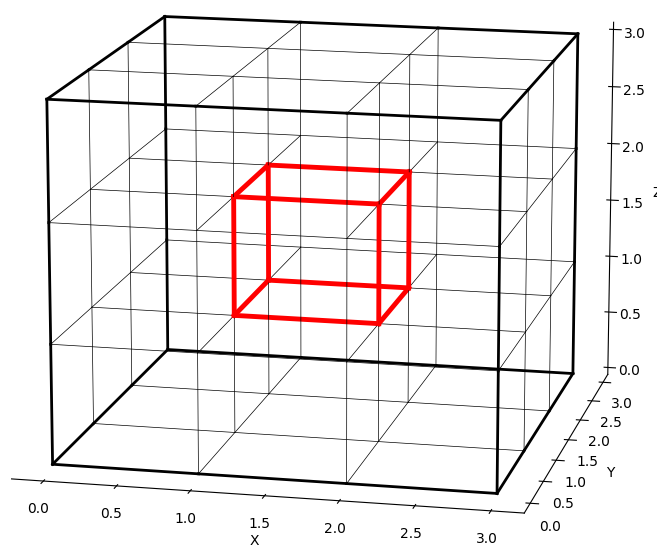
\includegraphics[width=0.7\linewidth]{images/3D_grid_example.png}
	\caption{Расчетная область}
	\label{fig:exampleOfArea}
\end{figure}

Тестирование будем проводить дифференциального уравнения (\ref{eq_4_2}):

\begin{equation} \label{eq_4_2}
	\text{rot} \left(\frac{1}{\mu} \text{rot} \overrightarrow{\textbf{A}}\right) + \gamma \overrightarrow{\textbf{A}} + \sigma \frac{\partial \overrightarrow{\textbf{A}}}{\partial t} = \overrightarrow{\textbf{F}}.
\end{equation}

В таблицах \ref{tab:test1} -- \ref{tab:test9} приведено тестирование на работоспособность программы. Для искомых $\overrightarrow{\textbf{A}}$ будем выводить значения функции в центрах рёбер сетки, отмеченных красным цветом на рисунке \ref{fig:exampleOfArea}.

\begin{table}
	\caption{Тестирование при $\overrightarrow{\textbf{A}} = (1.0, 1.0, 1.0)^{\text{T}}$, $\overrightarrow{\textbf{F}} = (1.0, 1.0, 1.0)^{\text{T}}$, $\mu = 1$, $\gamma = 1$, $\sigma = 0$}
	\centering
	\small
	\begin{tabularx}{1.0\textwidth}{| >{\raggedright\arraybackslash}X | >{\raggedright\arraybackslash}X | >{\raggedright\arraybackslash}X |>{\raggedright\arraybackslash}X |}
		\hline
		\centering{Ребро} & \centering{Значение} & \centering{Абсолютная погрешность} & \centering{Относительная погрешность} \tabularnewline \hline
		
		
		\centering{($x; 1.0; 1.0$)} & \centering{1.00000000E+000}& \centering{0.00000000E+000} & \centering{0.00000000E+000} \tabularnewline \hline
		
		\centering{($x; 2.0; 1.0$)} & \centering{1.00000000E+000}& \centering{0.00000000E+000} & \centering{0.00000000E+000} \tabularnewline \hline
		
		\centering{($x; 1.0; 2.0$)} & \centering{1.00000000E+000}& \centering{0.00000000E+000} & \centering{0.00000000E+000} \tabularnewline \hline
		
		\centering{($x; 2.0; 2.0$)} & \centering{1.00000000E+000}& \centering{0.00000000E+000} & \centering{0.00000000E+000} \tabularnewline \hline
		
		
		
		\centering{($1.0; y; 1.0$)} & \centering{1.00000000E+000}& \centering{0.00000000E+000} & \centering{0.00000000E+000} \tabularnewline \hline
		
		\centering{($2.0; y; 1.0$)} & \centering{1.00000000E+000}& \centering{0.00000000E+000} & \centering{0.00000000E+000} \tabularnewline \hline
		
		\centering{($1.0; y; 2.0$)} & \centering{1.00000000E+000}& \centering{0.00000000E+000} & \centering{0.00000000E+000} \tabularnewline \hline
		
		\centering{($2.0; y; 2.0$)} & \centering{1.00000000E+000}& \centering{0.00000000E+000} & \centering{0.00000000E+000} \tabularnewline \hline
		
		
		
		\centering{($1.0; 1.0; z$)} & \centering{1.00000000E+000}& \centering{0.00000000E+000} & \centering{0.00000000E+000} \tabularnewline \hline
		
		\centering{($2.0; 1.0; z$)} & \centering{1.00000000E+000}& \centering{0.00000000E+000} & \centering{0.00000000E+000} \tabularnewline \hline
		
		\centering{($1.0; 2.0; z$)} & \centering{1.00000000E+000}& \centering{0.00000000E+000} & \centering{0.00000000E+000} \tabularnewline \hline
		
		\centering{($2.0; 2.0; z$)} & \centering{1.00000000E+000}& \centering{0.00000000E+000} & \centering{0.00000000E+000} \tabularnewline \hline
		
		
	\end{tabularx}
	\label{tab:test1}
\end{table}

\begin{table}
	\caption{Тестирование при $\overrightarrow{\textbf{A}} = (y, z, x)^{\text{T}}$, $\overrightarrow{\textbf{F}} = (y, z, x)^{\text{T}}$, $\mu = 1$, $\gamma = 1$, $\sigma = 0$}
	\centering
	\small
	\begin{tabularx}{1.0\textwidth}{| >{\raggedright\arraybackslash}X | >{\raggedright\arraybackslash}X | >{\raggedright\arraybackslash}X |>{\raggedright\arraybackslash}X |}
		\hline
		\centering{Ребро} & \centering{Значение} & \centering{Абсолютная погрешность} & \centering{Относительная погрешность} \tabularnewline \hline
		
		\centering{($x; 1.0; 1.0$)} & \centering{1.00000000E+000}& \centering{0.00000000E+000} & \centering{0.00000000E+000} \tabularnewline \hline
		
		\centering{($x; 2.0; 1.0$)} & \centering{2.00000000E+000}& \centering{0.00000000E+000} & \centering{0.00000000E+000} \tabularnewline \hline
		
		\centering{($x; 1.0; 2.0$)} & \centering{1.00000000E+000}& \centering{0.00000000E+000} & \centering{0.00000000E+000} \tabularnewline \hline
		
		\centering{($x; 2.0; 2.0$)} & \centering{2.00000000E+000}& \centering{0.00000000E+000} & \centering{0.00000000E+000} \tabularnewline \hline
		
		
		
		\centering{($1.0; y; 1.0$)} & \centering{1.00000000E+000}& \centering{0.00000000E+000} & \centering{0.00000000E+000} \tabularnewline \hline
		
		\centering{($2.0; y; 1.0$)} & \centering{1.00000000E+000}& \centering{0.00000000E+000} & \centering{0.00000000E+000} \tabularnewline \hline
		
		\centering{($1.0; y; 2.0$)} & \centering{2.00000000E+000}& \centering{0.00000000E+000} & \centering{0.00000000E+000} \tabularnewline \hline
		
		\centering{($2.0; y; 2.0$)} & \centering{2.00000000E+000}& \centering{0.00000000E+000} & \centering{0.00000000E+000} \tabularnewline \hline
		
		
		
		\centering{($1.0; 1.0; z$)} & \centering{1.00000000E+000}& \centering{0.00000000E+000} & \centering{0.00000000E+000} \tabularnewline \hline
		
		\centering{($2.0; 1.0; z$)} & \centering{2.00000000E+000}& \centering{0.00000000E+000} & \centering{0.00000000E+000} \tabularnewline \hline
		
		\centering{($1.0; 2.0; z$)} & \centering{1.00000000E+000}& \centering{0.00000000E+000} & \centering{0.00000000E+000} \tabularnewline \hline
		
		\centering{($2.0; 2.0; z$)} & \centering{2.00000000E+000}& \centering{0.00000000E+000} & \centering{0.00000000E+000} \tabularnewline \hline
		
		
	\end{tabularx}
	\label{tab:test2}
\end{table}

\begin{table}
	\caption{Тестирование при $\overrightarrow{\textbf{A}} = (1 + y + x; 1 + x + z; 1 + x + y)^{\text{T}}$, $\overrightarrow{\textbf{F}} = (1 + y + x; 1 + x + z; 1 + x + y)^{\text{T}}$, $\mu = 1$, $\gamma = 1$, $\sigma = 0$}
	\centering
	\small
	\begin{tabularx}{1.0\textwidth}{| >{\raggedright\arraybackslash}X | >{\raggedright\arraybackslash}X | >{\raggedright\arraybackslash}X |>{\raggedright\arraybackslash}X |}
		\hline
		\centering{Ребро} & \centering{Значение} & \centering{Абсолютная погрешность} & \centering{Относительная погрешность} \tabularnewline \hline
		
		
		\centering{($x; 1.0; 1.0$)} & \centering{3.00000000E+000}& \centering{0.00000000E+000} & \centering{0.00000000E+000} \tabularnewline \hline
		
		\centering{($x; 2.0; 1.0$)} & \centering{4.00000000E+000}& \centering{0.00000000E+000} & \centering{0.00000000E+000} \tabularnewline \hline
		
		\centering{($x; 1.0; 2.0$)} & \centering{4.00000000E+000}& \centering{0.00000000E+000} & \centering{0.00000000E+000} \tabularnewline \hline
		
		\centering{($x; 2.0; 2.0$)} & \centering{5.00000000E+000}& \centering{0.00000000E+000} & \centering{0.00000000E+000} \tabularnewline \hline
		
		
		
		\centering{($1.0; y; 1.0$)} & \centering{3.00000000E+000}& \centering{0.00000000E+000} & \centering{0.00000000E+000} \tabularnewline \hline
		
		\centering{($2.0; y; 1.0$)} & \centering{4.00000000E+000}& \centering{0.00000000E+000} & \centering{0.00000000E+000} \tabularnewline \hline
		
		\centering{($1.0; y; 2.0$)} & \centering{4.00000000E+000}& \centering{0.00000000E+000} & \centering{0.00000000E+000} \tabularnewline \hline
		
		\centering{($2.0; y; 2.0$)} & \centering{5.00000000E+000}& \centering{0.00000000E+000} & \centering{0.00000000E+000} \tabularnewline \hline
		
		
		
		\centering{($1.0; 1.0; z$)} & \centering{3.00000000E+000}& \centering{0.00000000E+000} & \centering{0.00000000E+000} \tabularnewline \hline
		
		\centering{($2.0; 1.0; z$)} & \centering{4.00000000E+000}& \centering{0.00000000E+000} & \centering{0.00000000E+000} \tabularnewline \hline
		
		\centering{($1.0; 2.0; z$)} & \centering{4.00000000E+000}& \centering{0.00000000E+000} & \centering{0.00000000E+000} \tabularnewline \hline
		
		\centering{($2.0; 2.0; z$)} & \centering{5.00000000E+000}& \centering{0.00000000E+000} & \centering{0.00000000E+000} \tabularnewline \hline
		
	\end{tabularx}
	\label{tab:test3}
\end{table}

\begin{table}
	\caption{Тестирование при $\overrightarrow{\textbf{A}} = (y - z; x - z; x - y)^{\text{T}}$, $\overrightarrow{\textbf{F}} = (y - x; x - z; x - y)^{\text{T}}$, $\mu = 1$, $\gamma = 1$, $\sigma = 0$}
	\centering
	\small
	\begin{tabularx}{1.0\textwidth}{| >{\raggedright\arraybackslash}X | >{\raggedright\arraybackslash}X | >{\raggedright\arraybackslash}X |>{\raggedright\arraybackslash}X |}
		\hline
		\centering{Ребро} & \centering{Значение} & \centering{Абсолютная погрешность} & \centering{Относительная погрешность} \tabularnewline \hline
		
		
		\centering{($x; 1.0; 1.0$)} & \centering{2.35132600E-016}& \centering{2.35132600E-016} & \centering{0.00000000E+000} \tabularnewline \hline
		
		\centering{($x; 2.0; 1.0$)} & \centering{1.00000000E+000}& \centering{0.00000000E+000} & \centering{0.00000000E+000} \tabularnewline \hline
		
		\centering{($x; 1.0; 2.0$)} & \centering{-1.00000000E+000}& \centering{0.00000000E+000} & \centering{0.00000000E+000} \tabularnewline \hline
		
		\centering{($x; 2.0; 2.0$)} & \centering{-5.55111512E-016}& \centering{-5.55111512E-016} & \centering{0.00000000E+000} \tabularnewline \hline
		
		
		
		\centering{($1.0; y; 1.0$)} & \centering{-3.97378607E-016}& \centering{-3.97378607E-016} & \centering{0.00000000E+000} \tabularnewline \hline
		
		\centering{($2.0; y; 1.0$)} & \centering{1.00000000E+000}& \centering{0.00000000E+000} & \centering{0.00000000E+000} \tabularnewline \hline
		
		\centering{($1.0; y; 2.0$)} & \centering{-1.00000000E+000}& \centering{0.00000000E+000} & \centering{0.00000000E+000} \tabularnewline \hline
		
		\centering{($2.0; y; 2.0$)} & \centering{-1.94289029E-016}& \centering{-1.94289029E-016} & \centering{0.00000000E+000} \tabularnewline \hline
		
		
		
		\centering{($1.0; 1.0; z$)} & \centering{-2.74847895E-016}& \centering{-2.74847895E-016} & \centering{0.00000000E+000} \tabularnewline \hline
		
		\centering{($2.0; 1.0; z$)} & \centering{1.00000000E+000}& \centering{0.00000000E+000} & \centering{0.00000000E+000} \tabularnewline \hline
		
		\centering{($1.0; 2.0; z$)} & \centering{-1.00000000E+000}& \centering{0.00000000E+000} & \centering{0.00000000E+000} \tabularnewline \hline
		
		\centering{($2.0; 2.0; z$)} & \centering{4.27842044E-016}& \centering{4.27842044E-016} & \centering{0.00000000E+000} \tabularnewline \hline
		
		
	\end{tabularx}
	\label{tab:test4}
\end{table}

\begin{table}
	\caption{Тестирование при $\overrightarrow{\textbf{A}} = (y \cdot z; x \cdot z; x \cdot y)^{\text{T}}$, $\overrightarrow{\textbf{F}} = (y \cdot z; x \cdot z; x \cdot y)^{\text{T}}$, $\mu = 1$, $\gamma = 1$, $\sigma = 0$}
	\centering
	\small
	\begin{tabularx}{1.0\textwidth}{| >{\raggedright\arraybackslash}X | >{\raggedright\arraybackslash}X | >{\raggedright\arraybackslash}X |>{\raggedright\arraybackslash}X |}
		\hline
		\centering{Ребро} & \centering{Значение} & \centering{Абсолютная погрешность} & \centering{Относительная погрешность} \tabularnewline \hline
		
		
		\centering{($x; 1.0; 1.0$)} & \centering{1.00000000E+000}& \centering{0.00000000E+000} & \centering{0.00000000E+000} \tabularnewline \hline
		
		\centering{($x; 2.0; 1.0$)} & \centering{2.00000000E+000}& \centering{0.00000000E+000} & \centering{0.00000000E+000} \tabularnewline \hline
		
		\centering{($x; 1.0; 2.0$)} & \centering{2.00000000E+000}& \centering{0.00000000E+000} & \centering{0.00000000E+000} \tabularnewline \hline
		
		\centering{($x; 2.0; 2.0$)} & \centering{4.00000000E+000}& \centering{0.00000000E+000} & \centering{0.00000000E+000} \tabularnewline \hline
		
		
		
		\centering{($1.0; y; 1.0$)} & \centering{1.00000000E+000}& \centering{0.00000000E+000} & \centering{0.00000000E+000} \tabularnewline \hline
		
		\centering{($2.0; y; 1.0$)} & \centering{2.00000000E+000}& \centering{0.00000000E+000} & \centering{0.00000000E+000} \tabularnewline \hline
		
		\centering{($1.0; y; 2.0$)} & \centering{2.00000000E+000}& \centering{0.00000000E+000} & \centering{0.00000000E+000} \tabularnewline \hline
		
		\centering{($2.0; y; 2.0$)} & \centering{4.00000000E+000}& \centering{0.00000000E+000} & \centering{0.00000000E+000} \tabularnewline \hline
		
		\centering{($1.0; 1.0; z$)} & \centering{1.00000000E+000}& \centering{0.00000000E+000} & \centering{0.00000000E+000} \tabularnewline \hline
		
		\centering{($2.0; 1.0; z$)} & \centering{2.00000000E+000}& \centering{0.00000000E+000} & \centering{0.00000000E+000} \tabularnewline \hline
		
		\centering{($1.0; 2.0; z$)} & \centering{2.00000000E+000}& \centering{0.00000000E+000} & \centering{0.00000000E+000} \tabularnewline \hline
		
		\centering{($2.0; 2.0; z$)} & \centering{4.00000000E+000}& \centering{0.00000000E+000} & \centering{0.00000000E+000} \tabularnewline \hline
		
	\end{tabularx}
	\label{tab:test5}
\end{table}

\begin{table}
	\caption{Тестирование при $\overrightarrow{\textbf{A}} = (y^2; z^2; x^2)^{\text{T}}$, $\overrightarrow{\textbf{F}} = (y^2 - 2; z^2 - 2; x^2 - 2)^{\text{T}}$, $\mu = 1$, $\gamma = 1$, $\sigma = 0$}
	\centering
	\small
	\begin{tabularx}{1.0\textwidth}{| >{\raggedright\arraybackslash}X | >{\raggedright\arraybackslash}X | >{\raggedright\arraybackslash}X |>{\raggedright\arraybackslash}X |}
		\hline
		\centering{Ребро} & \centering{Значение} & \centering{Абсолютная погрешность} & \centering{Относительная погрешность} \tabularnewline \hline
		
		
		\centering{($x; 1.0; 1.0$)} & \centering{1.00000000E+000}& \centering{0.00000000E+000} & \centering{0.00000000E+000} \tabularnewline \hline
		
		\centering{($x; 2.0; 1.0$)} & \centering{4.00000000E+000}& \centering{0.00000000E+000} & \centering{0.00000000E+000} \tabularnewline \hline
		
		\centering{($x; 1.0; 2.0$)} & \centering{1.00000000E+000}& \centering{0.00000000E+000} & \centering{0.00000000E+000} \tabularnewline \hline
		
		\centering{($x; 2.0; 2.0$)} & \centering{4.00000000E+000}& \centering{0.00000000E+000} & \centering{0.00000000E+000} \tabularnewline \hline
		
		
		
		\centering{($1.0; y; 1.0$)} & \centering{1.00000000E+000}& \centering{0.00000000E+000} & \centering{0.00000000E+000} \tabularnewline \hline
		
		\centering{($2.0; y; 1.0$)} & \centering{1.00000000E+000}& \centering{0.00000000E+000} & \centering{0.00000000E+000} \tabularnewline \hline
		
		\centering{($1.0; y; 2.0$)} & \centering{4.00000000E+000}& \centering{0.00000000E+000} & \centering{0.00000000E+000} \tabularnewline \hline
		
		\centering{($2.0; y; 2.0$)} & \centering{4.00000000E+000}& \centering{0.00000000E+000} & \centering{0.00000000E+000} \tabularnewline \hline
		
		
		
		\centering{($1.0; 1.0; z$)} & \centering{1.00000000E+000}& \centering{0.00000000E+000} & \centering{0.00000000E+000} \tabularnewline \hline
		
		\centering{($2.0; 1.0; z$)} & \centering{4.00000000E+000}& \centering{0.00000000E+000} & \centering{0.00000000E+000} \tabularnewline \hline
		
		\centering{($1.0; 2.0; z$)} & \centering{1.00000000E+000}& \centering{0.00000000E+000} & \centering{0.00000000E+000} \tabularnewline \hline
		
		\centering{($2.0; 2.0; z$)} & \centering{4.00000000E+000}& \centering{0.00000000E+000} & \centering{0.00000000E+000} \tabularnewline \hline
	\end{tabularx}
	\label{tab:test6}
\end{table}

\begin{table}
	\caption{Тестирование при $\overrightarrow{\textbf{A}} = (y^2 + z^2; x^2 + z^2; x^2 + y^2)^{\text{T}}$, $\overrightarrow{\textbf{F}} = (y^2 + z^2 - 4; x^2 + z^2 - 4; x^2 + y^2 - 4)^{\text{T}}$, $\mu = 1$, $\gamma = 1$, $\sigma = 0$}
	\centering
	\small
	\begin{tabularx}{1.0\textwidth}{| >{\raggedright\arraybackslash}X | >{\raggedright\arraybackslash}X | >{\raggedright\arraybackslash}X |>{\raggedright\arraybackslash}X |}
		\hline
		\centering{Ребро} & \centering{Значение} & \centering{Абсолютная погрешность} & \centering{Относительная погрешность} \tabularnewline \hline
		
		
		\centering{($x; 1.0; 1.0$)} & \centering{2.00000000E+000}& \centering{0.00000000E+000} & \centering{0.00000000E+000} \tabularnewline \hline
		
		\centering{($x; 2.0; 1.0$)} & \centering{5.00000000E+000}& \centering{0.00000000E+000} & \centering{0.00000000E+000} \tabularnewline \hline
		
		\centering{($x; 1.0; 2.0$)} & \centering{5.00000000E+000}& \centering{0.00000000E+000} & \centering{0.00000000E+000} \tabularnewline \hline
		
		\centering{($x; 2.0; 2.0$)} & \centering{8.00000000E+000}& \centering{0.00000000E+000} & \centering{0.00000000E+000} \tabularnewline \hline
		
		
		
		\centering{($1.0; y; 1.0$)} & \centering{2.00000000E+000}& \centering{0.00000000E+000} & \centering{0.00000000E+000} \tabularnewline \hline
		
		\centering{($2.0; y; 1.0$)} & \centering{5.00000000E+000}& \centering{0.00000000E+000} & \centering{0.00000000E+000} \tabularnewline \hline
		
		\centering{($1.0; y; 2.0$)} & \centering{5.00000000E+000}& \centering{0.00000000E+000} & \centering{0.00000000E+000} \tabularnewline \hline
		
		\centering{($2.0; y; 2.0$)} & \centering{8.00000000E+000}& \centering{0.00000000E+000} & \centering{0.00000000E+000} \tabularnewline \hline
		
		
		
		\centering{($1.0; 1.0; z$)} & \centering{2.00000000E+000}& \centering{0.00000000E+000} & \centering{0.00000000E+000} \tabularnewline \hline
		
		\centering{($2.0; 1.0; z$)} & \centering{5.00000000E+000}& \centering{0.00000000E+000} & \centering{0.00000000E+000} \tabularnewline \hline
		
		\centering{($1.0; 2.0; z$)} & \centering{5.00000000E+000}& \centering{0.00000000E+000} & \centering{0.00000000E+000} \tabularnewline \hline
		
		\centering{($2.0; 2.0; z$)} & \centering{8.00000000E+000}& \centering{0.00000000E+000} & \centering{0.00000000E+000} \tabularnewline \hline
		
	\end{tabularx}
	\label{tab:test7}
\end{table}

\begin{table}
	\caption{Тестирование при $\overrightarrow{\textbf{A}} = (y^3; 0; 0)^{\text{T}}$, $\overrightarrow{\textbf{F}} = (y^3 - 6y; 0; 0)^{\text{T}}$, $\mu = 1$, $\gamma = 1$, $\sigma = 0$}
	\centering
	\small
	\begin{tabularx}{1.0\textwidth}{| >{\raggedright\arraybackslash}X | >{\raggedright\arraybackslash}X | >{\raggedright\arraybackslash}X |>{\raggedright\arraybackslash}X |}
		\hline
		\centering{Ребро} & \centering{Значение} & \centering{Абсолютная погрешность} & \centering{Относительная погрешность} \tabularnewline \hline
		
		
		\centering{($x; 1.0; 1.0$)} & \centering{1.00000000E+000}& \centering{0.00000000E+000} & \centering{0.00000000E+000} \tabularnewline \hline
		
		\centering{($x; 2.0; 1.0$)} & \centering{8.00000000E+000}& \centering{0.00000000E+000} & \centering{0.00000000E+000} \tabularnewline \hline
		
		\centering{($x; 1.0; 2.0$)} & \centering{1.00000000E+000}& \centering{0.00000000E+000} & \centering{0.00000000E+000} \tabularnewline \hline
		
		\centering{($x; 2.0; 2.0$)} & \centering{8.00000000E+000}& \centering{0.00000000E+000} & \centering{0.00000000E+000} \tabularnewline \hline
		
		
		
		\centering{($1.0; y; 1.0$)} & \centering{0.00000000E+000}& \centering{0.00000000E+000} & \centering{0.00000000E+000} \tabularnewline \hline
		
		\centering{($2.0; y; 1.0$)} & \centering{0.00000000E+000}& \centering{0.00000000E+000} & \centering{0.00000000E+000} \tabularnewline \hline
		
		\centering{($1.0; y; 2.0$)} & \centering{0.00000000E+000}& \centering{0.00000000E+000} & \centering{0.00000000E+000} \tabularnewline \hline
		
		\centering{($2.0; y; 2.0$)} & \centering{0.00000000E+000}& \centering{0.00000000E+000} & \centering{0.00000000E+000} \tabularnewline \hline
		
		
		
		\centering{($1.0; 1.0; z$)} & \centering{0.00000000E+000}& \centering{0.00000000E+000} & \centering{0.00000000E+000} \tabularnewline \hline
		
		\centering{($2.0; 1.0; z$)} & \centering{0.00000000E+000}& \centering{0.00000000E+000} & \centering{0.00000000E+000} \tabularnewline \hline
		
		\centering{($1.0; 2.0; z$)} & \centering{0.00000000E+000}& \centering{0.00000000E+000} & \centering{0.00000000E+000} \tabularnewline \hline
		
		\centering{($2.0; 2.0; z$)} & \centering{0.00000000E+000}& \centering{0.00000000E+000} & \centering{0.00000000E+000} \tabularnewline \hline
		
	\end{tabularx}
	\label{tab:test8}
\end{table}

\begin{table}
	\caption{Тестирование при $\overrightarrow{\textbf{A}} = (y^2 \cdot z^2; x^2 \cdot z^2; x^2 \cdot y^2)^{\text{T}}$, $\overrightarrow{\textbf{F}} = (y^2 \cdot z^2 - 2(y^2 + z^2); x^2 \cdot z^2 - 2(x^2 + z^2); x^2 \cdot y^2 - 2(x^2 + y^2))^{\text{T}}$, $\mu = 1$, $\gamma = 1$, $\sigma = 0$}
	\centering
	\small
	\begin{tabularx}{1.0\textwidth}{| >{\raggedright\arraybackslash}X | >{\raggedright\arraybackslash}X | >{\raggedright\arraybackslash}X |>{\raggedright\arraybackslash}X |}
		\hline
		\centering{Ребро} & \centering{Значение} & \centering{Абсолютная погрешность} & \centering{Относительная погрешность} \tabularnewline \hline
		
		
		\centering{($x; 1.0; 1.0$)} & \centering{1.00000000E+000}& \centering{0.00000000E+000} & \centering{0.00000000E+000} \tabularnewline \hline
		
		\centering{($x; 2.0; 1.0$)} & \centering{4.00000000E+000}& \centering{0.00000000E+000} & \centering{0.00000000E+000} \tabularnewline \hline
		
		\centering{($x; 1.0; 2.0$)} & \centering{4.00000000E+000}& \centering{0.00000000E+000} & \centering{0.00000000E+000} \tabularnewline \hline
		
		\centering{($x; 2.0; 2.0$)} & \centering{1.60000000E+001}& \centering{0.00000000E+000} & \centering{0.00000000E+000} \tabularnewline \hline
		
		
		
		\centering{($1.0; y; 1.0$)} & \centering{1.00000000E+000}& \centering{0.00000000E+000} & \centering{0.00000000E+000} \tabularnewline \hline
		
		\centering{($2.0; y; 1.0$)} & \centering{4.00000000E+000}& \centering{0.00000000E+000} & \centering{0.00000000E+000} \tabularnewline \hline
		
		\centering{($1.0; y; 2.0$)} & \centering{4.00000000E+000}& \centering{0.00000000E+000} & \centering{0.00000000E+000} \tabularnewline \hline
		
		\centering{($2.0; y; 2.0$)} & \centering{1.60000000E+001}& \centering{0.00000000E+000} & \centering{0.00000000E+000} \tabularnewline \hline
		
		
		
		\centering{($1.0; 1.0; z$)} & \centering{1.00000000E+000}& \centering{0.00000000E+000} & \centering{0.00000000E+000} \tabularnewline \hline
		
		\centering{($2.0; 1.0; z$)} & \centering{4.00000000E+000}& \centering{0.00000000E+000} & \centering{0.00000000E+000} \tabularnewline \hline
		
		\centering{($1.0; 2.0; z$)} & \centering{4.00000000E+000}& \centering{0.00000000E+000} & \centering{0.00000000E+000} \tabularnewline \hline
		
		\centering{($2.0; 2.0; z$)} & \centering{1.60000000E+001}& \centering{0.00000000E+000} & \centering{0.00000000E+000} \tabularnewline \hline
		
	\end{tabularx}
	\label{tab:test9}
\end{table}

Проведём тестирование на порядок аппроксимации. Для оценки будем брать значения вектор-функции в центрах параллелепипедов. Сетка по пространству для данных тестов изображена на рисунке \ref{fig:exampleOfArea_1}.

\begin{figure}
	\centering
	\vspace*{0.7cm}
	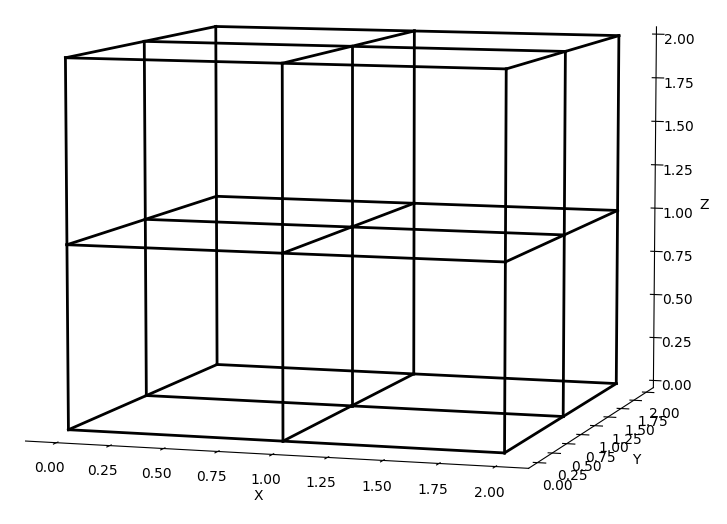
\includegraphics[width=0.5\linewidth]{images/3D_mesh_1.png}
	\caption{Расчетная область}
	\label{fig:exampleOfArea_1}
\end{figure}

В таблицах \ref{tab:test10} -- \ref{tab:test11} представлены результаты тестирования для постоянной и линейной вектор-функциях.

\begin{table}
	\caption{Тестирование при $\overrightarrow{\textbf{A}} = (1.0; 1.0; 1.0)^{\text{T}}$, $\overrightarrow{\textbf{F}} = (1.0; 1.0; 1.0)^{\text{T}}$, $\mu = 1$, $\gamma = 1$, $\sigma = 0$}
	\centering
	\small
	\begin{tabularx}{1.0\textwidth}{| >{\raggedright\arraybackslash}X | >{\raggedright\arraybackslash}X | >{\raggedright\arraybackslash}X |>{\raggedright\arraybackslash}X |}
		\hline
		\centering{Ребро} & \centering{Значение} & \centering{Абсолютная погрешность} & \centering{Относительная погрешность} \tabularnewline \hline
		
		
		\centering{($0.5; 0.5; 0.5$)} & \centering{1.00000000E+000 \\ 1.00000000E+000\\
			1.00000000E+000}& \centering{0.00000000E+000 \\ 0.00000000E+000 \\ 0.00000000E+000} & \centering{0.00000000E+000 \\ 0.00000000E+000 \\ 0.00000000E+000} \tabularnewline \hline
		
		\centering{($1.5; 0.5; 0.5$)} & \centering{1.00000000E+000 \\ 1.00000000E+000\\
			1.00000000E+000}& \centering{0.00000000E+000 \\ 0.00000000E+000 \\ 0.00000000E+000} & \centering{0.00000000E+000 \\ 0.00000000E+000 \\ 0.00000000E+000} \tabularnewline \hline
		
		\centering{($0.5; 1.5; 0.5$)} & \centering{1.00000000E+000 \\ 1.00000000E+000\\
			1.00000000E+000}& \centering{0.00000000E+000 \\ 0.00000000E+000 \\ 0.00000000E+000} & \centering{0.00000000E+000 \\ 0.00000000E+000 \\ 0.00000000E+000} \tabularnewline \hline
		
		\centering{($1.5; 1.5; 0.5$)} & \centering{1.00000000E+000 \\ 1.00000000E+000\\
			1.00000000E+000}& \centering{0.00000000E+000 \\ 0.00000000E+000 \\ 0.00000000E+000} & \centering{0.00000000E+000 \\ 0.00000000E+000 \\ 0.00000000E+000} \tabularnewline \hline
			
		\centering{($0.5; 0.5; 1.5$)} & \centering{1.00000000E+000 \\ 1.00000000E+000\\
			1.00000000E+000}& \centering{0.00000000E+000 \\ 0.00000000E+000 \\ 0.00000000E+000} & \centering{0.00000000E+000 \\ 0.00000000E+000 \\ 0.00000000E+000} \tabularnewline \hline
		
		\centering{($1.5; 0.5; 1.5$)} & \centering{1.00000000E+000 \\ 1.00000000E+000\\
			1.00000000E+000}& \centering{0.00000000E+000 \\ 0.00000000E+000 \\ 0.00000000E+000} & \centering{0.00000000E+000 \\ 0.00000000E+000 \\ 0.00000000E+000} \tabularnewline \hline
		
		\centering{($0.5; 1.5; 1.5$)} & \centering{1.00000000E+000 \\ 1.00000000E+000\\
			1.00000000E+000}& \centering{0.00000000E+000 \\ 0.00000000E+000 \\ 0.00000000E+000} & \centering{0.00000000E+000 \\ 0.00000000E+000 \\ 0.00000000E+000} \tabularnewline \hline
		
		\centering{($1.5; 1.5; 1.5$)} & \centering{1.00000000E+000 \\ 1.00000000E+000\\
			1.00000000E+000}& \centering{0.00000000E+000 \\ 0.00000000E+000 \\ 0.00000000E+000} & \centering{0.00000000E+000 \\ 0.00000000E+000 \\ 0.00000000E+000} \tabularnewline \hline
	
	\end{tabularx}
	\label{tab:test10}
\end{table}

\begin{table}
	\caption{Тестирование при $\overrightarrow{\textbf{A}} = (y; z; x)^{\text{T}}$, $\overrightarrow{\textbf{F}} = (y; z; x)^{\text{T}}$, $\mu = 1$, $\gamma = 1$, $\sigma = 0$}
	\centering
	\small
	\begin{tabularx}{1.0\textwidth}{| >{\raggedright\arraybackslash}X | >{\raggedright\arraybackslash}X | >{\raggedright\arraybackslash}X |>{\raggedright\arraybackslash}X |}
		\hline
		\centering{Ребро} & \centering{Значение} & \centering{Абсолютная погрешность} & \centering{Относительная погрешность} \tabularnewline \hline
		
		
		\centering{($0.5; 0.5; 0.5$)} & \centering{5.00000000E-001 \\ 5.00000000E-001 \\
			5.00000000E-001}& \centering{0.00000000E+000 \\ 0.00000000E+000 \\ 0.00000000E+000} & \centering{0.00000000E+000 \\ 0.00000000E+000 \\ 0.00000000E+000} \tabularnewline \hline
		
		\centering{($1.5; 0.5; 0.5$)} & \centering{5.00000000E-001 \\ 5.00000000E-001\\
			1.50000000E+000}& \centering{0.00000000E+000 \\ 0.00000000E+000 \\ 0.00000000E+000} & \centering{0.00000000E+000 \\ 0.00000000E+000 \\ 0.00000000E+000} \tabularnewline \hline
		
		\centering{($0.5; 1.5; 0.5$)} & \centering{1.50000000E+000 \\ 5.00000000E-001\\
			5.00000000E-001}& \centering{0.00000000E+000 \\ 0.00000000E+000 \\ 0.00000000E+000} & \centering{0.00000000E+000 \\ 0.00000000E+000 \\ 0.00000000E+000} \tabularnewline \hline
		
		\centering{($1.5; 1.5; 0.5$)} & \centering{1.50000000E+000 \\ 5.00000000E-001\\
			1.50000000E+000}& \centering{0.00000000E+000 \\ 0.00000000E+000 \\ 0.00000000E+000} & \centering{0.00000000E+000 \\ 0.00000000E+000 \\ 0.00000000E+000} \tabularnewline \hline
		
		\centering{($0.5; 0.5; 1.5$)} & \centering{5.00000000E-001 \\ 1.50000000E+000\\
			5.00000000E-001}& \centering{0.00000000E+000 \\ 0.00000000E+000 \\ 0.00000000E+000} & \centering{0.00000000E+000 \\ 0.00000000E+000 \\ 0.00000000E+000} \tabularnewline \hline
		
		\centering{($1.5; 0.5; 1.5$)} & \centering{5.00000000E-001 \\ 1.50000000E+000\\
			5.00000000E-001}& \centering{0.00000000E+000 \\ 0.00000000E+000 \\ 0.00000000E+000} & \centering{0.00000000E+000 \\ 0.00000000E+000 \\ 0.00000000E+000} \tabularnewline \hline
		
		\centering{($0.5; 1.5; 1.5$)} & \centering{1.50000000E+000 \\ 1.50000000E+000\\
			5.00000000E-001}& \centering{0.00000000E+000 \\ 0.00000000E+000 \\ 0.00000000E+000} & \centering{0.00000000E+000 \\ 0.00000000E+000 \\ 0.00000000E+000} \tabularnewline \hline
		
		\centering{($1.5; 1.5; 1.5$)} & \centering{1.50000000E+000 \\ 1.50000000E+000\\
			1.50000000E+000}& \centering{0.00000000E+000 \\ 0.00000000E+000 \\ 0.00000000E+000} & \centering{0.00000000E+000 \\ 0.00000000E+000 \\ 0.00000000E+000} \tabularnewline \hline
		
	\end{tabularx}
	\label{tab:test11}
\end{table}

Как и предполагали, при использовании билинейных вектор-функций точное решение находится вплоть до линейной вектор-функции без численной погрешности.

Проведём теперь тестирование на порядок сходимости на сетке изображённой на рисунке \ref{fig:exampleOfArea}. Для этого последовательно будем разбивать сетку в 2 раза сначала по оси $x$, потом по $y$ и затем по $z$. Результаты тестирования приведены в таблицах \ref{tab:test12} -- \ref{tab:test14}.

\begin{table}
	\caption{Тестирование при $\overrightarrow{\textbf{A}} = (0; 0; e^x)^{\text{T}}$, $\overrightarrow{\textbf{F}} = (0; 0; 0)^{\text{T}}$, $\mu = 1$, $\gamma = 1$, $\sigma = 0$}
	\centering
	\small
	\begin{tabularx}{1.0\textwidth}{| >{\raggedright\arraybackslash}X | >{\raggedright\arraybackslash}X | >{\raggedright\arraybackslash}X |>{\raggedright\arraybackslash}X |}
		\hline
		\centering{Шаг по оси $x$} & \centering{Средняя погрешность} & \centering{$\text{log}_2\left(\frac{\sigma_{i-1}}{\sigma_i}\right)$} \tabularnewline \hline		
		
		\centering{$h$} & \centering{4.1223218E-001} & \centering{-} \tabularnewline \hline
		
		\centering{${}^h/_2$} & \centering{6.9015889E-002} & \centering{2.57845668} \tabularnewline \hline
		
		\centering{${}^h/_4$} & \centering{1.4360912E-002} & \centering{2.26478117} \tabularnewline \hline
		
		\centering{${}^h/_8$} & \centering{3.28952607E-003} & \centering{2.1261957} \tabularnewline \hline
		
	\end{tabularx}
	\label{tab:test12}
\end{table}

\begin{table}
	\caption{Тестирование при $\overrightarrow{\textbf{A}} = (e^y; 0; 0)^{\text{T}}$, $\overrightarrow{\textbf{F}} = (0; 0; 0)^{\text{T}}$, $\mu = 1$, $\gamma = 1$, $\sigma = 0$}
	\centering
	\small
	\begin{tabularx}{1.0\textwidth}{| >{\raggedright\arraybackslash}X | >{\raggedright\arraybackslash}X | >{\raggedright\arraybackslash}X |>{\raggedright\arraybackslash}X |}
		\hline
		\centering{Шаг по оси $y$} & \centering{Средняя погрешность} & \centering{$\text{log}_2\left(\frac{\sigma_{i-1}}{\sigma_i}\right)$} \tabularnewline \hline		
		
		\centering{$h$} & \centering{4.1223218E-001} & \centering{-} \tabularnewline \hline

		\centering{${}^h/_2$} & \centering{6.9015889E-002} & \centering{2.57845668} \tabularnewline \hline

		\centering{${}^h/_4$} & \centering{1.4360912E-002} & \centering{2.26478117} \tabularnewline \hline

		\centering{${}^h/_8$} & \centering{3.28952607E-003} & \centering{2.1261957} \tabularnewline \hline
		
	\end{tabularx}
	\label{tab:test13}
\end{table}

\begin{table}
	\caption{Тестирование при $\overrightarrow{\textbf{A}} = (0; e^z; 0)^{\text{T}}$, $\overrightarrow{\textbf{F}} = (0; 0; 0)^{\text{T}}$, $\mu = 1$, $\gamma = 1$, $\sigma = 0$}
	\centering
	\small
	\begin{tabularx}{1.0\textwidth}{| >{\raggedright\arraybackslash}X | >{\raggedright\arraybackslash}X | >{\raggedright\arraybackslash}X |>{\raggedright\arraybackslash}X |}
		\hline
		\centering{Шаг по оси $z$} & \centering{Средняя погрешность} & \centering{$\text{log}_2\left(\frac{\sigma_{i-1}}{\sigma_i}\right)$} \tabularnewline \hline		
		
		\centering{$h$} & \centering{4.1223218E-001} & \centering{-} \tabularnewline \hline
		
		\centering{${}^h/_2$} & \centering{6.9015889E-002} & \centering{2.57845668} \tabularnewline \hline
		
		\centering{${}^h/_4$} & \centering{1.4360912E-002} & \centering{2.26478117} \tabularnewline \hline
		
		\centering{${}^h/_8$} & \centering{3.28952607E-003} & \centering{2.1261957} \tabularnewline \hline
		
	\end{tabularx}
	\label{tab:test14}
\end{table}

Во всех трёх случая порядок сходимости стремится к 2. Исходя из полученных данных, можно сказать, что программа верно находит численное решение эллиптической задачи.

\section{Проверка полученных результатов}

Проверку полученных результатов решения СЛАУ будем из закона индукции Фарадея (\ref{eq_1_2}) и теоремы о циркуляции магнитного поля (\ref{eq_1_1}). Учитывая (\ref{eq_2_27}) -- (\ref{eq_2_29}), получим выражение для $\overrightarrow{\textbf{B}}$, которое будем использовать для проверки:

\begin{equation} \label{eq_3_1}
	\overrightarrow{\textbf{B}} = \text{rot} \overrightarrow{\textbf{A}} = 
	\begin{vmatrix}
		\textbf{i} & \textbf{j} & \textbf{k}\\
		\frac{\partial}{\partial x} & \frac{\partial}{\partial y} & \frac{\partial}{\partial z}\\
		A_x & A_y & 0
	\end{vmatrix}
	= -\frac{\partial A_y}{\partial z} \textbf{i} + \frac{\partial A_x}{\partial z} \textbf{j} + \left(\frac{\partial A_y}{\partial x} - \frac{\partial A_x}{\partial y}\right) \textbf{k}.
\end{equation}

Исходя из теории конечно-разностных схем \cite{10}, численно определим значения для частных первых производных в выражении (\ref{eq_3_1}):

\begin{equation} \label{eq_3_2}
	\frac{\partial A_{x_i}}{\partial x_k} + o\left(h_{x_k}^3\right) = \frac{A_{x_i}^{j+1} - A_{x_i}^{j-1}}{2h_{x_k}},
\end{equation}
где $x_k$ -- переменная по которой проводится дифференцирование, $x_i$ -- соответствующая компонента вектора-потенциала $\overrightarrow{\textbf{A}}$, $A_{x_i}^{j+1} = A_{x_i}\left(x_{0i} + h_{x_k}\right)$, $A_{x_i}^{j-1} = A_{x_{i}}\left(x_{0i} - h_{x_k}\right)$, $h_{x_k}$ -- шаг от точки, в которой необходимо найти значение производной, равный $10^{-10}$.

%\textbf{Здесь будет программная реализация $\downarrow$}


\chapter{Исследования}

\section{Исследование первичного поля}

Пусть источник индукционного поля лежит на расстоянии $R = 500$ м от оси симметрии и имееет силу тока, равную $J_{\varphi} = 1.0$ А. Также условимся, что источник работал достаточно долго, чтобы создать стабильное электромагнитное поле. Сетка по времени равномерная: $t=[1.0; 1.05]$ на 200 временных слоёв. После истечения первой секунды мы отключим наш источник, т.е. $J_{\varphi} = 0.0$ A при $t > 1.0$. На рисунках \ref{fig:A_phi_0} -- \ref{fig:E_phi_2} представлено распространение этого поля в среде в начальный, промежуточных и последний момент времени.

\begin{figure}
	\centering
	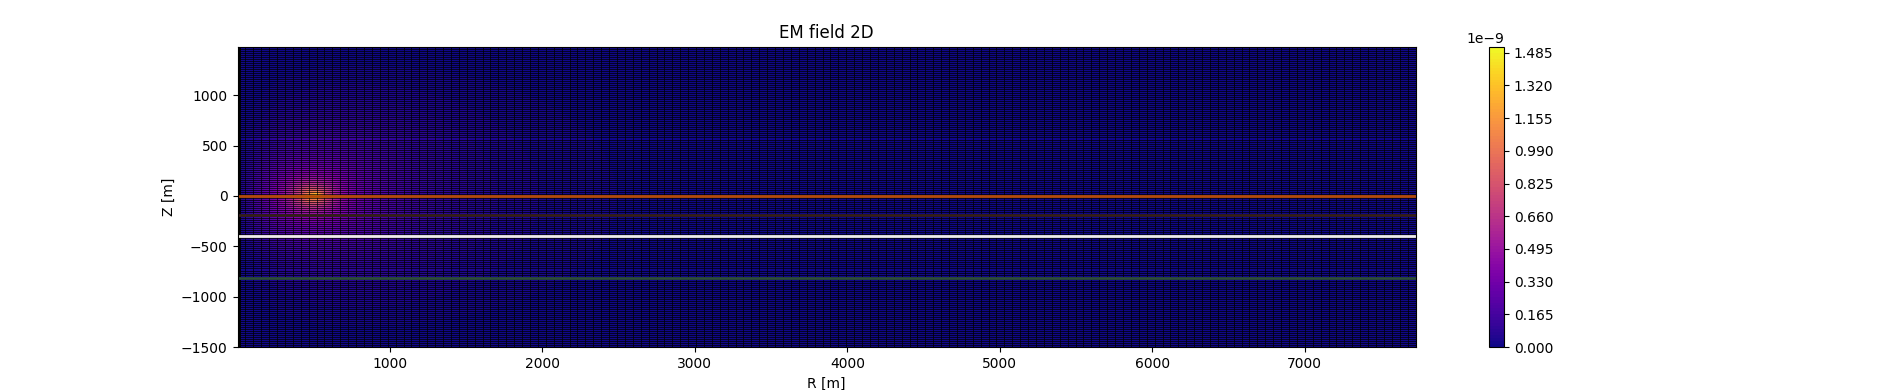
\includegraphics[width=1.0\linewidth]{images/Answer_A_time_layer_1.png}
	\caption{Решение $A_{\varphi}$ при $t = 1.0с$}
	\label{fig:A_phi_0}
\end{figure}

\begin{figure}
	\centering
	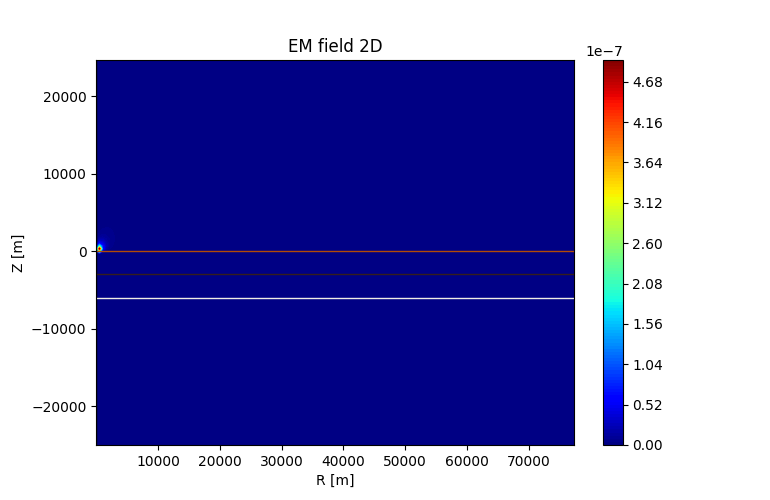
\includegraphics[width=1.0\linewidth]{images/Answer_E_time_layer_1.png}
	\caption{Решение $E_{\varphi}$ при $t = 1.0с$}
	\label{fig:E_phi_0}
\end{figure}

\begin{figure}
	\centering
	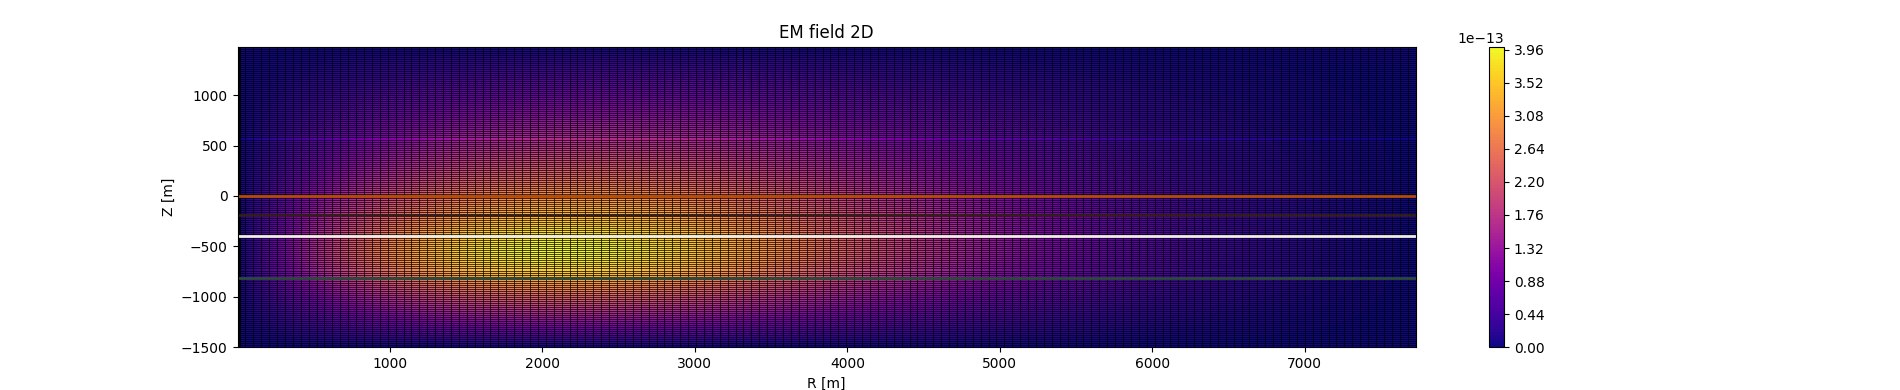
\includegraphics[width=1.0\linewidth]{images/Answer_A_time_layer_1.0250000000000083.png}
	\caption{Решение $A_{\varphi}$ при $t = 1.025с$}
	\label{fig:A_phi_1}
\end{figure}

\begin{figure}
	\centering
	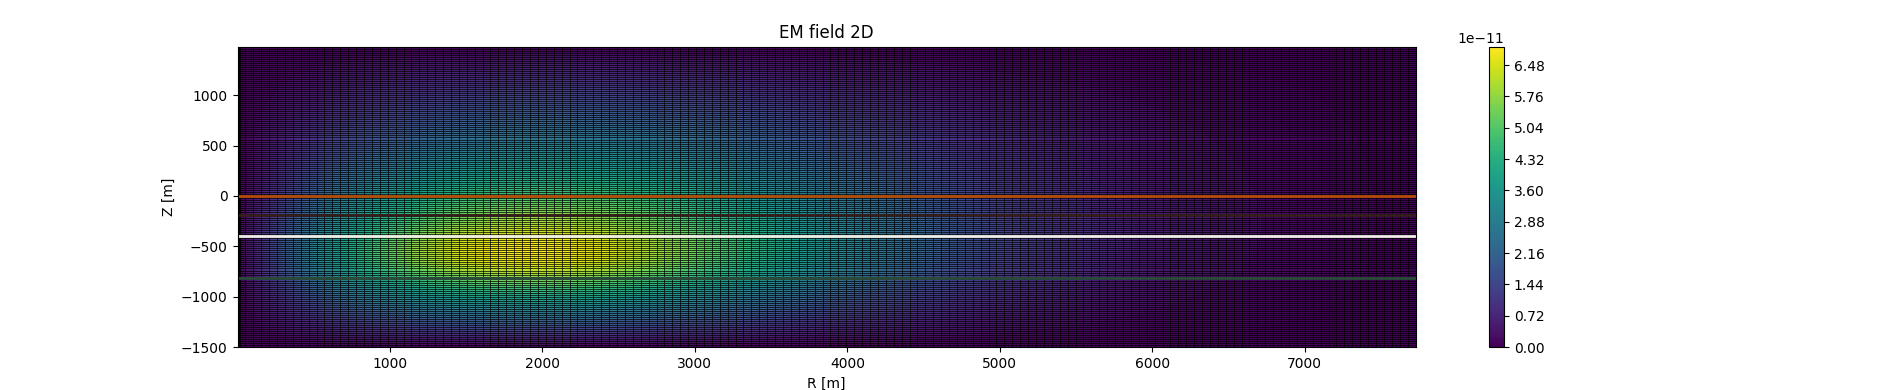
\includegraphics[width=1.0\linewidth]{images/Answer_E_time_layer_1.0250000000000083.png}
	\caption{Решение $E_{\varphi}$ при $t = 1.025с$}
	\label{fig:E_phi_1}
\end{figure} 

\begin{figure}
	\centering
	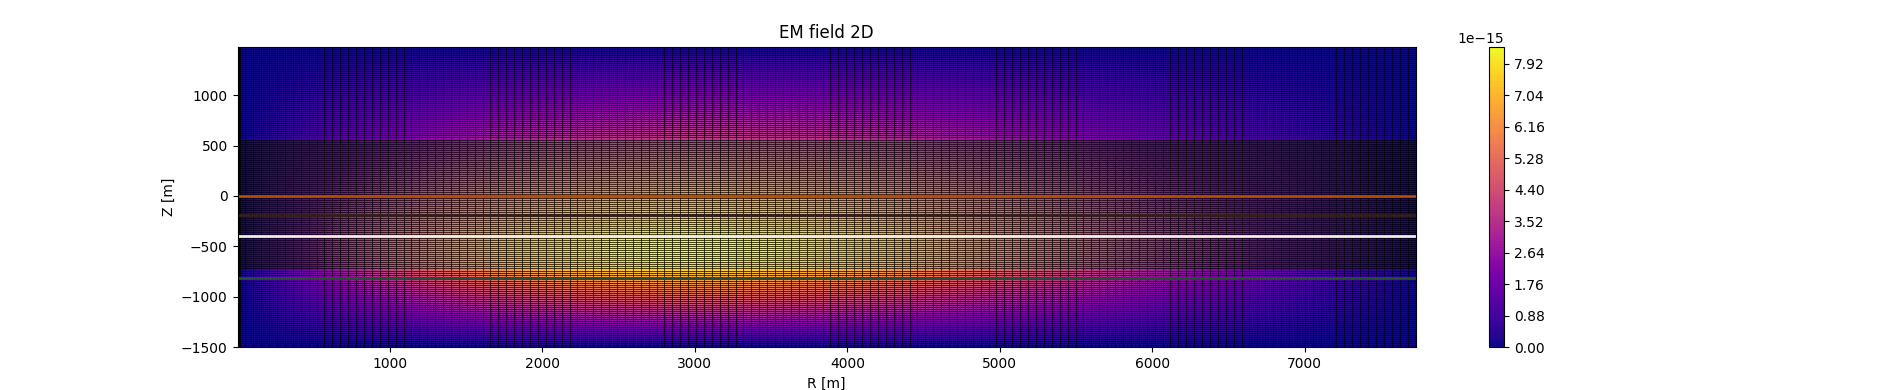
\includegraphics[width=1.0\linewidth]{images/Answer_A_time_layer_1.05.png}
	\caption{Решение $A_{\varphi}$ при $t = 1.05с$}
	\label{fig:A_phi_2}
\end{figure}

\begin{figure}
	\centering
	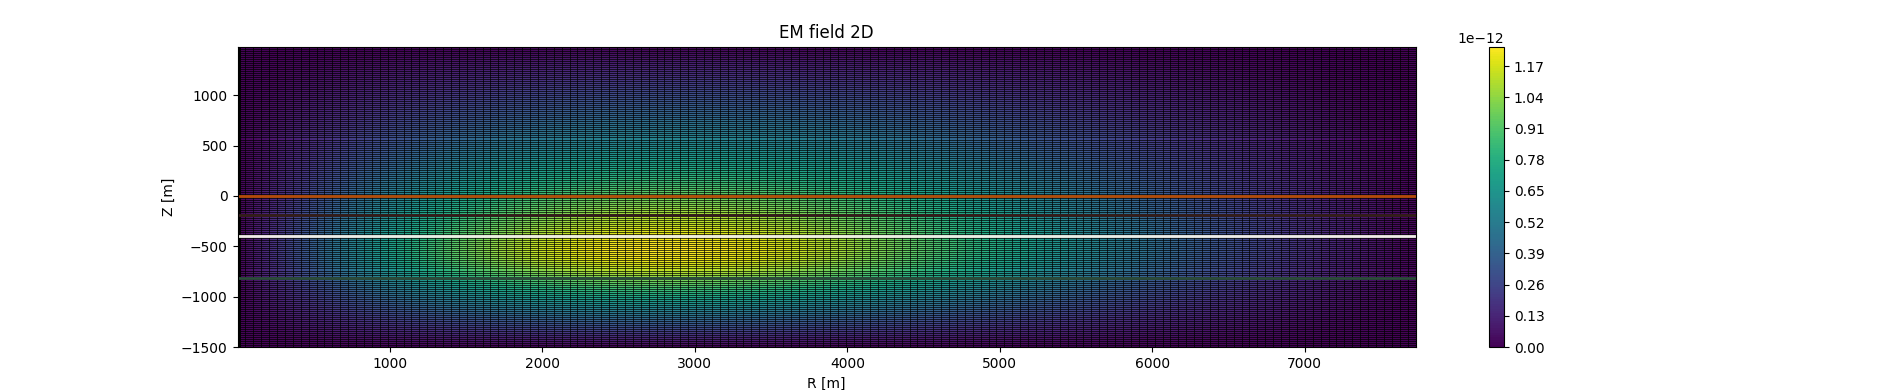
\includegraphics[width=1.0\linewidth]{images/Answer_E_time_layer_1.05.png}
	\caption{Решение $A_{\varphi}$ при $t = 1.05с$}
	\label{fig:E_phi_2}
\end{figure} 

Расположим на расчётной области приёмники в каждой горизонтально-слоистой среде и проведем замеры значений вектор-потенциала и электрического поля в точках $(2500; 0; -100)$, $(2500; 0; -200)$, $(10; 0; -700)$, $(1000; 0; -1250)$. Отобразим на графиках \ref{fig:NatA} -- \ref{fig:LogE} полученные значения.

\begin{figure}
	\centering
	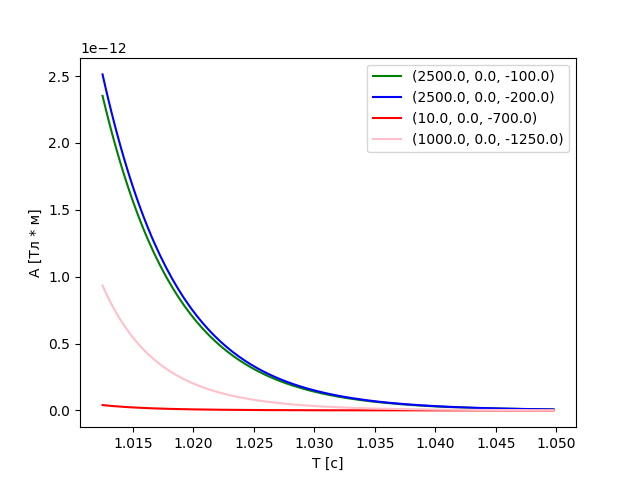
\includegraphics[width=0.8\linewidth]{images/Normal_A.png}
	\caption{Зависимость значения $A_{\varphi}$ от времени в разных приёмниках}
	\label{fig:NatA}
\end{figure}

\begin{figure}
	\centering
	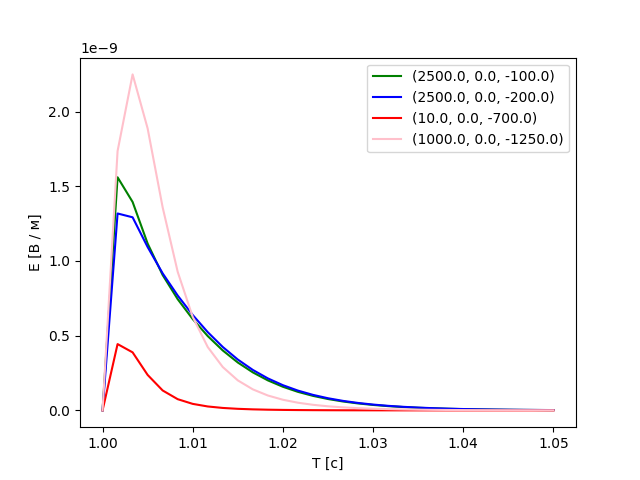
\includegraphics[width=0.8\linewidth]{images/Normal_E.png}
	\caption{Зависимость значения $E_{\varphi}$ от времени в разных приёмниках}
	\label{fig:NatE}
\end{figure}


\begin{figure}
	\centering
	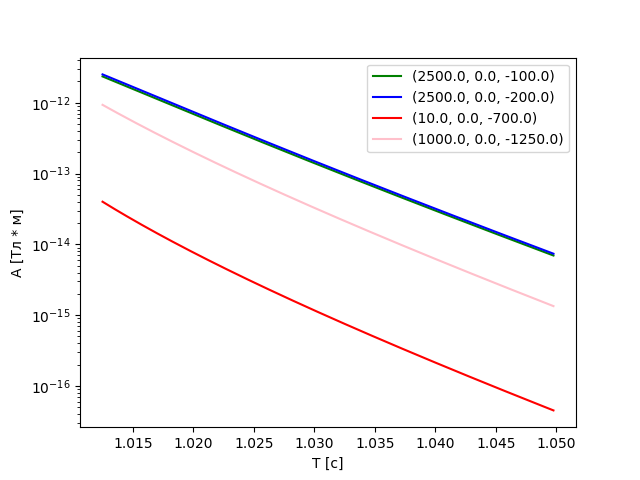
\includegraphics[width=0.8\linewidth]{images/Log_A.png}
	\caption{Зависимость значения $A_{\varphi}$ от времени в разных приёмниках (логарифмическая шкала по оси абсцисс)}
	\label{fig:LogA}
\end{figure}

\begin{figure}
	\centering
	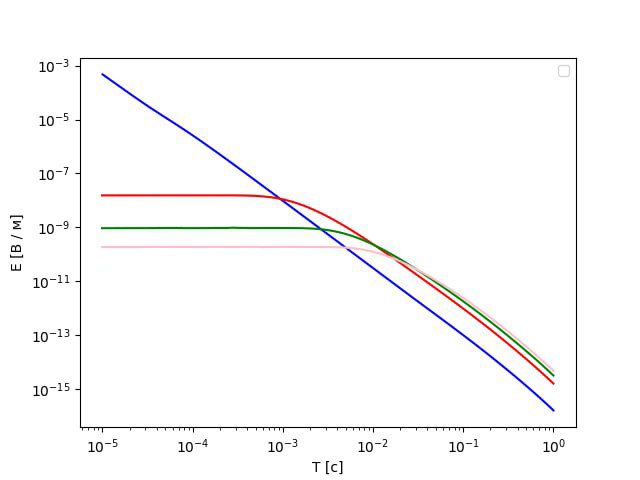
\includegraphics[width=0.8\linewidth]{images/Log_E.png}
	\caption{Зависимость значения $E_{\varphi}$ от времени в разных приёмниках (логарифмическая шкала по оси абсцисс)}
	\label{fig:LogE}
\end{figure} 

Как видим, значения вектор-потенциала и электрической напряжённости поля не имеют каких-либо резких колебаний. Из этого можно заключить, что, как и предполагалось, никаких аномальных зон в исследуемой области нет. 

\section{Исследование при разделении нормального и добавочного поля}

Добавим в нашу область аномальный объект со следующими границами: $[-5500; 5500]_x \times [2205; 2355]_y \times [-180; -80]_z$ и значением $\sigma = 4$. Будем искать решение из уравнения на добавочное поле (\ref{eq_1_6}). Получим решения изображенные на рисунках \ref{fig:A_plus_t0} -- \ref{fig:E_plus_t2}.

\begin{figure}
	\centering
	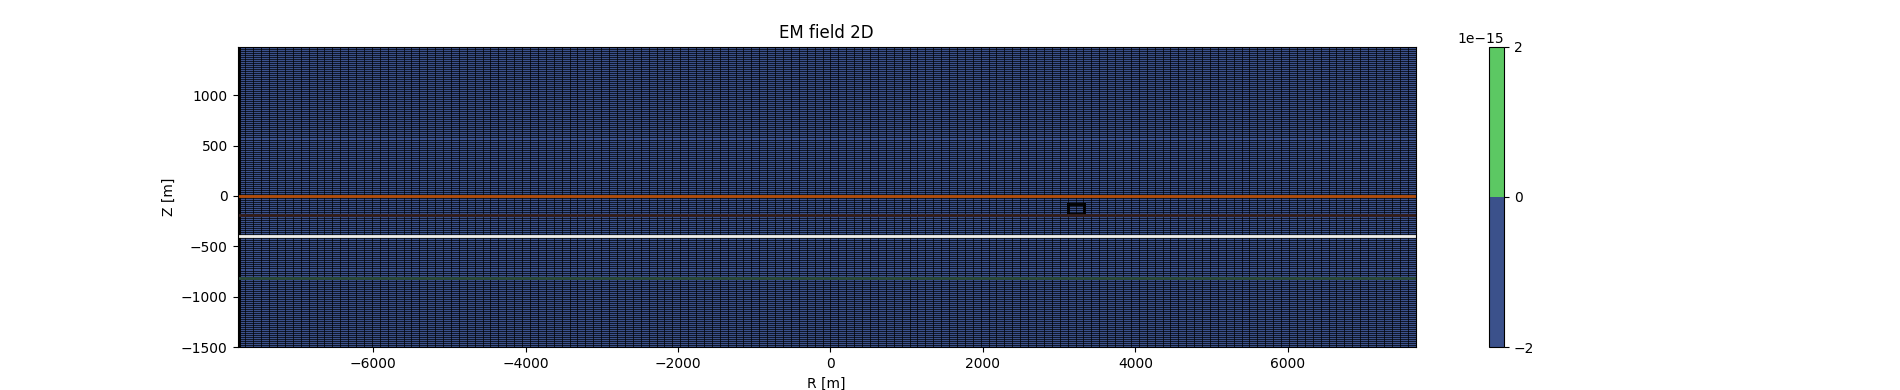
\includegraphics[width=1.0\linewidth]{images/Answer_A_plus_time_layer_1.png}
	\caption{Решение $\overrightarrow{\textbf{A}}^+$ при $t = 1.0с$}
	\label{fig:A_plus_t0}
\end{figure} 


\begin{figure}
	\centering
	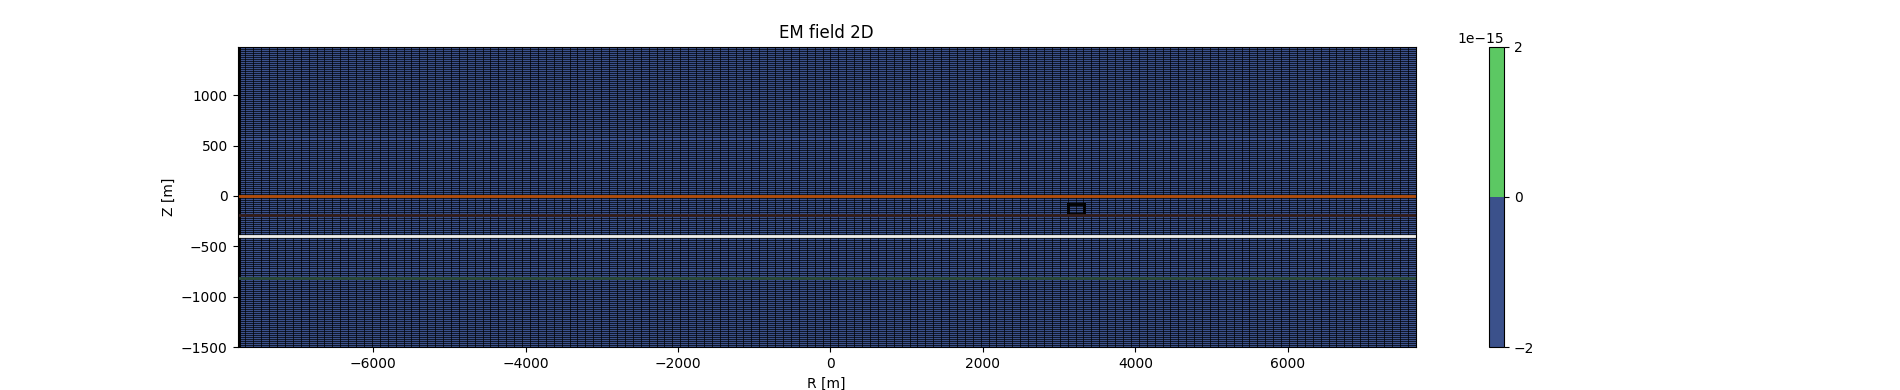
\includegraphics[width=1.0\linewidth]{images/Answer_E_plus_time_layer_1.png}
	\caption{Решение $\overrightarrow{\textbf{E}}^+$ при $t = 1.0с$}
	\label{fig:E_plus_t0}
\end{figure} 


\begin{figure}
	\centering
	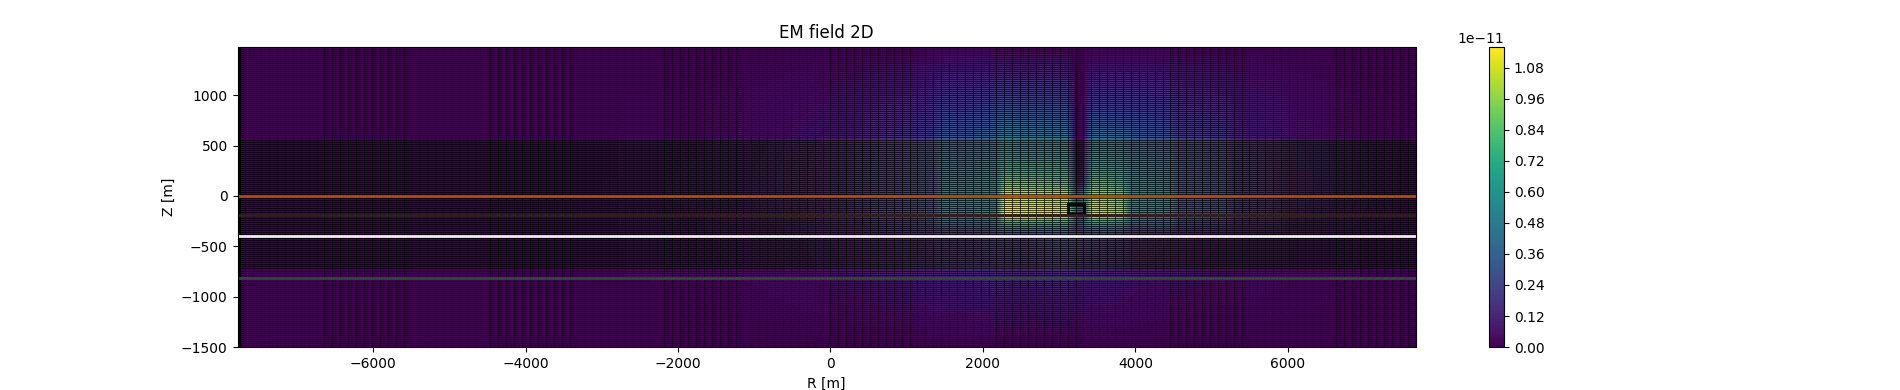
\includegraphics[width=1.0\linewidth]{images/Answer_A_plus_time_layer_1.0250000000000006.png}
	\caption{Решение $\overrightarrow{\textbf{A}}^+$ при $t = 1.025с$}
	\label{fig:A_plus_t1}
\end{figure} 


\begin{figure}
	\centering
	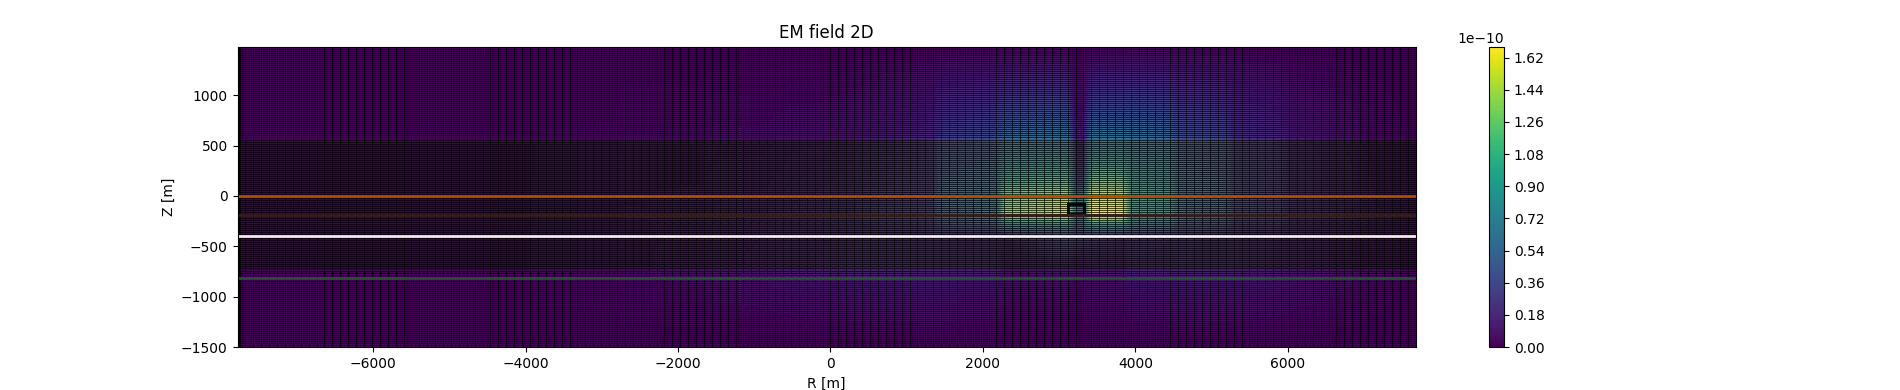
\includegraphics[width=1.0\linewidth]{images/Answer_E_plus_time_layer_1.0250000000000006.png}
	\caption{Решение $\overrightarrow{\textbf{E}}^+$ при $t = 1.025с$}
	\label{fig:E_plus_t1}
\end{figure} 

\begin{figure}
	\centering
	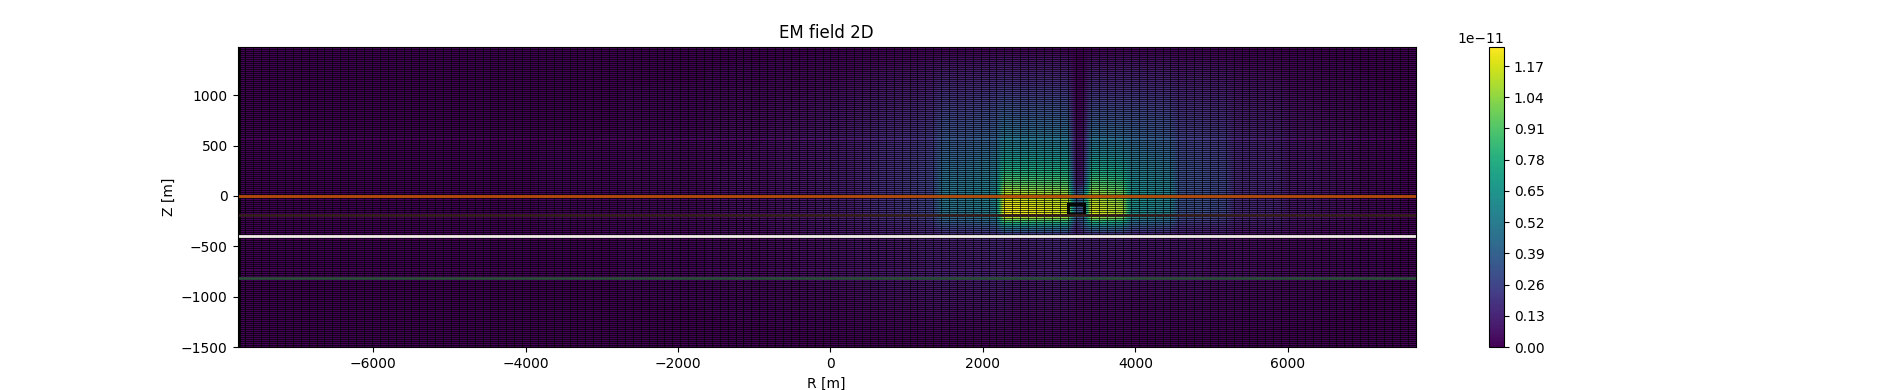
\includegraphics[width=1.0\linewidth]{images/Answer_A_plus_time_layer_1.05.png}
	\caption{Решение $\overrightarrow{\textbf{A}}^+$ при $t = 1.05с$}
	\label{fig:A_plus_t2}
\end{figure} 


\begin{figure}
	\centering
	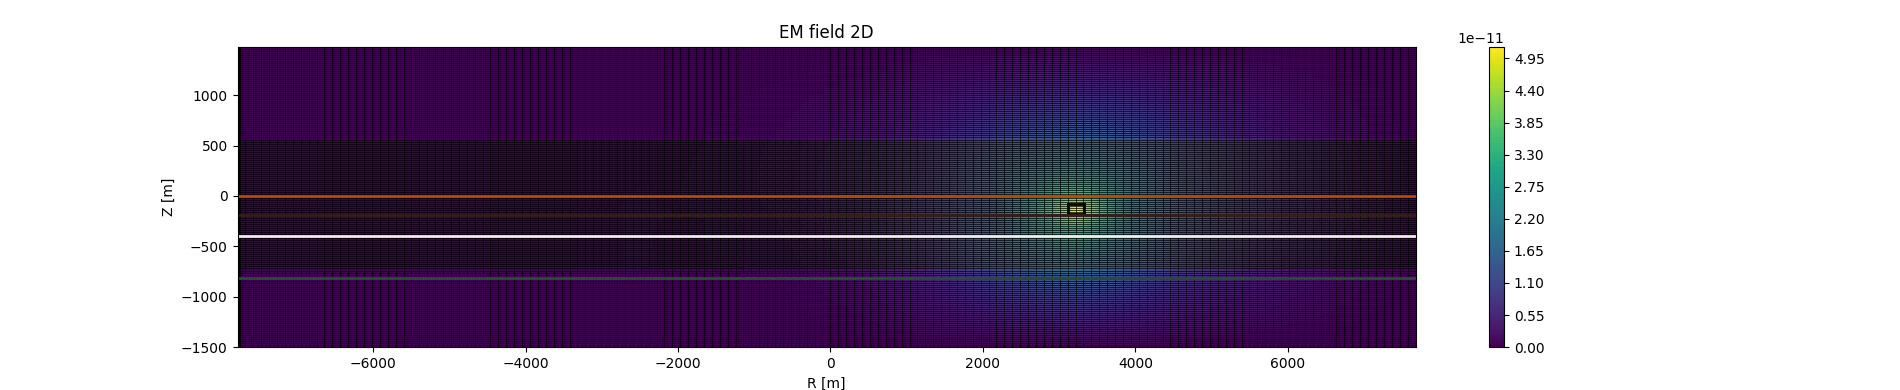
\includegraphics[width=1.0\linewidth]{images/Answer_E_plus_time_layer_1.05.png}
	\caption{Решение $\overrightarrow{\textbf{E}}^+$ при $t = 1.05с$}
	\label{fig:E_plus_t2}
\end{figure} 

Рассмотрим для $t = 1.0, t = 1.025, t = 1.05$ значения $\overrightarrow{\textbf{A}}^+$ и $\overrightarrow{\textbf{E}}^+$ на линии, перпендикулярно проходящей к аномальному объекту по оси $y$ при $x = 0.0, z = -130.0$. Получим следующее:

\begin{figure}
	\centering
	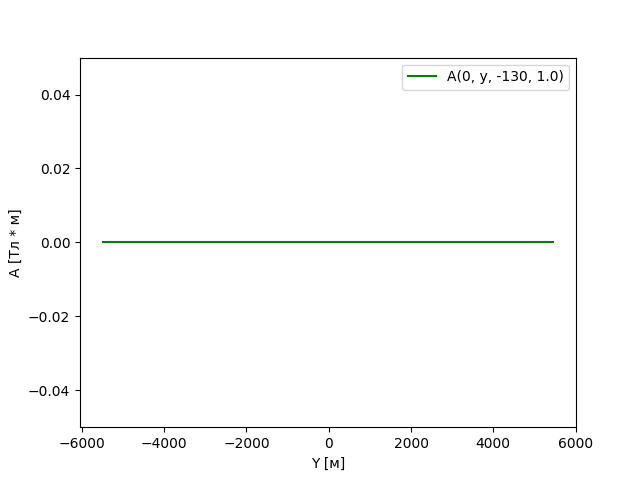
\includegraphics[width=0.5\linewidth]{images/Normal_A(y)_1.png}
	\caption{Решение $\overrightarrow{\textbf{A}}^+$ на линии $(0.0, y, -130.0)$ при $t = 1.0с$}
	\label{fig:A_line_t0}
\end{figure} 

\begin{figure}
	\centering
	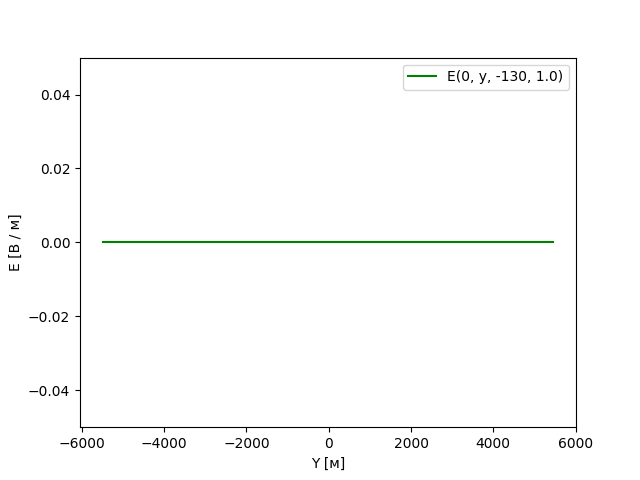
\includegraphics[width=0.5\linewidth]{images/Normal_E(y)_1.png}
	\caption{Решение $\overrightarrow{\textbf{E}}^+$ на линии $(0.0, y, -130.0)$ при $t = 1.0с$}
	\label{fig:E_line_t0}
\end{figure} 

\begin{figure}
	\centering
	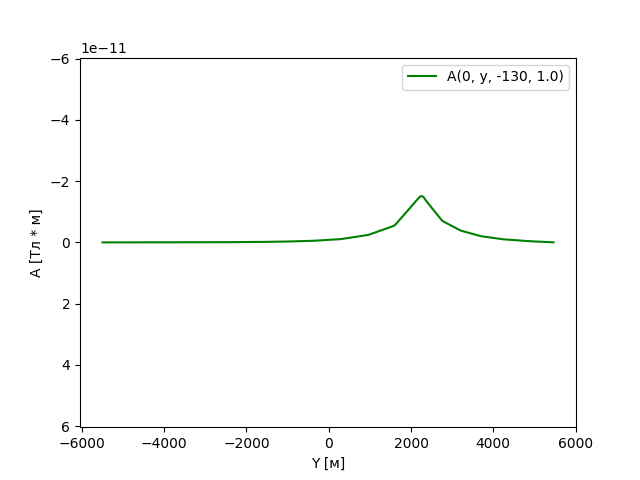
\includegraphics[width=0.5\linewidth]{images/Normal_A(y)_2.png}
	\caption{Решение $\overrightarrow{\textbf{A}}^+$ на линии $(0.0, y, -130.0)$ при $t = 1.025с$}
	\label{fig:A_line_t1}
\end{figure} 

\begin{figure}
	\centering
	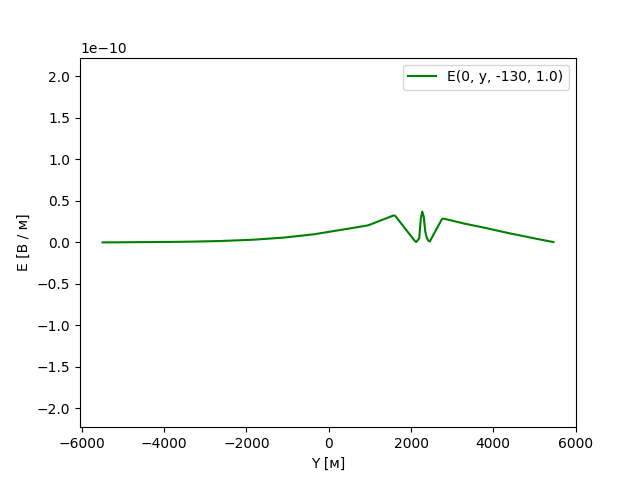
\includegraphics[width=0.5\linewidth]{images/Normal_E(y)_2.png}
	\caption{Решение $\overrightarrow{\textbf{E}}^+$ на линии $(0.0, y, -130.0)$  при $t = 1.025с$}
	\label{fig:E_line_t1}
\end{figure} 

\begin{figure}
	\centering
	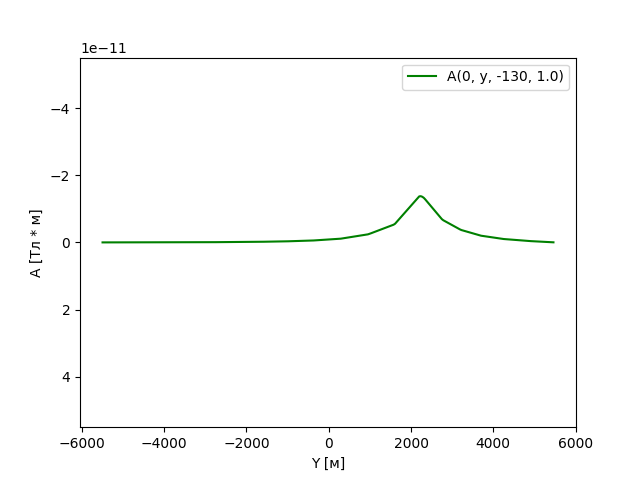
\includegraphics[width=0.5\linewidth]{images/Normal_A(y)_3.png}
	\caption{Решение $\overrightarrow{\textbf{A}}^+$ на линии $(0.0, y, -130.0)$  при $t = 1.05с$}
	\label{fig:A_line_t2}
\end{figure} 

\begin{figure}
	\centering
	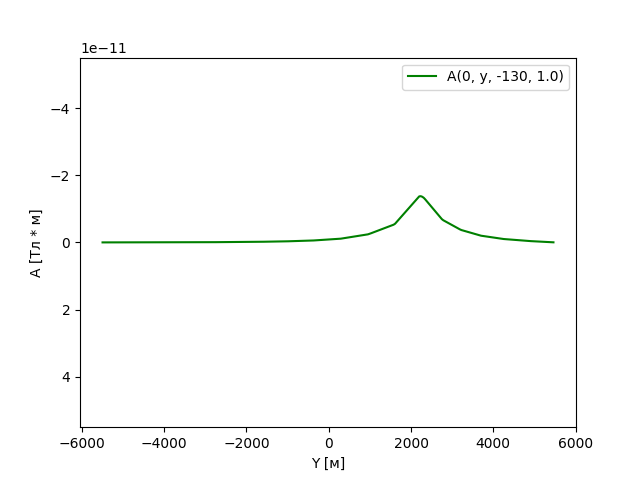
\includegraphics[width=0.5\linewidth]{images/Normal_A(y)_3.png}
	\caption{Решение $\overrightarrow{\textbf{A}}^+$ на линии $(0.0, y, -130.0)$  при $t = 1.05с$}
	\label{fig:E_line_t2}
\end{figure} 


Суммируем полученный результат с нормальным полем и получим состояние поля в разные моменты времени, изображённые на рисунках \ref{fig:A_Istage_t0} -- \ref{fig:E_Istage_t2}.

\begin{figure}
	\centering
	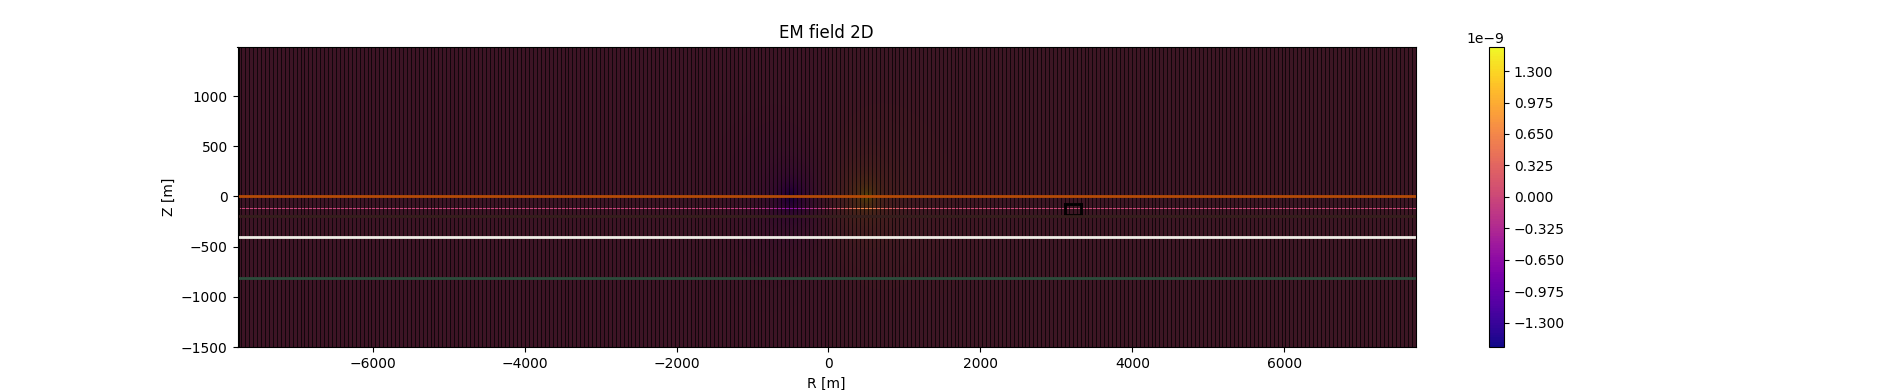
\includegraphics[width=1.0\linewidth]{images/Answer_A_Istage_time_layer_1.png}
	\caption{Решение суммарного поля $\overrightarrow{\textbf{A}}$ при $t = 1.0с$}
	\label{fig:A_Istage_t0}
\end{figure} 


\begin{figure}
	\centering
	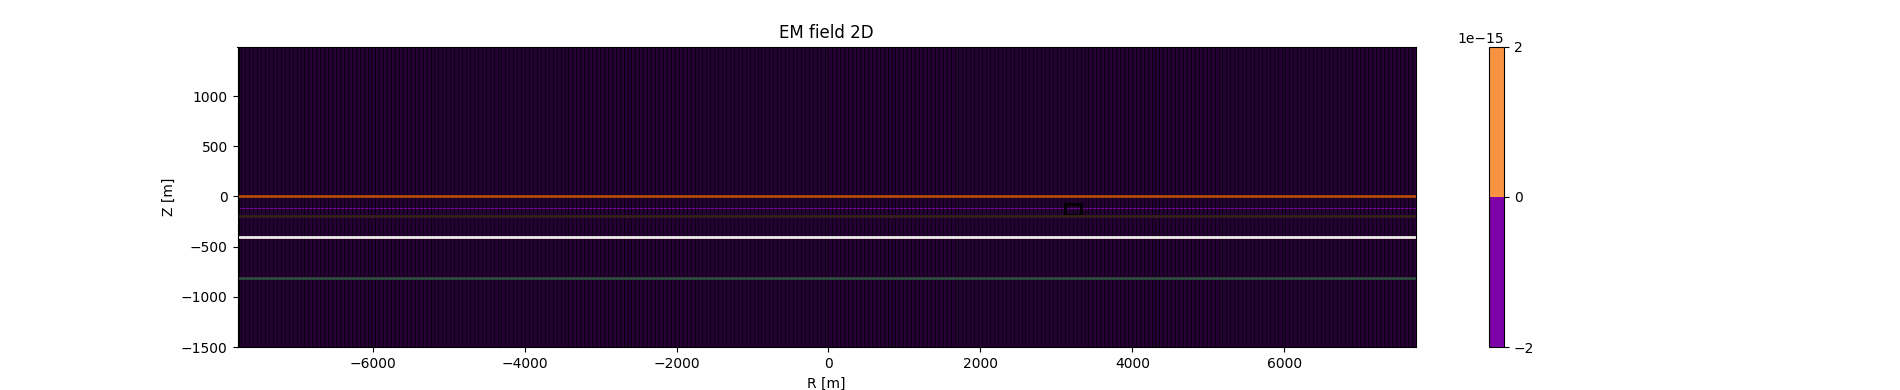
\includegraphics[width=1.0\linewidth]{images/Answer_E_Istage_time_layer_1.png}
	\caption{Решение суммарного поля $\overrightarrow{\textbf{E}}$ при $t = 1.0с$}
	\label{fig:E_Istage_t0}
\end{figure} 


\begin{figure}
	\centering
	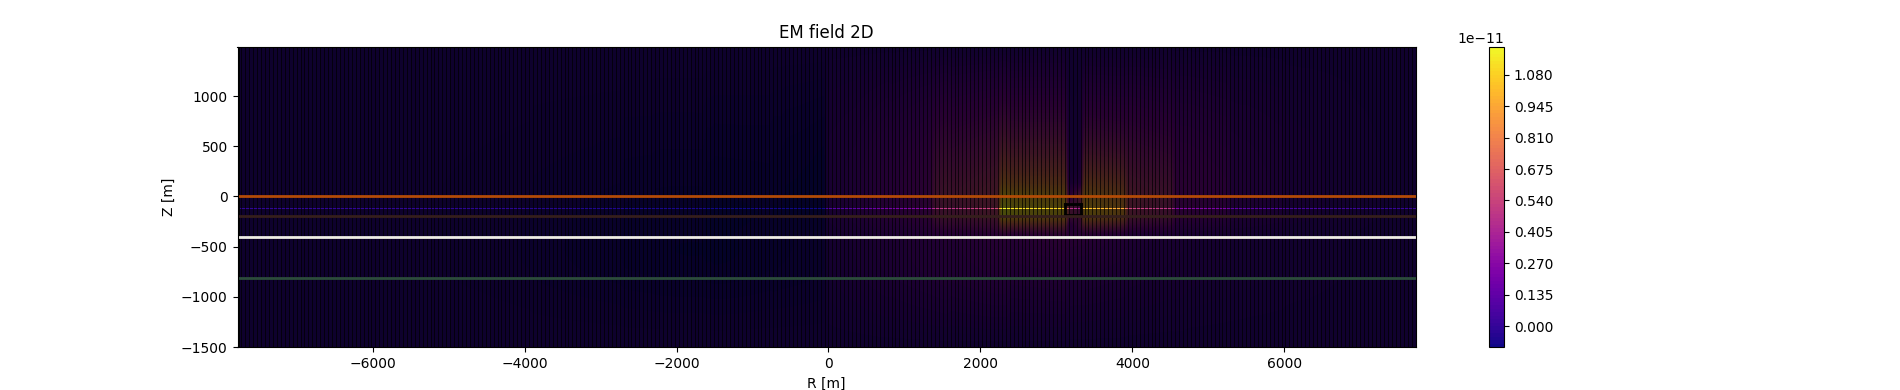
\includegraphics[width=1.0\linewidth]{images/Answer_A_Istage_time_layer_1.0250000000000006.png}
	\caption{Решение суммарного поля $\overrightarrow{\textbf{A}}$ при $t = 1.025с$}
	\label{fig:A_Istage_t1}
\end{figure} 


\begin{figure}
	\centering
	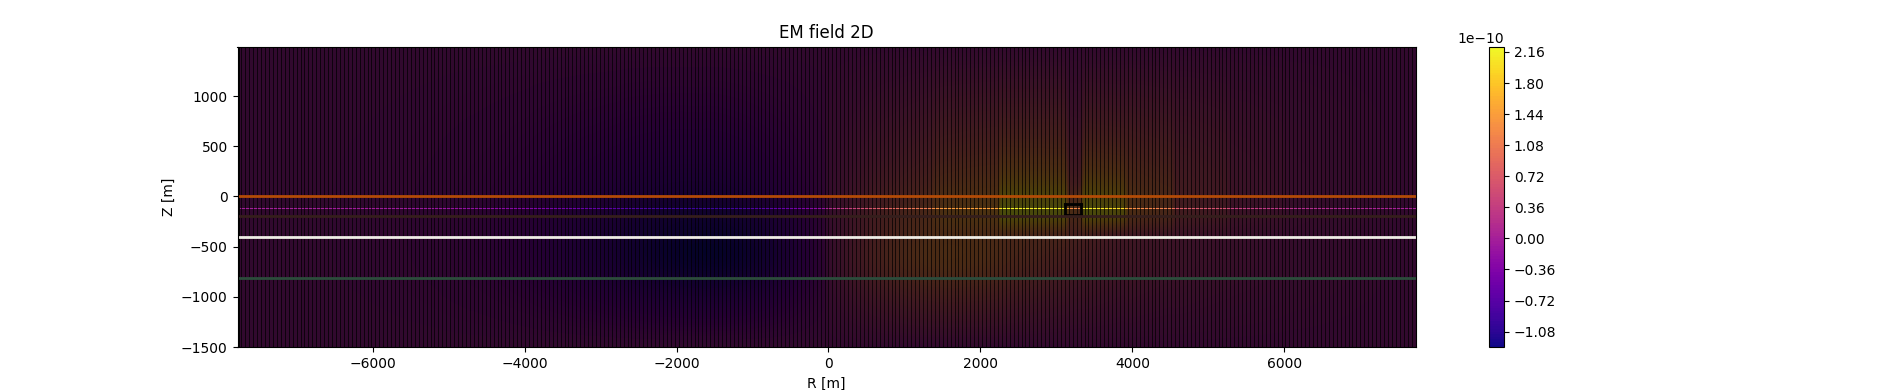
\includegraphics[width=1.0\linewidth]{images/Answer_E_Istage_time_layer_1.0250000000000006.png}
	\caption{Решение суммарного поля $\overrightarrow{\textbf{E}}$ при $t = 1.025с$}
	\label{fig:E_Istage_t1}
\end{figure} 

\begin{figure}
	\centering
	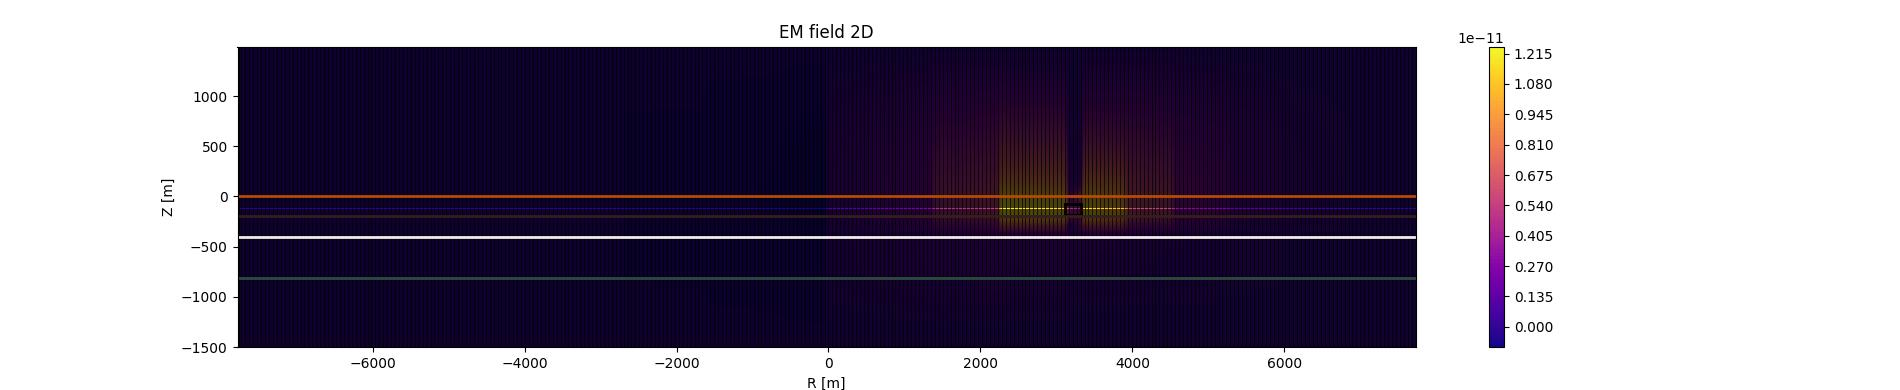
\includegraphics[width=1.0\linewidth]{images/Answer_A_Istage_time_layer_1.05.png}
	\caption{Решение суммарного поля $\overrightarrow{\textbf{A}}$ при $t = 1.05с$}
	\label{fig:A_Istage_t2}
\end{figure} 


\begin{figure}
	\centering
	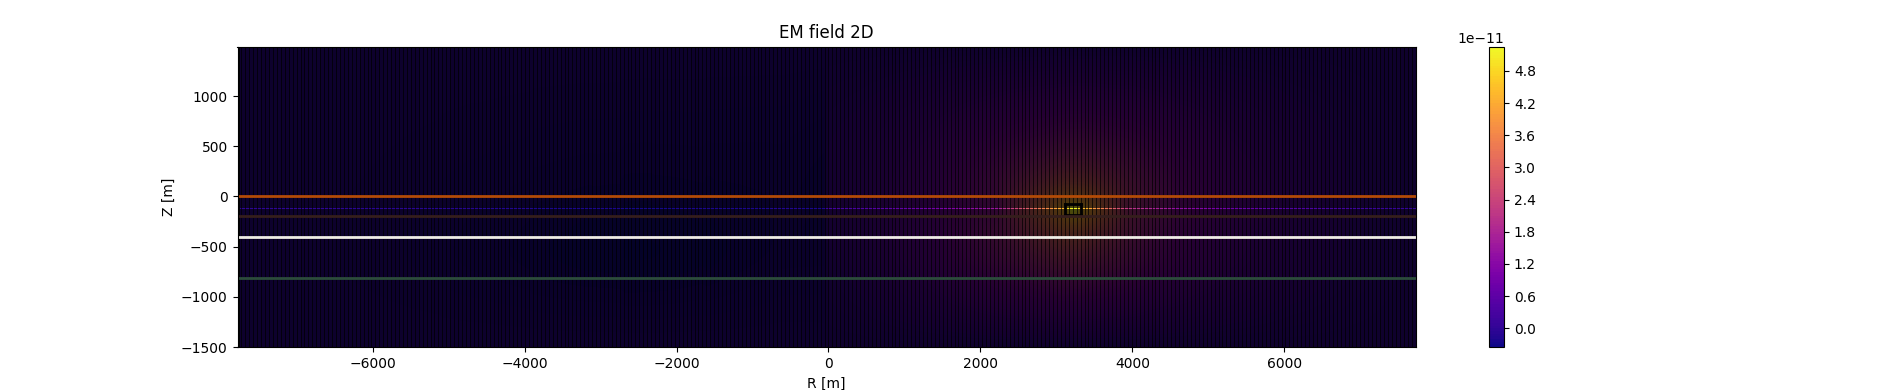
\includegraphics[width=1.0\linewidth]{images/Answer_E_Istage_time_layer_1.05.png}
	\caption{Решение суммарного поля $\overrightarrow{\textbf{E}}$ при $t = 1.05с$}
	\label{fig:E_Istage_t2}
\end{figure} 

Полученные значения \ref{fig:A_Log_added} -- \ref{fig:E_Log_added} $\overrightarrow{\textbf{A}}$ и $\overrightarrow{\textbf{E}}$ рассмотрим на приёмниках.

\begin{figure}
	\centering
	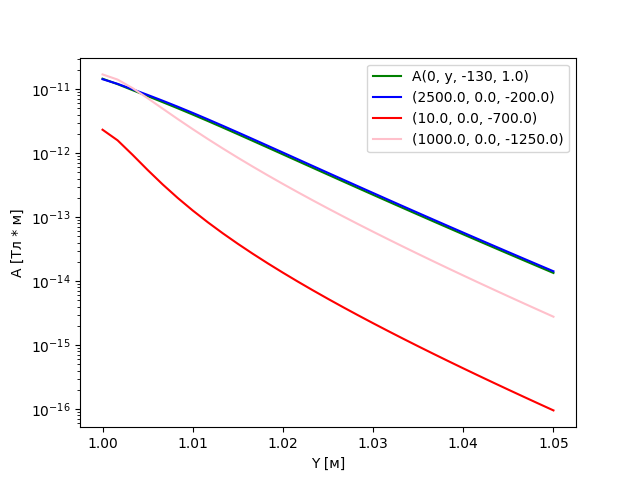
\includegraphics[width=0.8\linewidth]{images/Log_A_obj1.png}
	\caption{Решение суммарного поля $\overrightarrow{\textbf{E}}$ при $t = 1.05с$}
	\label{fig:A_Log_added}
\end{figure} 


\begin{figure}
	\centering
	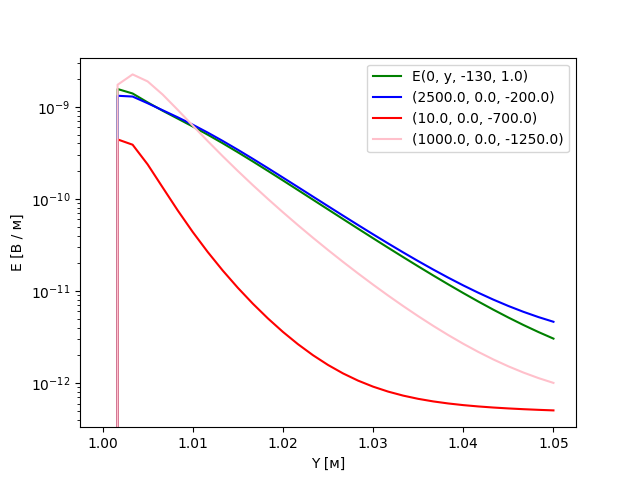
\includegraphics[width=0.8\linewidth]{images/Log_E_obj1.png}
	\caption{Решение суммарного поля $\overrightarrow{\textbf{E}}$ при $t = 1.05с$}
	\label{fig:E_Log_added}
\end{figure} 

Сравнивая показатели на приёмниках до добавления аномалии \ref{fig:LogA} -- \ref{fig:LogE} и после \ref{fig:A_Log_added} -- \ref{fig:A_Log_added}, можно заметить, что значения напряжённости электрического поля на красном приёмнике претерпели наиболее сильные изменения, т.к. он стал более похожим на гиперболу, нежели прямую линию. Значения на синем приёмнике начали изменяться уже в последние сотые секунды исследования. 

\section{Исследование многоэтапного разделения нормального и добавочных полей}

Добавим ещё один аномальный объект со следующими границами: $[-1305; -1050]_x \times [-2255; -2178]_y \times [-1250; -800]_z$ и значением $\sigma = 17$. Будем искать решение из уравнения на добавочное поле (\ref{eq_1_6}). Получим решения в разные моменты времени изображенные на рисунках \ref{fig:A_2plus_t0} -- \ref{fig:E_2plus_t2}.

\begin{figure}
	\centering
	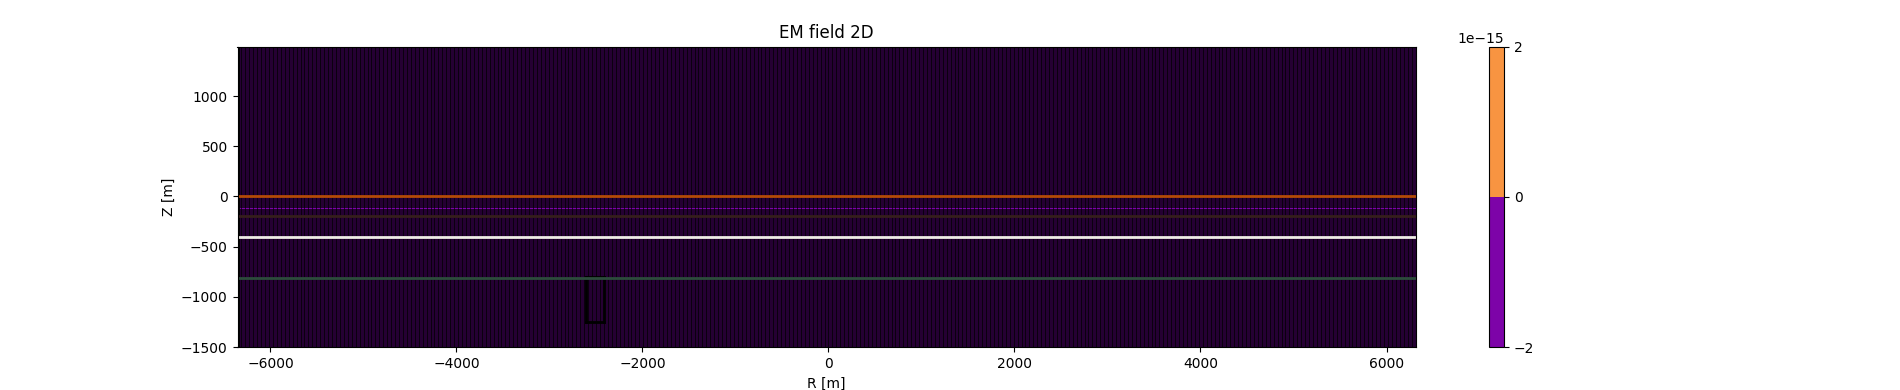
\includegraphics[width=1.0\linewidth]{images/Answer_A_2plus_time_layer_1.png}
	\caption{Решение $\overrightarrow{\textbf{A}}^+$ при $t = 1.0с$}
	\label{fig:A_2plus_t0}
\end{figure} 


\begin{figure}
	\centering
	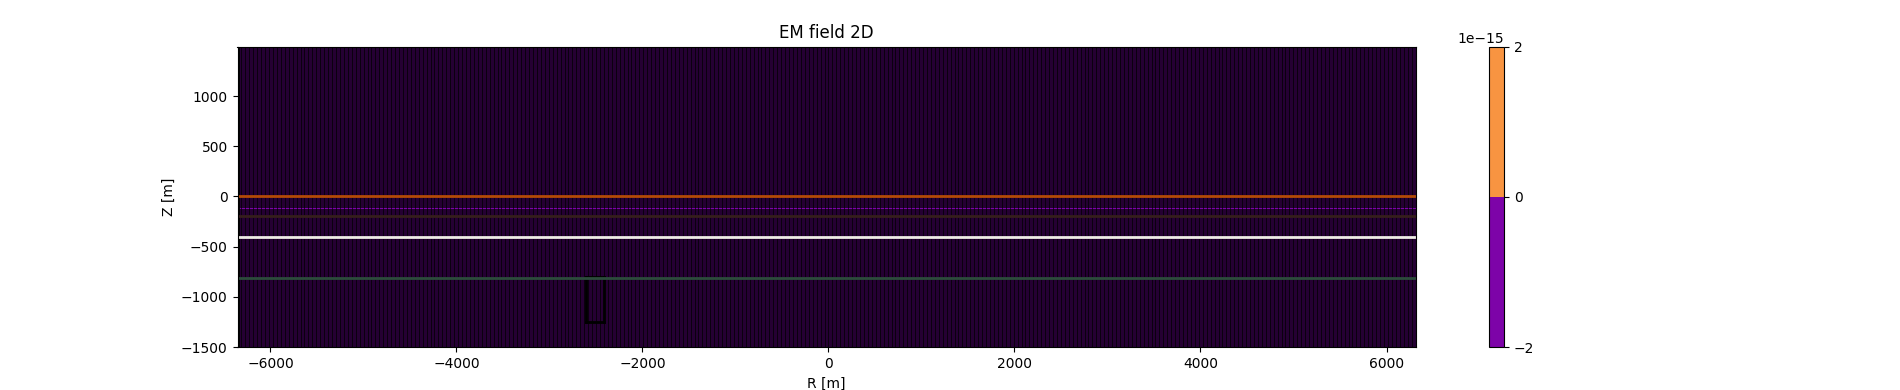
\includegraphics[width=1.0\linewidth]{images/Answer_E_2plus_time_layer_1.png}
	\caption{Решение $\overrightarrow{\textbf{E}}^+$ при $t = 1.0с$}
	\label{fig:E_2plus_t0}
\end{figure} 


\begin{figure}
	\centering
	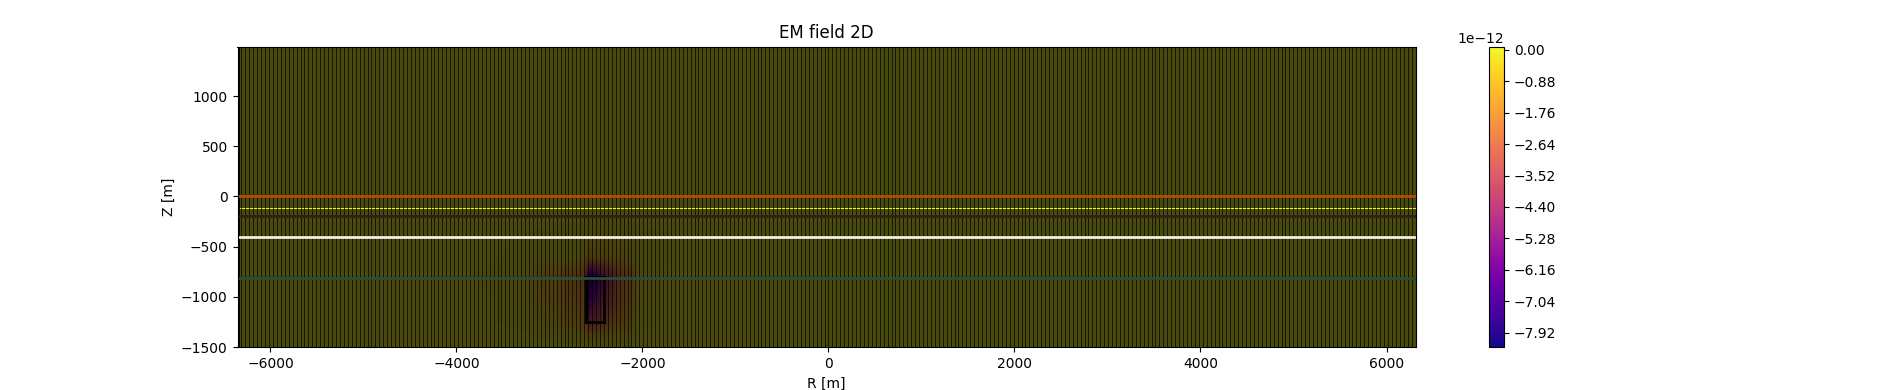
\includegraphics[width=1.0\linewidth]{images/Answer_A_2plus_time_layer_1.0250000000000006.png}
	\caption{Решение $\overrightarrow{\textbf{A}}^+$ при $t = 1.025с$}
	\label{fig:A_2plus_t1}
\end{figure} 


\begin{figure}
	\centering
	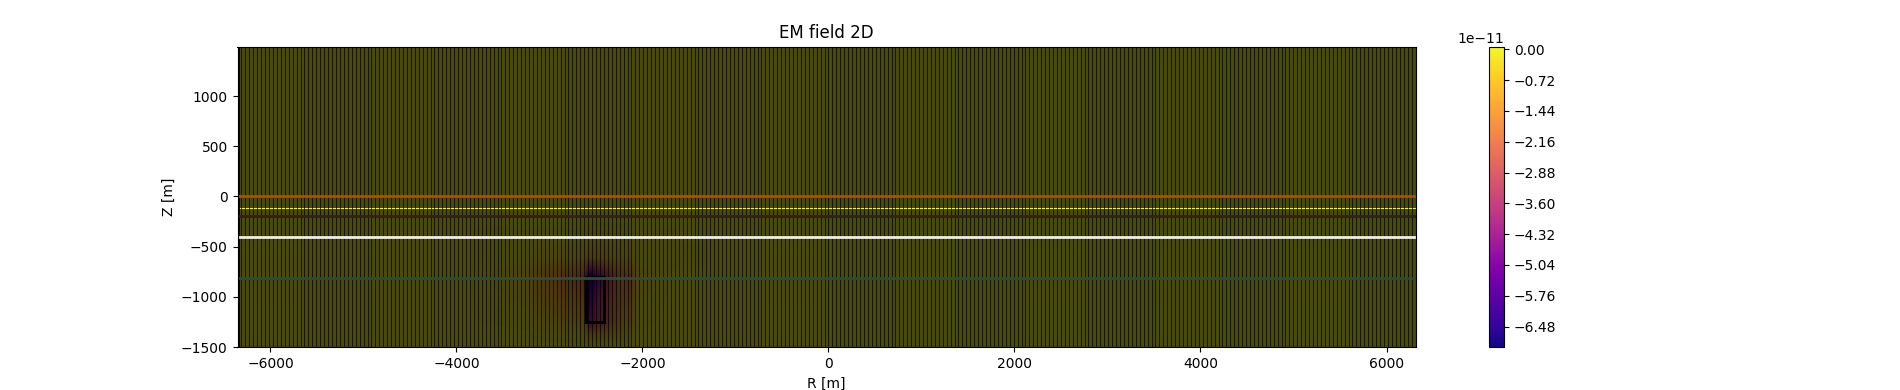
\includegraphics[width=1.0\linewidth]{images/Answer_E_2plus_time_layer_1.0250000000000006.png}
	\caption{Решение $\overrightarrow{\textbf{E}}^+$ при $t = 1.025с$}
	\label{fig:E_2plus_t1}
\end{figure} 

\begin{figure}
	\centering
	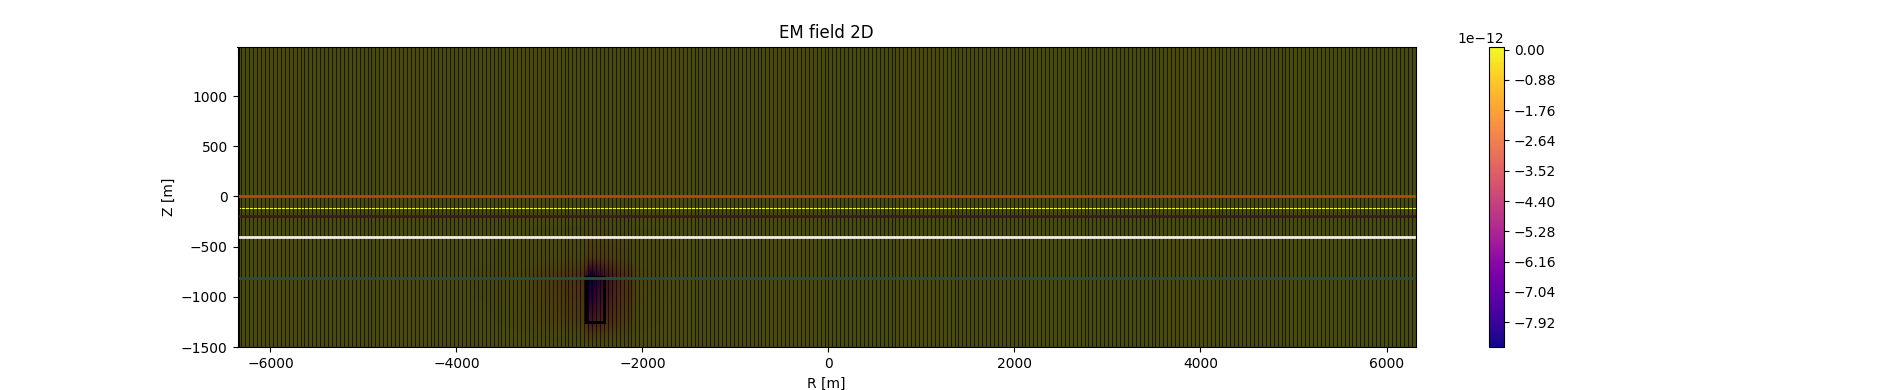
\includegraphics[width=1.0\linewidth]{images/Answer_A_2plus_time_layer_1.05.png}
	\caption{Решение $\overrightarrow{\textbf{A}}^+$ при $t = 1.05с$}
	\label{fig:A_2plus_t2}
\end{figure} 


\begin{figure}
	\centering
	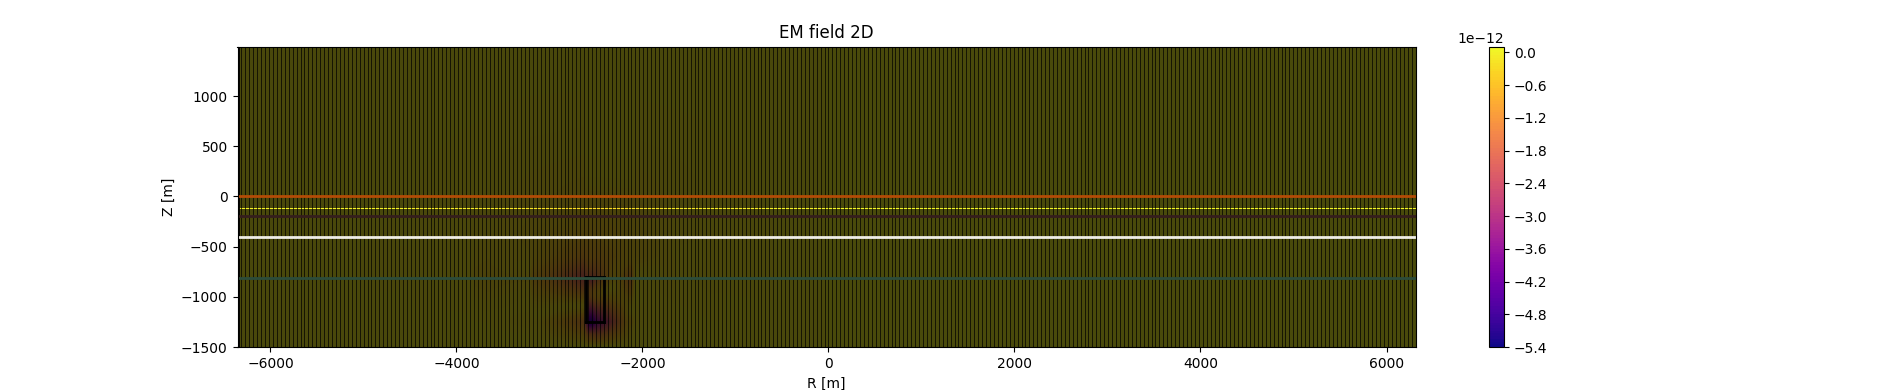
\includegraphics[width=1.0\linewidth]{images/Answer_E_2plus_time_layer_1.05.png}
	\caption{Решение $\overrightarrow{\textbf{E}}^+$ при $t = 1.05с$}
	\label{fig:E_2plus_t2}
\end{figure} 

Рассмотрим для $t = 1.0, t = 1.025, t = 1.05$ значения $\overrightarrow{\textbf{A}}^+$ и $\overrightarrow{\textbf{E}}^+$ на линии, перпендикулярно проходящей к аномальному объекту по оси $y$ при $x = -1177.5, z = -1050.0$. Получим следующее:

\begin{figure}
	\centering
	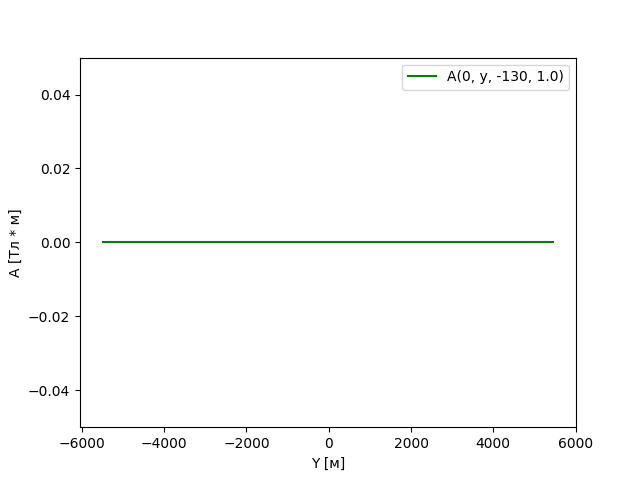
\includegraphics[width=0.5\linewidth]{images/Normal_A_obj2_1.png}
	\caption{Решение $\overrightarrow{\textbf{A}}$ на линии $(0.0, y, -130.0)$ при $t = 1.025с$}
	\label{fig:A_2line_t0}
\end{figure} 

\begin{figure}
	\centering
	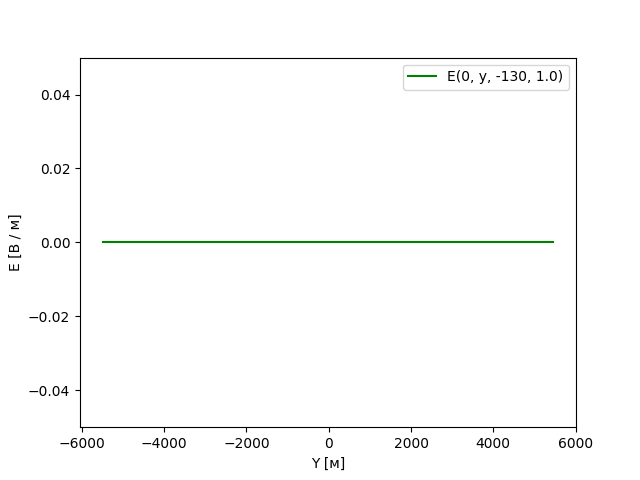
\includegraphics[width=0.5\linewidth]{images/Normal_E_obj2_1.png}
	\caption{Решение $\overrightarrow{\textbf{E}}$ на линии $(0.0, y, -130.0)$ при $t = 1.025с$}
	\label{fig:E_2line_t0}
\end{figure} 

\begin{figure}
	\centering
	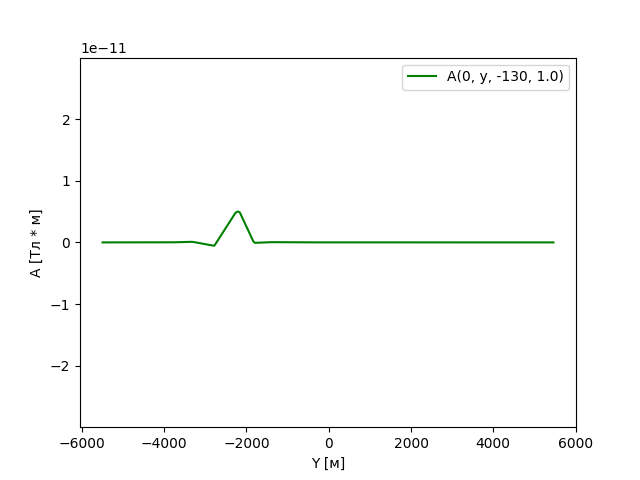
\includegraphics[width=0.5\linewidth]{images/Normal_A_obj2_2.png}
	\caption{Решение $\overrightarrow{\textbf{A}}$ на линии $(0.0, y, -130.0)$ при $t = 1.025с$}
	\label{fig:A_2line_t1}
\end{figure} 

\begin{figure}
	\centering
	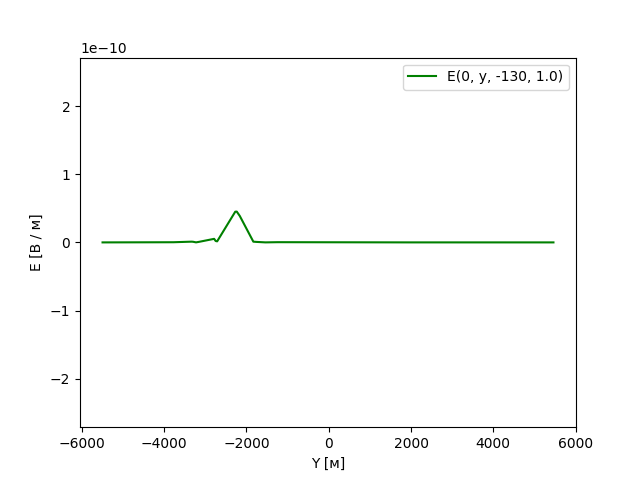
\includegraphics[width=0.5\linewidth]{images/Normal_E_obj2_2.png}
	\caption{Решение $\overrightarrow{\textbf{E}}$ на линии $(0.0, y, -130.0)$  при $t = 1.025с$}
	\label{fig:E_2line_t1}
\end{figure} 

\begin{figure}
	\centering
	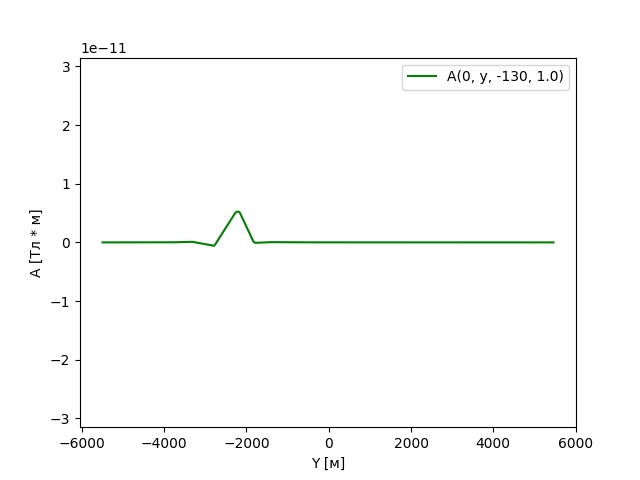
\includegraphics[width=0.5\linewidth]{images/Normal_A_obj2_3.png}
	\caption{Решение $\overrightarrow{\textbf{A}}$ на линии $(0.0, y, -130.0)$  при $t = 1.05с$}
	\label{fig:A_2line_t2}
\end{figure} 

\begin{figure}
	\centering
	\includegraphics[width=0.5\linewidth]{images/Normal_E_obj2_2.png}
	\caption{Решение $\overrightarrow{\textbf{A}}$ на линии $(0.0, y, -130.0)$  при $t = 1.05с$}
	\label{fig:E_2line_t2}
\end{figure} 

Суммируем полученный результат с полем без аномалий и получим состояние поля в разные моменты времени, изображённые на рисунках \ref{fig:A_IIstage_t0} -- \ref{fig:E_IIstage_t2}.

\begin{figure}
	\centering
	\includegraphics[width=1.0\linewidth]{images/Answer_A_IIstage_time_layer_1.png}
	\caption{Решение суммарного поля $\overrightarrow{\textbf{A}}$ при $t = 1.0с$}
	\label{fig:A_IIstage_t0}
\end{figure} 


\begin{figure}
	\centering
	\includegraphics[width=1.0\linewidth]{images/Answer_E_IIstage_time_layer_1.png}
	\caption{Решение суммарного поля $\overrightarrow{\textbf{E}}$ при $t = 1.0с$}
	\label{fig:E_IIstage_t0}
\end{figure} 


\begin{figure}
	\centering
	\includegraphics[width=1.0\linewidth]{images/Answer_A_IIstage_time_layer_1.0250000000000006.png}
	\caption{Решение суммарного поля $\overrightarrow{\textbf{A}}$ при $t = 1.025с$}
	\label{fig:A_IIstage_t1}
\end{figure} 


\begin{figure}
	\centering
	\includegraphics[width=1.0\linewidth]{images/Answer_E_IIstage_time_layer_1.0250000000000006.png}
	\caption{Решение суммарного поля $\overrightarrow{\textbf{E}}$ при $t = 1.025с$}
	\label{fig:E_IIstage_t1}
\end{figure} 

\begin{figure}
	\centering
	\includegraphics[width=1.0\linewidth]{images/Answer_A_IIstage_time_layer_1.05.png}
	\caption{Решение суммарного поля $\overrightarrow{\textbf{A}}$ при $t = 1.05с$}
	\label{fig:A_IIstage_t2}
\end{figure} 


\begin{figure}
	\centering
	\includegraphics[width=1.0\linewidth]{images/Answer_E_IIstage_time_layer_1.05.png}
	\caption{Решение суммарного поля $\overrightarrow{\textbf{E}}$ при $t = 1.05с$}
	\label{fig:E_IIstage_t2}
\end{figure} 

Полученные значения \ref{fig:A_Log_added2} -- \ref{fig:E_Log_added2} $\overrightarrow{\textbf{A}}$ и $\overrightarrow{\textbf{E}}$ рассмотрим на приёмниках.

\begin{figure}
	\centering
	\includegraphics[width=0.8\linewidth]{images/Log_A_obj2.png}
	\caption{Решение суммарного поля $\overrightarrow{\textbf{E}}$ при $t = 1.05с$}
	\label{fig:A_Log_added2}
\end{figure} 


\begin{figure}
	\centering
	\includegraphics[width=0.8\linewidth]{images/Log_E_obj2.png}
	\caption{Решение суммарного поля $\overrightarrow{\textbf{E}}$ при $t = 1.05с$}
	\label{fig:E_Log_added2}
\end{figure} 

Сравнивая показатели на приёмниках до добавления аномалии \ref{fig:LogA} -- \ref{fig:LogE} и после \ref{fig:A_Log_added2} -- \ref{fig:A_Log_added2}, можно заметить, что значения напряжённости электрического поля ни на одном из приёмников не претерпели изменения, по всей видимости из-за неудачного их расположения. Для изменения ситуации необходимо было бы увеличить размеры расчётной области по пространству и временного диапазона. 

Рассмотрим теперь поле с двумя объектами сразу. Для этого сначала добавим первый объект к чистой расчётной области, после используя его в качестве нормального, добавим вторую аномалию.

\begin{figure}
	\centering
	\includegraphics[width=1.0\linewidth]{images/Answer_A_both_time_layer_1.png}
	\caption{Решение суммарного поля $\overrightarrow{\textbf{A}}$ при $t = 1.0с$}
	\label{fig:A_both_t0}
\end{figure} 


\begin{figure}
	\centering
	\includegraphics[width=1.0\linewidth]{images/Answer_E_both_time_layer_1.png}
	\caption{Решение суммарного поля $\overrightarrow{\textbf{E}}$ при $t = 1.0с$}
	\label{fig:E_both_t0}
\end{figure} 


\begin{figure}
	\centering
	\includegraphics[width=1.0\linewidth]{images/Answer_A_both_time_layer_1.0250000000000006.png}
	\caption{Решение суммарного поля $\overrightarrow{\textbf{A}}$ при $t = 1.025с$}
	\label{fig:A_both_t1}
\end{figure} 


\begin{figure}
	\centering
	\includegraphics[width=1.0\linewidth]{images/Answer_E_both_time_layer_1.0250000000000006.png}
	\caption{Решение суммарного поля $\overrightarrow{\textbf{E}}$ при $t = 1.025с$}
	\label{fig:E_both_t1}
\end{figure} 

\begin{figure}
	\centering
	\includegraphics[width=1.0\linewidth]{images/Answer_A_both_time_layer_1.05.png}
	\caption{Решение суммарного поля $\overrightarrow{\textbf{A}}$ при $t = 1.05с$}
	\label{fig:A_both_t2}
\end{figure} 


\begin{figure}
	\centering
	\includegraphics[width=1.0\linewidth]{images/Answer_E_both_time_layer_1.05.png}
	\caption{Решение суммарного поля $\overrightarrow{\textbf{E}}$ при $t = 1.05с$}
	\label{fig:E_both_t2}
\end{figure} 

Полученные значения \ref{fig:A_Log_both} -- \ref{fig:E_Log_both} $\overrightarrow{\textbf{A}}$ и $\overrightarrow{\textbf{E}}$ рассмотрим на приёмниках.

\begin{figure}
	\centering
	\includegraphics[width=0.8\linewidth]{images/Log_A_both.png}
	\caption{Решение суммарного поля $\overrightarrow{\textbf{E}}$ при $t = 1.05с$}
	\label{fig:A_Log_both}
\end{figure} 


\begin{figure}
	\centering
	\includegraphics[width=0.8\linewidth]{images/Log_E_both.png}
	\caption{Решение суммарного поля $\overrightarrow{\textbf{E}}$ при $t = 1.05с$}
	\label{fig:E_Log_both}
\end{figure} 

Сравнивая показатели на приёмниках до добавления обеих аномалий \ref{fig:LogA} -- \ref{fig:LogE} и после \ref{fig:A_Log_both} -- \ref{fig:E_Log_both}, можно заметить, что значения напряжённости электрического поля на красном приёмнике все те же изменения, что и без учёта второго объекта. Это связано со слабым влиянием второго объекта на приёмники. 
\chapter*{Заключение}

\addcontentsline{toc}{chapter}{Заключение}


Мир, в котором мы живем, состоит из разнообразных регионов, каждый из которых имеет уникальный набор проблем и проблем. Эти региональные проблемы могут варьироваться от экологических проблем, таких как загрязнение и изменение климата, до социальных и экономических проблем, таких как бедность и безработица. Решение этих проблем имеет решающее значение для устойчивого развития и благополучия затронутых регионов и их жителей.

\newpage

\addcontentsline{toc}{chapter}{Список используемых источников}
\renewcommand\bibname{СПИСОК ИСПОЛЬЗУЕМЫХ ИСТОЧНИКОВ}

\begin{thebibliography}{00}
	\bibitem{1}
			М.С. Жданов Электроразведка. - М.: Недра, 1986. - 316 с.
    \bibitem{2}
			А.А. Логачев, В.П. Захаров Магниторазведка. - 5 изд. - Ленинград: Недра, 1979. - 350 с.
    \bibitem{3}
    		Pavel Solin Partial Differential Equations and the Finite Element Method. - Hoboken, New Jersey: A JOHN WILEY $\&$ SONS, INC., 2006.
    \bibitem{4}
    		А.Н. Тихонов, А.А. Самарский Уравнения математической физики: Учеб.пособие. / А.Н. Тихонов, А.А. Самарский — 6-е изд., — М: Изд-во МГУ, 1999 — 799 с.
   	\bibitem{5}		
 			М.Г. Персова, Ю.Г. Соловейчик, М.Г. Токарева, М.В. Абрамов 3D-моделирование процессов индукционной вызванной поляризации при возбуждении токовой петлей и проблема эквивалентности // Научный вестник НГТУ. - 2013. - №2(51). - С. 53 - 61.
    \bibitem{6}
   			М. Г. Персова, Ю. Г. Соловейчик, Г. М. Тригубович, М. В. Абрамов, А. А. Заборцева О вычислении трёхмерного нестационарного поля вертикальной электрической линии в удалённой обсаженной скважине // Сибирский журнал индустриальной математики. - 2007. - №3(31). - С. 114 - 127.
    \bibitem{7}
			Ю.Г. Соловейчик, М.Э. Рояк, М.Г. Персова Метод конечных элементов для скалярных и векторных задач Учеб. пособие. — Новосибирск: Изд-во НГТУ, 2007 — 896 с.
	\bibitem{8}
			М.Ю.Баландин, Э.П.Шурина Векторный метод конечных элементов: Учеб. пособие. - Новосибирск: Изд-во НГТУ, 2001 — 69 с.
	\bibitem{9}
  			М.Ю.Баландин, Э.П.Шурина Методы решения СЛАУ большой размерности: Учеб. пособие. - Новосибирск: Изд-во НГТУ, 2000 — 70 с.
	\bibitem{10}
    		М.Г. Персова, Ю.Г. Соловейчик, Д.В. Вагин, П.А. Домников, Ю.И. Кошкина Численные методы в уравнениях математической физики.  - Новосибирск: Изд-во НГТУ, 2016 — 60 с.
    \bibitem{11}
    		Вагин Денис Владимирович Разработка методов конечноэлементного моделирования трехмерных электромагнитных полей на неструктурированных сетках: автореф. дис. канд. техн. наук: 05.13.18. - Новосибирск, 2012.
    \bibitem{12}	
    		Тракимус Юрий Викторович Разработка и применение схем конечноэлементного моделирования электромагнитных полей в задачах электроразведки с использованием скважин: автореф. дис. канд. техн. наук: 05.13.18. - Новосибирск, 2007.
    \bibitem{13}
    		П.А. Домников Решение систем конечноэлементных уравнений при моделировании гармонических геоэлектромагнитных полей в трехмерных задачах морской электроразведки // Доклады Академии наук высшей школы Российской Федерации. - 2013. - №1 (20).
\end{thebibliography}

\newpage
%\hypertarget{a1}{}
\chapter*{Приложение 1. Тестирование двумерной задачи на полиномах}
\addcontentsline{toc}{chapter}{Приложение 1. Тестирование двумерной задачи на полиномах}

Проведем сначала тестирование программы на работоспособность для уравнения (\ref{eq_4_1}). Образец расчетной области изображен на рисунке \ref{fig:exampleOf3DMesh}. Это область $\Omega = [1.0, 2.0]_r \times [1.0, 2.0]_z$, она содержит 16 узлов, а на всех границах будем задавать первые краевые условия.

\begin{equation} \label{eq_4_1}
	-\frac{1}{\mu_0 r} \frac{\partial}{\partial r} \left(r \frac{\partial u}{\partial r}\right) - \frac{1}{\mu_0} \frac{\partial^2 u}{\partial z^2} + \frac{u}{\mu_0 r^2} + \sigma \frac{\partial A_{\varphi}}{\partial t} = f,
\end{equation}

\begin{figure}
	\centering
	\includegraphics[width=0.75\linewidth]{images/"TestMesh".png}
	\caption{Расчетная область}
	\label{fig:exampleOf3DMesh}
\end{figure}

\begin{table}
	\caption{Тестирование при $u = 2$, $f = \frac{2}{r^2}$, $\mu_0 = 1,\sigma = 0$}
	\centering
	\small
	\begin{tabularx}{1.0\textwidth}{| >{\raggedright\arraybackslash}X | >{\raggedright\arraybackslash}X | >{\raggedright\arraybackslash}X |>{\raggedright\arraybackslash}X |}
		\hline
		\centering{Узел} & \centering{Значение} & \centering{Абсолютная погрешность} & \centering{Относительная погрешность} \tabularnewline \hline
		
		
		
		\centering{(${}^4/_3$; ${}^4/_3$)} & \centering{2.00226896E+000}& \centering{2.26896083E-003} & \centering{1.13448042E-003} \tabularnewline \hline
		
		\centering{(${}^5/_3$; ${}^4/_3$)} & \centering{2.00130487E+000} & \centering{1.30486533E-003} & \centering{6.52432666E-004} \tabularnewline \hline
		
		\centering{(${}^4/_3$; ${}^5/_3$)} & \centering{2.00226896E+000} & \centering{2.26896083E-003} & \centering{1.13448042E-003} \tabularnewline \hline
		
		\centering{(${}^5/_3$; ${}^5/_3$)} & \centering{2.00130487E+000} & \centering{1.30486533E-003} & \centering{6.52432666E-004} \tabularnewline \hline
		
	\end{tabularx}
	\label{tab:test1}
\end{table}

\begin{table}
	\caption{Тестирование при $u = r$, $f = 0$, $\mu_0 = 1,\sigma = 0$}
	\centering
	\small
	\begin{tabularx}{1.0\textwidth}{| >{\raggedright\arraybackslash}X | >{\raggedright\arraybackslash}X | >{\raggedright\arraybackslash}X |>{\raggedright\arraybackslash}X |}
		\hline
		\centering{Узел} & \centering{Значение} & \centering{Абсолютная погрешность} & \centering{Относительная погрешность} \tabularnewline \hline
		
		
		
		\centering{(${}^4/_3$; ${}^4/_3$)} & \centering{1.33333333E+000}& \centering{1.33226763E-015} & \centering{9.99200722E-016} \tabularnewline \hline
		
		\centering{(${}^5/_3$; ${}^4/_3$)} & \centering{1.66666667E+000} & \centering{6.66133815E-016} & \centering{3.99680289E-016} \tabularnewline \hline
		
		\centering{(${}^4/_3$; ${}^5/_3$)} & \centering{1.33333333E+000} & \centering{1.77635684E-015} & \centering{1.33226763E-015} \tabularnewline \hline
		
		\centering{(${}^5/_3$; ${}^5/_3$)} & \centering{1.66666667E+000} & \centering{6.66133815E-016} & \centering{3.99680289E-016} \tabularnewline \hline
		
	\end{tabularx}
	\label{tab:test2}
\end{table}

\begin{table}
	\caption{Тестирование при $u = z$, $f = \frac{z}{r^2}$, $\mu_0 = 1,\sigma = 0$}
	\centering
	\small
	\begin{tabularx}{1.0\textwidth}{| >{\raggedright\arraybackslash}X | >{\raggedright\arraybackslash}X | >{\raggedright\arraybackslash}X |>{\raggedright\arraybackslash}X |}
		\hline
		\centering{Узел} & \centering{Значение} & \centering{Абсолютная погрешность} & \centering{Относительная погрешность} \tabularnewline \hline
		
		
		
		\centering{(${}^4/_3$; ${}^4/_3$)} & \centering{1.33491362E+000}& \centering{1.58028263E-003} & \centering{1.18521198E-003} \tabularnewline \hline
		
		\centering{(${}^5/_3$; ${}^4/_3$)} & \centering{1.33426439E+000} & \centering{9.31054340E-004} & \centering{6.98290755E-004} \tabularnewline \hline
		
		\centering{(${}^4/_3$; ${}^5/_3$)} & \centering{1.66848983E+000} & \centering{1.82315862E-003} & \centering{1.09389517E-003} \tabularnewline \hline
		
		\centering{(${}^5/_3$; ${}^5/_3$)} & \centering{1.66769291E+000} & \centering{1.02624366E-003} & \centering{6.15746195E-004} \tabularnewline \hline
		
	\end{tabularx}
	\label{tab:test3}
\end{table}

\begin{table}
	\caption{Тестирование при $u = r+z$, $f = \frac{z}{r^2}$, $\mu_0 = 1,\sigma = 0$}
	\centering
	\small
	\begin{tabularx}{1.0\textwidth}{| >{\raggedright\arraybackslash}X | >{\raggedright\arraybackslash}X | >{\raggedright\arraybackslash}X |>{\raggedright\arraybackslash}X |}
		\hline
		\centering{Узел} & \centering{Значение} & \centering{Абсолютная погрешность} & \centering{Относительная погрешность} \tabularnewline \hline
		
		
		
		\centering{(${}^4/_3$; ${}^4/_3$)} & \centering{2.66824695E+000}& \centering{1.58028263E-003} & \centering{5.92605988E-004} \tabularnewline \hline
		
		\centering{(${}^5/_3$; ${}^4/_3$)} & \centering{3.00093105E+000} & \centering{9.31054340E-004} & \centering{3.10351447E-004} \tabularnewline \hline
		
		\centering{(${}^4/_3$; ${}^5/_3$)} & \centering{3.00182316E+000} & \centering{1.82315862E-003} & \centering{6.07719539E-004} \tabularnewline \hline
		
		\centering{(${}^5/_3$; ${}^5/_3$)} & \centering{3.33435958E+000} & \centering{1.02624366E-003} & \centering{3.07873097E-004} \tabularnewline \hline
		
	\end{tabularx}
	\label{tab:test4}
\end{table}

\begin{table}
	\caption{Тестирование при $u = rz$, $f = 0$, $\mu_0 = 1,\sigma = 0$}
	\centering
	\small
	\begin{tabularx}{1.0\textwidth}{| >{\raggedright\arraybackslash}X | >{\raggedright\arraybackslash}X | >{\raggedright\arraybackslash}X |>{\raggedright\arraybackslash}X |}
		\hline
		\centering{Узел} & \centering{Значение} & \centering{Абсолютная погрешность} & \centering{Относительная погрешность} \tabularnewline \hline
		
		
		
		\centering{(${}^4/_3$; ${}^4/_3$)} & \centering{1.77777778E+000}& \centering{1.11022302E-015} & \centering{6.24500451E-016} \tabularnewline \hline
		
		\centering{(${}^5/_3$; ${}^4/_3$)} & \centering{2.22222222E+000} & \centering{3.10862447E-015} & \centering{1.39888101E-015} \tabularnewline \hline
		
		\centering{(${}^4/_3$; ${}^5/_3$)} & \centering{2.22222222E+000} & \centering{8.88178420E-016} & \centering{3.99680289E-016} \tabularnewline \hline
		
		\centering{(${}^5/_3$; ${}^5/_3$)} & \centering{2.77777778E+000} & \centering{4.88498131E-015} & \centering{1.75859327E-015} \tabularnewline \hline
		
	\end{tabularx}
	\label{tab:test5}
\end{table}

\begin{table}
	\caption{Тестирование при $u = r^2 + z^2$, $f = \frac{z^2}{r^2} - 5$, $\mu_0 = 1,\sigma = 0$}
	\centering
	\small
	\begin{tabularx}{1.0\textwidth}{| >{\raggedright\arraybackslash}X | >{\raggedright\arraybackslash}X | >{\raggedright\arraybackslash}X |>{\raggedright\arraybackslash}X |}
		\hline
		\centering{Узел} & \centering{Значение} & \centering{Абсолютная погрешность} & \centering{Относительная погрешность} \tabularnewline \hline
		
		
		
		\centering{(${}^4/_3$; ${}^4/_3$)} & \centering{3.55717205E+000}& \centering{1.61649660E-003} & \centering{4.54639669E-004} \tabularnewline \hline
		
		\centering{(${}^5/_3$; ${}^4/_3$)} & \centering{4.55644336E+000} & \centering{8.87803368E-004} & \centering{1.94883666E-004} \tabularnewline \hline
		
		\centering{(${}^4/_3$; ${}^5/_3$)} & \centering{4.55790068E+000} & \centering{2.34512455E-003} & \centering{5.14783438E-004} \tabularnewline \hline
		
		\centering{(${}^5/_3$; ${}^5/_3$)} & \centering{5.55672893E+000} & \centering{1.17337132E-003} & \centering{2.11206838E-004} \tabularnewline \hline
		
	\end{tabularx}
	\label{tab:test6}
\end{table}

\begin{table}
	\caption{Тестирование при $u = r^2 z^2$, $f = -3z^2 - 2r^2$, $\mu_0 = 1,\sigma = 0$}
	\centering
	\small
	\begin{tabularx}{1.0\textwidth}{| >{\raggedright\arraybackslash}X | >{\raggedright\arraybackslash}X | >{\raggedright\arraybackslash}X |>{\raggedright\arraybackslash}X |}
		\hline
		\centering{Узел} & \centering{Значение} & \centering{Абсолютная погрешность} & \centering{Относительная погрешность} \tabularnewline \hline
		
		
		
		\centering{(${}^4/_3$; ${}^4/_3$)} & \centering{3.15919390E+000}& \centering{1.29993140E-003} & \centering{4.11306418E-004} \tabularnewline \hline
		
		\centering{(${}^5/_3$; ${}^4/_3$)} & \centering{4.93728492E+000} & \centering{9.86688136E-004} & \centering{1.99804348E-004} \tabularnewline \hline
		
		\centering{(${}^4/_3$; ${}^5/_3$)} & \centering{4.93658403E+000} & \centering{1.68757555E-003} & \centering{3.41734049E-004} \tabularnewline \hline
		
		\centering{(${}^5/_3$; ${}^5/_3$)} & \centering{7.71481536E+000} & \centering{1.23402231E-003} & \centering{1.59929291E-004} \tabularnewline \hline
		
	\end{tabularx}
	\label{tab:test7}
\end{table}

\begin{table}
	\caption{Тестирование при $u = r^3+z^3$, $f = -8r -6z + \frac{z^3}{r^2}$, $\mu_0 = 1,\sigma = 0$}
	\centering
	\small
	\begin{tabularx}{1.0\textwidth}{| >{\raggedright\arraybackslash}X | >{\raggedright\arraybackslash}X | >{\raggedright\arraybackslash}X |>{\raggedright\arraybackslash}X |}
		\hline
		\centering{Узел} & \centering{Значение} & \centering{Абсолютная погрешность} & \centering{Относительная погрешность} \tabularnewline \hline
		
		
		
		\centering{(${}^4/_3$; ${}^4/_3$)} & \centering{4.73874864E+000}& \centering{1.99210278E-003} & \centering{4.20209180E-004} \tabularnewline \hline
		
		\centering{(${}^5/_3$; ${}^4/_3$)} & \centering{6.99757994E+000} & \centering{2.42006018E-003} & \centering{3.45722883E-004} \tabularnewline \hline
		
		\centering{(${}^4/_3$; ${}^5/_3$)} & \centering{6.99968104E+000} & \centering{3.18957115E-004} & \centering{4.55653022E-005} \tabularnewline \hline
		
		\centering{(${}^5/_3$; ${}^5/_3$)} & \centering{9.25749495E+000} & \centering{1.76431155E-003} & \centering{1.90545647E-004} \tabularnewline \hline
		
	\end{tabularx}
	\label{tab:test8}
\end{table}

\begin{table}
	\caption{Тестирование при $u = r^3 z^3$, $f = -8rz^3 - 6r^3 z$, $\mu_0 = 1,\sigma = 0$}
	\centering
	\small
	\begin{tabularx}{1.0\textwidth}{| >{\raggedright\arraybackslash}X | >{\raggedright\arraybackslash}X | >{\raggedright\arraybackslash}X |>{\raggedright\arraybackslash}X |}
		\hline
		\centering{Узел} & \centering{Значение} & \centering{Абсолютная погрешность} & \centering{Относительная погрешность} \tabularnewline \hline
		
		
		
		\centering{(${}^4/_3$; ${}^4/_3$)} & \centering{5.60268110E+000}& \centering{1.59745896E-002} & \centering{2.84313374E-003} \tabularnewline \hline
		
		\centering{(${}^5/_3$; ${}^4/_3$)} & \centering{1.09603120E+001} & \centering{1.36249123E-002} & \centering{1.24157014E-003} \tabularnewline \hline
		
		\centering{(${}^4/_3$; ${}^5/_3$)} & \centering{1.09509327E+001} & \centering{2.30042146E-002} & \centering{2.09625906E-003} \tabularnewline \hline
		
		\centering{(${}^5/_3$; ${}^5/_3$)} & \centering{2.14142095E+001} & \centering{1.92609735E-002} & \centering{8.98639979E-004} \tabularnewline \hline
		
	\end{tabularx}
	\label{tab:test9}
\end{table}

Исходя из полученных данных, можно сказать, что программа верно находит численное решение задачи.

Рассмотрим решение функции $u = r^3 + z^3$, последовательно разбивая сетку в 2 раза. 

\begin{table}
	\caption{Тестирование при $u = r^3 + z^3$, $f = -8rz^3 - 6r^3 z$, $\mu_0 = 1$}
	\centering
	\small
	\begin{tabularx}{1.0\textwidth}{| >{\raggedright\arraybackslash}X | >{\raggedright\arraybackslash}X | >{\raggedright\arraybackslash}X |>{\raggedright\arraybackslash}X |}
		\hline
		\centering{Количество разбиений} & \centering{Средняя погрешность} & \centering{Порядок сходимости} \tabularnewline \hline		
		
		\centering{2} & \centering{1.7116567E-004}& \centering{-} \tabularnewline \hline
		
		\centering{4} & \centering{5.2066366E-005} & \centering{1.716969754} \tabularnewline \hline
		
		\centering{8} & \centering{1.4089198E-005} & \centering{1.885762274} \tabularnewline \hline
		
		\centering{16} & \centering{3.6602112E-006} & \centering{1.94459064} \tabularnewline \hline
		
		\centering{32} & \centering{9.3301457E-007} & \centering{1.971955381} \tabularnewline \hline
		
	\end{tabularx}
	\label{tab:test11}
\end{table}

Порядок сходимости стремится к 2.
%\hypertarget{a2}{}
\chapter*{Приложение 2. Тестирование трёхмерной задачи на полиномиальных вектор-функциях} 
\addcontentsline{toc}{chapter}{Приложение 2. Тестирование трёхмерной задачи на полиномиальных вектор-функциях}

Проведем сначала тестирование разработанной программы по векторному МКЭ на работоспособность. Образец расчетной области изображен на рисунке \ref{fig:exampleOfArea}. Это область $\Omega = [0.0, 3.0]_x \times [0.0, 3.0]_y \times [0.0, 3.0]_z$, она содержит 144 ребра, на всех границах будем задавать первые краевые условия. Ребра с глобальной нумерацией 48, 69, 70, 88, 51, 52, 91, 92, 55, 73, 74, 95 обозначены красным цветом, эти ребра мы будем учитывать при анализе на порядок сходимости и аппроксимации. 

\begin{figure}
	\centering
	\includegraphics[width=0.8\linewidth]{images/3D_grid_example.png}
	\caption{Расчетная область}
	\label{fig:exampleOfArea}
\end{figure}

Тестирование будем проводить на дифференциальном уравнении (\ref{eq_4_2}) :

\begin{equation} \label{eq_4_2}
	\text{rot} \left(\frac{1}{\mu} \text{rot} \overrightarrow{\textbf{A}}\right) + \gamma \overrightarrow{\textbf{A}} + \sigma \frac{\partial \overrightarrow{\textbf{A}}}{\partial t} = \overrightarrow{\textbf{F}}.
\end{equation}

\begin{table}
	\caption{Тестирование при $\overrightarrow{\textbf{A}} = (1.0, 1.0, 1.0)^{\text{T}}$, $\overrightarrow{\textbf{F}} = (1.0, 1.0, 1.0)^{\text{T}}$, $\mu = 1$, $\gamma = 1$}
	\centering
	\small
	\begin{tabularx}{1.0\textwidth}{| >{\raggedright\arraybackslash}X | >{\raggedright\arraybackslash}X | >{\raggedright\arraybackslash}X |>{\raggedright\arraybackslash}X |}
		\hline
		\centering{Ребро} & \centering{Значение} & \centering{Абсолютная погрешность} & \centering{Относительная погрешность} \tabularnewline \hline
		
		
		\centering{($x; 1.0; 1.0$)} & \centering{1.00000000E+000}& \centering{0.00000000E+000} & \centering{0.00000000E+000} \tabularnewline \hline
		
		\centering{($x; 2.0; 1.0$)} & \centering{1.00000000E+000}& \centering{0.00000000E+000} & \centering{0.00000000E+000} \tabularnewline \hline
		
		\centering{($x; 1.0; 2.0$)} & \centering{1.00000000E+000}& \centering{0.00000000E+000} & \centering{0.00000000E+000} \tabularnewline \hline
		
		\centering{($x; 2.0; 2.0$)} & \centering{1.00000000E+000}& \centering{0.00000000E+000} & \centering{0.00000000E+000} \tabularnewline \hline
		
		
		
		\centering{($1.0; y; 1.0$)} & \centering{1.00000000E+000}& \centering{0.00000000E+000} & \centering{0.00000000E+000} \tabularnewline \hline
		
		\centering{($2.0; y; 1.0$)} & \centering{1.00000000E+000}& \centering{0.00000000E+000} & \centering{0.00000000E+000} \tabularnewline \hline
		
		\centering{($1.0; y; 2.0$)} & \centering{1.00000000E+000}& \centering{0.00000000E+000} & \centering{0.00000000E+000} \tabularnewline \hline
		
		\centering{($2.0; y; 2.0$)} & \centering{1.00000000E+000}& \centering{0.00000000E+000} & \centering{0.00000000E+000} \tabularnewline \hline
		
		
		
		\centering{($1.0; 1.0; z$)} & \centering{1.00000000E+000}& \centering{0.00000000E+000} & \centering{0.00000000E+000} \tabularnewline \hline
		
		\centering{($2.0; 1.0; z$)} & \centering{1.00000000E+000}& \centering{0.00000000E+000} & \centering{0.00000000E+000} \tabularnewline \hline
		
		\centering{($1.0; 2.0; z$)} & \centering{1.00000000E+000}& \centering{0.00000000E+000} & \centering{0.00000000E+000} \tabularnewline \hline
		
		\centering{($2.0; 2.0; z$)} & \centering{1.00000000E+000}& \centering{0.00000000E+000} & \centering{0.00000000E+000} \tabularnewline \hline
		
		
	\end{tabularx}
	\label{tab:test1}
\end{table}

\begin{table}
	\caption{Тестирование при $\overrightarrow{\textbf{A}} = (y, z, x)^{\text{T}}$, $\overrightarrow{\textbf{F}} = (y, z, x)^{\text{T}}$, $\mu = 1$, $\gamma = 1$}
	\centering
	\small
	\begin{tabularx}{1.0\textwidth}{| >{\raggedright\arraybackslash}X | >{\raggedright\arraybackslash}X | >{\raggedright\arraybackslash}X |>{\raggedright\arraybackslash}X |}
		\hline
		\centering{Ребро} & \centering{Значение} & \centering{Абсолютная погрешность} & \centering{Относительная погрешность} \tabularnewline \hline
		
		\centering{($x; 1.0; 1.0$)} & \centering{1.00000000E+000}& \centering{0.00000000E+000} & \centering{0.00000000E+000} \tabularnewline \hline
		
		\centering{($x; 2.0; 1.0$)} & \centering{2.00000000E+000}& \centering{0.00000000E+000} & \centering{0.00000000E+000} \tabularnewline \hline
		
		\centering{($x; 1.0; 2.0$)} & \centering{1.00000000E+000}& \centering{0.00000000E+000} & \centering{0.00000000E+000} \tabularnewline \hline
		
		\centering{($x; 2.0; 2.0$)} & \centering{2.00000000E+000}& \centering{0.00000000E+000} & \centering{0.00000000E+000} \tabularnewline \hline
		
		
		
		\centering{($1.0; y; 1.0$)} & \centering{1.00000000E+000}& \centering{0.00000000E+000} & \centering{0.00000000E+000} \tabularnewline \hline
		
		\centering{($2.0; y; 1.0$)} & \centering{1.00000000E+000}& \centering{0.00000000E+000} & \centering{0.00000000E+000} \tabularnewline \hline
		
		\centering{($1.0; y; 2.0$)} & \centering{2.00000000E+000}& \centering{0.00000000E+000} & \centering{0.00000000E+000} \tabularnewline \hline
		
		\centering{($2.0; y; 2.0$)} & \centering{2.00000000E+000}& \centering{0.00000000E+000} & \centering{0.00000000E+000} \tabularnewline \hline
		
		
		
		\centering{($1.0; 1.0; z$)} & \centering{1.00000000E+000}& \centering{0.00000000E+000} & \centering{0.00000000E+000} \tabularnewline \hline
		
		\centering{($2.0; 1.0; z$)} & \centering{2.00000000E+000}& \centering{0.00000000E+000} & \centering{0.00000000E+000} \tabularnewline \hline
		
		\centering{($1.0; 2.0; z$)} & \centering{1.00000000E+000}& \centering{0.00000000E+000} & \centering{0.00000000E+000} \tabularnewline \hline
		
		\centering{($2.0; 2.0; z$)} & \centering{2.00000000E+000}& \centering{0.00000000E+000} & \centering{0.00000000E+000} \tabularnewline \hline
		
		
	\end{tabularx}
	\label{tab:test2}
\end{table}

\begin{table}
	\caption{Тестирование при $\overrightarrow{\textbf{A}} = (1 + y + x; 1 + x + z; 1 + x + y)^{\text{T}}$, $\overrightarrow{\textbf{F}} = (1 + y + x; 1 + x + z; 1 + x + y)^{\text{T}}$, $\mu = 1$, $\gamma = 1$}
	\centering
	\small
	\begin{tabularx}{1.0\textwidth}{| >{\raggedright\arraybackslash}X | >{\raggedright\arraybackslash}X | >{\raggedright\arraybackslash}X |>{\raggedright\arraybackslash}X |}
		\hline
		\centering{Ребро} & \centering{Значение} & \centering{Абсолютная погрешность} & \centering{Относительная погрешность} \tabularnewline \hline
		
		
		\centering{($x; 1.0; 1.0$)} & \centering{3.00000000E+000}& \centering{0.00000000E+000} & \centering{0.00000000E+000} \tabularnewline \hline
		
		\centering{($x; 2.0; 1.0$)} & \centering{4.00000000E+000}& \centering{0.00000000E+000} & \centering{0.00000000E+000} \tabularnewline \hline
		
		\centering{($x; 1.0; 2.0$)} & \centering{4.00000000E+000}& \centering{0.00000000E+000} & \centering{0.00000000E+000} \tabularnewline \hline
		
		\centering{($x; 2.0; 2.0$)} & \centering{5.00000000E+000}& \centering{0.00000000E+000} & \centering{0.00000000E+000} \tabularnewline \hline
		
		
		
		\centering{($1.0; y; 1.0$)} & \centering{3.00000000E+000}& \centering{0.00000000E+000} & \centering{0.00000000E+000} \tabularnewline \hline
		
		\centering{($2.0; y; 1.0$)} & \centering{4.00000000E+000}& \centering{0.00000000E+000} & \centering{0.00000000E+000} \tabularnewline \hline
		
		\centering{($1.0; y; 2.0$)} & \centering{4.00000000E+000}& \centering{0.00000000E+000} & \centering{0.00000000E+000} \tabularnewline \hline
		
		\centering{($2.0; y; 2.0$)} & \centering{5.00000000E+000}& \centering{0.00000000E+000} & \centering{0.00000000E+000} \tabularnewline \hline
		
		
		
		\centering{($1.0; 1.0; z$)} & \centering{3.00000000E+000}& \centering{0.00000000E+000} & \centering{0.00000000E+000} \tabularnewline \hline
		
		\centering{($2.0; 1.0; z$)} & \centering{4.00000000E+000}& \centering{0.00000000E+000} & \centering{0.00000000E+000} \tabularnewline \hline
		
		\centering{($1.0; 2.0; z$)} & \centering{4.00000000E+000}& \centering{0.00000000E+000} & \centering{0.00000000E+000} \tabularnewline \hline
		
		\centering{($2.0; 2.0; z$)} & \centering{5.00000000E+000}& \centering{0.00000000E+000} & \centering{0.00000000E+000} \tabularnewline \hline
		
	\end{tabularx}
	\label{tab:test3}
\end{table}

\begin{table}
	\caption{Тестирование при $\overrightarrow{\textbf{A}} = (y - z; x - z; x - y)^{\text{T}}$, $\overrightarrow{\textbf{F}} = (y - x; x - z; x - y)^{\text{T}}$, $\mu = 1$, $\gamma = 1$}
	\centering
	\small
	\begin{tabularx}{1.0\textwidth}{| >{\raggedright\arraybackslash}X | >{\raggedright\arraybackslash}X | >{\raggedright\arraybackslash}X |>{\raggedright\arraybackslash}X |}
		\hline
		\centering{Ребро} & \centering{Значение} & \centering{Абсолютная погрешность} & \centering{Относительная погрешность} \tabularnewline \hline
		
		
		\centering{($x; 1.0; 1.0$)} & \centering{2.35132600E-016}& \centering{2.35132600E-016} & \centering{0.00000000E+000} \tabularnewline \hline
		
		\centering{($x; 2.0; 1.0$)} & \centering{1.00000000E+000}& \centering{0.00000000E+000} & \centering{0.00000000E+000} \tabularnewline \hline
		
		\centering{($x; 1.0; 2.0$)} & \centering{-1.00000000E+000}& \centering{0.00000000E+000} & \centering{0.00000000E+000} \tabularnewline \hline
		
		\centering{($x; 2.0; 2.0$)} & \centering{-5.55111512E-016}& \centering{-5.55111512E-016} & \centering{0.00000000E+000} \tabularnewline \hline
		
		
		
		\centering{($1.0; y; 1.0$)} & \centering{-3.97378607E-016}& \centering{-3.97378607E-016} & \centering{0.00000000E+000} \tabularnewline \hline
		
		\centering{($2.0; y; 1.0$)} & \centering{1.00000000E+000}& \centering{0.00000000E+000} & \centering{0.00000000E+000} \tabularnewline \hline
		
		\centering{($1.0; y; 2.0$)} & \centering{-1.00000000E+000}& \centering{0.00000000E+000} & \centering{0.00000000E+000} \tabularnewline \hline
		
		\centering{($2.0; y; 2.0$)} & \centering{-1.94289029E-016}& \centering{-1.94289029E-016} & \centering{0.00000000E+000} \tabularnewline \hline
		
		
		
		\centering{($1.0; 1.0; z$)} & \centering{-2.74847895E-016}& \centering{-2.74847895E-016} & \centering{0.00000000E+000} \tabularnewline \hline
		
		\centering{($2.0; 1.0; z$)} & \centering{1.00000000E+000}& \centering{0.00000000E+000} & \centering{0.00000000E+000} \tabularnewline \hline
		
		\centering{($1.0; 2.0; z$)} & \centering{-1.00000000E+000}& \centering{0.00000000E+000} & \centering{0.00000000E+000} \tabularnewline \hline
		
		\centering{($2.0; 2.0; z$)} & \centering{4.27842044E-016}& \centering{4.27842044E-016} & \centering{0.00000000E+000} \tabularnewline \hline
		
		
	\end{tabularx}
	\label{tab:test4}
\end{table}

\begin{table}
	\caption{Тестирование при $\overrightarrow{\textbf{A}} = (y \cdot z; x \cdot z; x \cdot y)^{\text{T}}$, $\overrightarrow{\textbf{F}} = (y \cdot z; x \cdot z; x \cdot y)^{\text{T}}$, $\mu = 1$, $\gamma = 1$}
	\centering
	\small
	\begin{tabularx}{1.0\textwidth}{| >{\raggedright\arraybackslash}X | >{\raggedright\arraybackslash}X | >{\raggedright\arraybackslash}X |>{\raggedright\arraybackslash}X |}
		\hline
		\centering{Ребро} & \centering{Значение} & \centering{Абсолютная погрешность} & \centering{Относительная погрешность} \tabularnewline \hline
		
		
		\centering{($x; 1.0; 1.0$)} & \centering{1.00000000E+000}& \centering{0.00000000E+000} & \centering{0.00000000E+000} \tabularnewline \hline
		
		\centering{($x; 2.0; 1.0$)} & \centering{2.00000000E+000}& \centering{0.00000000E+000} & \centering{0.00000000E+000} \tabularnewline \hline
		
		\centering{($x; 1.0; 2.0$)} & \centering{2.00000000E+000}& \centering{0.00000000E+000} & \centering{0.00000000E+000} \tabularnewline \hline
		
		\centering{($x; 2.0; 2.0$)} & \centering{4.00000000E+000}& \centering{0.00000000E+000} & \centering{0.00000000E+000} \tabularnewline \hline
		
		
		
		\centering{($1.0; y; 1.0$)} & \centering{1.00000000E+000}& \centering{0.00000000E+000} & \centering{0.00000000E+000} \tabularnewline \hline
		
		\centering{($2.0; y; 1.0$)} & \centering{2.00000000E+000}& \centering{0.00000000E+000} & \centering{0.00000000E+000} \tabularnewline \hline
		
		\centering{($1.0; y; 2.0$)} & \centering{2.00000000E+000}& \centering{0.00000000E+000} & \centering{0.00000000E+000} \tabularnewline \hline
		
		\centering{($2.0; y; 2.0$)} & \centering{4.00000000E+000}& \centering{0.00000000E+000} & \centering{0.00000000E+000} \tabularnewline \hline
		
		
		
		\centering{($1.0; 1.0; z$)} & \centering{1.00000000E+000}& \centering{0.00000000E+000} & \centering{0.00000000E+000} \tabularnewline \hline
		
		\centering{($2.0; 1.0; z$)} & \centering{2.00000000E+000}& \centering{0.00000000E+000} & \centering{0.00000000E+000} \tabularnewline \hline
		
		\centering{($1.0; 2.0; z$)} & \centering{2.00000000E+000}& \centering{0.00000000E+000} & \centering{0.00000000E+000} \tabularnewline \hline
		
		\centering{($2.0; 2.0; z$)} & \centering{4.00000000E+000}& \centering{0.00000000E+000} & \centering{0.00000000E+000} \tabularnewline \hline
		
	\end{tabularx}
	\label{tab:test5}
\end{table}

\begin{table}
	\caption{Тестирование при $\overrightarrow{\textbf{A}} = (y^2; z^2; x^2)^{\text{T}}$, $\overrightarrow{\textbf{F}} = (y^2 - 2; z^2 - 2; x^2 - 2)^{\text{T}}$, $\mu = 1$, $\gamma = 1$}
	\centering
	\small
	\begin{tabularx}{1.0\textwidth}{| >{\raggedright\arraybackslash}X | >{\raggedright\arraybackslash}X | >{\raggedright\arraybackslash}X |>{\raggedright\arraybackslash}X |}
		\hline
		\centering{Ребро} & \centering{Значение} & \centering{Абсолютная погрешность} & \centering{Относительная погрешность} \tabularnewline \hline
		
		
		\centering{($x; 1.0; 1.0$)} & \centering{1.00000000E+000}& \centering{0.00000000E+000} & \centering{0.00000000E+000} \tabularnewline \hline
		
		\centering{($x; 2.0; 1.0$)} & \centering{4.00000000E+000}& \centering{0.00000000E+000} & \centering{0.00000000E+000} \tabularnewline \hline
		
		\centering{($x; 1.0; 2.0$)} & \centering{1.00000000E+000}& \centering{0.00000000E+000} & \centering{0.00000000E+000} \tabularnewline \hline
		
		\centering{($x; 2.0; 2.0$)} & \centering{4.00000000E+000}& \centering{0.00000000E+000} & \centering{0.00000000E+000} \tabularnewline \hline
		
		
		
		\centering{($1.0; y; 1.0$)} & \centering{1.00000000E+000}& \centering{0.00000000E+000} & \centering{0.00000000E+000} \tabularnewline \hline
		
		\centering{($2.0; y; 1.0$)} & \centering{1.00000000E+000}& \centering{0.00000000E+000} & \centering{0.00000000E+000} \tabularnewline \hline
		
		\centering{($1.0; y; 2.0$)} & \centering{4.00000000E+000}& \centering{0.00000000E+000} & \centering{0.00000000E+000} \tabularnewline \hline
		
		\centering{($2.0; y; 2.0$)} & \centering{4.00000000E+000}& \centering{0.00000000E+000} & \centering{0.00000000E+000} \tabularnewline \hline
		
		
		
		\centering{($1.0; 1.0; z$)} & \centering{1.00000000E+000}& \centering{0.00000000E+000} & \centering{0.00000000E+000} \tabularnewline \hline
		
		\centering{($2.0; 1.0; z$)} & \centering{4.00000000E+000}& \centering{0.00000000E+000} & \centering{0.00000000E+000} \tabularnewline \hline
		
		\centering{($1.0; 2.0; z$)} & \centering{1.00000000E+000}& \centering{0.00000000E+000} & \centering{0.00000000E+000} \tabularnewline \hline
		
		\centering{($2.0; 2.0; z$)} & \centering{4.00000000E+000}& \centering{0.00000000E+000} & \centering{0.00000000E+000} \tabularnewline \hline
	\end{tabularx}
	\label{tab:test6}
\end{table}

\begin{table}
	\caption{Тестирование при $\overrightarrow{\textbf{A}} = (y^2 + z^2; x^2 + z^2; x^2 + y^2)^{\text{T}}$, $\overrightarrow{\textbf{F}} = (y^2 + z^2 - 4; x^2 + z^2 - 4; x^2 + y^2 - 4)^{\text{T}}$, $\mu = 1$, $\gamma = 1$}
	\centering
	\small
	\begin{tabularx}{1.0\textwidth}{| >{\raggedright\arraybackslash}X | >{\raggedright\arraybackslash}X | >{\raggedright\arraybackslash}X |>{\raggedright\arraybackslash}X |}
		\hline
		\centering{Ребро} & \centering{Значение} & \centering{Абсолютная погрешность} & \centering{Относительная погрешность} \tabularnewline \hline
		
		
		\centering{($x; 1.0; 1.0$)} & \centering{2.00000000E+000}& \centering{0.00000000E+000} & \centering{0.00000000E+000} \tabularnewline \hline
		
		\centering{($x; 2.0; 1.0$)} & \centering{5.00000000E+000}& \centering{0.00000000E+000} & \centering{0.00000000E+000} \tabularnewline \hline
		
		\centering{($x; 1.0; 2.0$)} & \centering{5.00000000E+000}& \centering{0.00000000E+000} & \centering{0.00000000E+000} \tabularnewline \hline
		
		\centering{($x; 2.0; 2.0$)} & \centering{8.00000000E+000}& \centering{0.00000000E+000} & \centering{0.00000000E+000} \tabularnewline \hline
		
		
		
		\centering{($1.0; y; 1.0$)} & \centering{2.00000000E+000}& \centering{0.00000000E+000} & \centering{0.00000000E+000} \tabularnewline \hline
		
		\centering{($2.0; y; 1.0$)} & \centering{5.00000000E+000}& \centering{0.00000000E+000} & \centering{0.00000000E+000} \tabularnewline \hline
		
		\centering{($1.0; y; 2.0$)} & \centering{5.00000000E+000}& \centering{0.00000000E+000} & \centering{0.00000000E+000} \tabularnewline \hline
		
		\centering{($2.0; y; 2.0$)} & \centering{8.00000000E+000}& \centering{0.00000000E+000} & \centering{0.00000000E+000} \tabularnewline \hline
		
		
		
		\centering{($1.0; 1.0; z$)} & \centering{2.00000000E+000}& \centering{0.00000000E+000} & \centering{0.00000000E+000} \tabularnewline \hline
		
		\centering{($2.0; 1.0; z$)} & \centering{5.00000000E+000}& \centering{0.00000000E+000} & \centering{0.00000000E+000} \tabularnewline \hline
		
		\centering{($1.0; 2.0; z$)} & \centering{5.00000000E+000}& \centering{0.00000000E+000} & \centering{0.00000000E+000} \tabularnewline \hline
		
		\centering{($2.0; 2.0; z$)} & \centering{8.00000000E+000}& \centering{0.00000000E+000} & \centering{0.00000000E+000} \tabularnewline \hline
		
	\end{tabularx}
	\label{tab:test7}
\end{table}

\begin{table}
	\caption{Тестирование при $\overrightarrow{\textbf{A}} = (y^3; 0; 0)^{\text{T}}$, $\overrightarrow{\textbf{F}} = (y^3 - 6y; 0; 0)^{\text{T}}$, $\mu = 1$, $\gamma = 1$}
	\centering
	\small
	\begin{tabularx}{1.0\textwidth}{| >{\raggedright\arraybackslash}X | >{\raggedright\arraybackslash}X | >{\raggedright\arraybackslash}X |>{\raggedright\arraybackslash}X |}
		\hline
		\centering{Ребро} & \centering{Значение} & \centering{Абсолютная погрешность} & \centering{Относительная погрешность} \tabularnewline \hline
		
		
		\centering{($x; 1.0; 1.0$)} & \centering{1.00000000E+000}& \centering{0.00000000E+000} & \centering{0.00000000E+000} \tabularnewline \hline
		
		\centering{($x; 2.0; 1.0$)} & \centering{8.00000000E+000}& \centering{0.00000000E+000} & \centering{0.00000000E+000} \tabularnewline \hline
		
		\centering{($x; 1.0; 2.0$)} & \centering{1.00000000E+000}& \centering{0.00000000E+000} & \centering{0.00000000E+000} \tabularnewline \hline
		
		\centering{($x; 2.0; 2.0$)} & \centering{8.00000000E+000}& \centering{0.00000000E+000} & \centering{0.00000000E+000} \tabularnewline \hline
		
		
		
		\centering{($1.0; y; 1.0$)} & \centering{0.00000000E+000}& \centering{0.00000000E+000} & \centering{0.00000000E+000} \tabularnewline \hline
		
		\centering{($2.0; y; 1.0$)} & \centering{0.00000000E+000}& \centering{0.00000000E+000} & \centering{0.00000000E+000} \tabularnewline \hline
		
		\centering{($1.0; y; 2.0$)} & \centering{0.00000000E+000}& \centering{0.00000000E+000} & \centering{0.00000000E+000} \tabularnewline \hline
		
		\centering{($2.0; y; 2.0$)} & \centering{0.00000000E+000}& \centering{0.00000000E+000} & \centering{0.00000000E+000} \tabularnewline \hline
		
		
		
		\centering{($1.0; 1.0; z$)} & \centering{0.00000000E+000}& \centering{0.00000000E+000} & \centering{0.00000000E+000} \tabularnewline \hline
		
		\centering{($2.0; 1.0; z$)} & \centering{0.00000000E+000}& \centering{0.00000000E+000} & \centering{0.00000000E+000} \tabularnewline \hline
		
		\centering{($1.0; 2.0; z$)} & \centering{0.00000000E+000}& \centering{0.00000000E+000} & \centering{0.00000000E+000} \tabularnewline \hline
		
		\centering{($2.0; 2.0; z$)} & \centering{0.00000000E+000}& \centering{0.00000000E+000} & \centering{0.00000000E+000} \tabularnewline \hline
		
	\end{tabularx}
	\label{tab:test8}
\end{table}

\begin{table}
	\caption{Тестирование при $\overrightarrow{\textbf{A}} = (y^2 \cdot z^2; x^2 \cdot z^2; x^2 \cdot y^2)^{\text{T}}$, $\overrightarrow{\textbf{F}} = (y^2 \cdot z^2 - 2(y^2 + z^2); x^2 \cdot z^2 - 2(x^2 + z^2); x^2 \cdot y^2 - 2(x^2 + y^2))^{\text{T}}$, $\mu = 1$, $\gamma = 1$}
	\centering
	\small
	\begin{tabularx}{1.0\textwidth}{| >{\raggedright\arraybackslash}X | >{\raggedright\arraybackslash}X | >{\raggedright\arraybackslash}X |>{\raggedright\arraybackslash}X |}
		\hline
		\centering{Ребро} & \centering{Значение} & \centering{Абсолютная погрешность} & \centering{Относительная погрешность} \tabularnewline \hline
		
		
		\centering{($x; 1.0; 1.0$)} & \centering{1.00000000E+000}& \centering{0.00000000E+000} & \centering{0.00000000E+000} \tabularnewline \hline
		
		\centering{($x; 2.0; 1.0$)} & \centering{4.00000000E+000}& \centering{0.00000000E+000} & \centering{0.00000000E+000} \tabularnewline \hline
		
		\centering{($x; 1.0; 2.0$)} & \centering{4.00000000E+000}& \centering{0.00000000E+000} & \centering{0.00000000E+000} \tabularnewline \hline
		
		\centering{($x; 2.0; 2.0$)} & \centering{1.60000000E+001}& \centering{0.00000000E+000} & \centering{0.00000000E+000} \tabularnewline \hline
		
		
		
		\centering{($1.0; y; 1.0$)} & \centering{1.00000000E+000}& \centering{0.00000000E+000} & \centering{0.00000000E+000} \tabularnewline \hline
		
		\centering{($2.0; y; 1.0$)} & \centering{4.00000000E+000}& \centering{0.00000000E+000} & \centering{0.00000000E+000} \tabularnewline \hline
		
		\centering{($1.0; y; 2.0$)} & \centering{4.00000000E+000}& \centering{0.00000000E+000} & \centering{0.00000000E+000} \tabularnewline \hline
		
		\centering{($2.0; y; 2.0$)} & \centering{1.60000000E+001}& \centering{0.00000000E+000} & \centering{0.00000000E+000} \tabularnewline \hline
		
		
		
		\centering{($1.0; 1.0; z$)} & \centering{1.00000000E+000}& \centering{0.00000000E+000} & \centering{0.00000000E+000} \tabularnewline \hline
		
		\centering{($2.0; 1.0; z$)} & \centering{4.00000000E+000}& \centering{0.00000000E+000} & \centering{0.00000000E+000} \tabularnewline \hline
		
		\centering{($1.0; 2.0; z$)} & \centering{4.00000000E+000}& \centering{0.00000000E+000} & \centering{0.00000000E+000} \tabularnewline \hline
		
		\centering{($2.0; 2.0; z$)} & \centering{1.60000000E+001}& \centering{0.00000000E+000} & \centering{0.00000000E+000} \tabularnewline \hline
		
	\end{tabularx}
	\label{tab:test9}
\end{table}

\begin{table}
	\caption{Тестирование при $\overrightarrow{\textbf{A}} = (y; z; x)^{\text{T}}$, $\overrightarrow{\textbf{F}} = (y; z; x)^{\text{T}}$, $\mu = 1$, $\gamma = 1$,  $\sigma = 1$}
	\centering
	\small
	\begin{tabularx}{1.0\textwidth}{| >{\raggedright\arraybackslash}X | >{\raggedright\arraybackslash}X | >{\raggedright\arraybackslash}X |>{\raggedright\arraybackslash}X |}
		\hline
		\centering{Ребро \newline $(x_c, y_c, z_c, t)$} & \centering{Значение} & \centering{Абсолютная погрешность} & \centering{Относительная погрешность} \tabularnewline \hline
		
		
		\centering{($x; 1.0; 1.0; 0.0$)} & \centering{1.00000000E+000}& \centering{0.00000000E+000} & \centering{0.00000000E+000} \tabularnewline 
		
		\centering{($x; 2.0; 2.0; 0.0$)} & \centering{1.60000000E+001}& \centering{0.00000000E+000} & \centering{0.00000000E+000} \tabularnewline 
		
		
		
		\centering{($1.0; y; 1.0; 0.0$)} & \centering{1.00000000E+000}& \centering{0.00000000E+000} & \centering{0.00000000E+000} \tabularnewline 
		
		\centering{($2.0; y; 2.0; 0.0$)} & \centering{1.60000000E+001}& \centering{0.00000000E+000} & \centering{0.00000000E+000} \tabularnewline 
		
		
		
		\centering{($1.0; 1.0; z; 0.0$)} & \centering{1.00000000E+000}& \centering{0.00000000E+000} & \centering{0.00000000E+000} \tabularnewline 
		
		\centering{($2.0; 2.0; z; 0.0$)} & \centering{1.60000000E+001}& \centering{0.00000000E+000} & \centering{0.00000000E+000} \tabularnewline \hline
		
		
		\centering{($x; 1.0; 1.0; 1.0$)} & \centering{1.00000000E+000}& \centering{0.00000000E+000} & \centering{0.00000000E+000} \tabularnewline 
		
		\centering{($x; 2.0; 2.0; 1.0$)} & \centering{1.60000000E+001}& \centering{0.00000000E+000} & \centering{0.00000000E+000} \tabularnewline 
		
		
		
		\centering{($1.0; y; 1.0; 1.0$)} & \centering{1.00000000E+000}& \centering{0.00000000E+000} & \centering{0.00000000E+000} \tabularnewline 
		
		\centering{($2.0; y; 2.0; 0.0$)} & \centering{1.60000000E+001}& \centering{0.00000000E+000} & \centering{0.00000000E+000} \tabularnewline 
		
		
		
		\centering{($1.0; 1.0; z; 1.0$)} & \centering{1.00000000E+000}& \centering{0.00000000E+000} & \centering{0.00000000E+000} \tabularnewline 
		
		\centering{($2.0; 2.0; z; 1.0$)} & \centering{1.60000000E+001}& \centering{0.00000000E+000} & \centering{0.00000000E+000} \tabularnewline \hline
		
		
		
		\centering{($x; 1.0; 1.0; 2.0$)} & \centering{1.00000000E+000}& \centering{0.00000000E+000} & \centering{0.00000000E+000} \tabularnewline 
		
		\centering{($x; 2.0; 2.0; 2.0$)} & \centering{1.60000000E+001}& \centering{0.00000000E+000} & \centering{0.00000000E+000} \tabularnewline 
		
		
		
		\centering{($1.0; y; 1.0; 2.0$)} & \centering{1.00000000E+000}& \centering{0.00000000E+000} & \centering{0.00000000E+000} \tabularnewline 
		
		\centering{($2.0; y; 2.0; 2.0$)} & \centering{1.60000000E+001}& \centering{0.00000000E+000} & \centering{0.00000000E+000} \tabularnewline 
		
		
		
		\centering{($1.0; 1.0; z; 2.0$)} & \centering{1.00000000E+000}& \centering{0.00000000E+000} & \centering{0.00000000E+000} \tabularnewline 
		
		\centering{($2.0; 2.0; z; 2.0$)} & \centering{1.60000000E+001}& \centering{0.00000000E+000} & \centering{0.00000000E+000} \tabularnewline \hline
		
		
		
		\centering{($x; 1.0; 1.0; 3.0$)} & \centering{1.00000000E+000}& \centering{0.00000000E+000} & \centering{0.00000000E+000} \tabularnewline 
		
		\centering{($x; 2.0; 2.0; 3.0$)} & \centering{1.60000000E+001}& \centering{0.00000000E+000} & \centering{0.00000000E+000} \tabularnewline 
		
		
		
		\centering{($1.0; y; 1.0; 3.0$)} & \centering{1.00000000E+000}& \centering{0.00000000E+000} & \centering{0.00000000E+000} \tabularnewline 
		
		\centering{($2.0; y; 2.0; 3.0$)} & \centering{1.60000000E+001}& \centering{0.00000000E+000} & \centering{0.00000000E+000} \tabularnewline 
		
		
		
		\centering{($1.0; 1.0; z; 3.0$)} & \centering{1.00000000E+000}& \centering{0.00000000E+000} & \centering{0.00000000E+000} \tabularnewline 
		
		\centering{($2.0; 2.0; z; 3.0$)} & \centering{1.60000000E+001}& \centering{0.00000000E+000} & \centering{0.00000000E+000} \tabularnewline \hline
		
		\centering{($x; 1.0; 1.0; 4.0$)} & \centering{1.00000000E+000}& \centering{0.00000000E+000} & \centering{0.00000000E+000} \tabularnewline 
		
		\centering{($x; 2.0; 2.0; 4.0$)} & \centering{1.60000000E+001}& \centering{0.00000000E+000} & \centering{0.00000000E+000} \tabularnewline 
		
		
		
		\centering{($1.0; y; 1.0; 4.0$)} & \centering{1.00000000E+000}& \centering{0.00000000E+000} & \centering{0.00000000E+000} \tabularnewline 
		
		\centering{($2.0; y; 2.0; 4.0$)} & \centering{1.60000000E+001}& \centering{0.00000000E+000} & \centering{0.00000000E+000} \tabularnewline 
		
		
		
		\centering{($1.0; 1.0; z; 4.0$)} & \centering{1.00000000E+000}& \centering{0.00000000E+000} & \centering{0.00000000E+000} \tabularnewline 
		
		\centering{($2.0; 2.0; z; 4.0$)} & \centering{1.60000000E+001}& \centering{0.00000000E+000} & \centering{0.00000000E+000} \tabularnewline \hline
		
	\end{tabularx}
	\label{tab:test10}
\end{table}

Исходя из полученных данных, можно сказать, что программа верно находит численное решение эллиптической задачи.

\chapter*{Приложение. Текст программы.}
\addcontentsline{toc}{chapter}{Приложение. Текст программы}
\label{code: code}
\subsection*{Program.cs}
\lst{cs}{code/Program.cs}

\subsection*{LocalMatrix.cs}
\lst{cs}{code/LocalMatrix.cs}

\subsection*{LocalVector.cs}
\lst{cs}{code/LocalVector.cs}

\subsection*{MCG.cs}
\lst{cs}{code/MCG.cs}

\end{document}